\documentclass[11pt]{article}
\usepackage[utf8]{inputenc}
\usepackage[T1]{fontenc}
\usepackage{amsmath}
\usepackage{booktabs}
\usepackage{graphicx}
\usepackage{caption}
\captionsetup[figure]{skip=3pt,font=small}
\usepackage{float}
\usepackage[margin=1.4cm]{geometry}
\graphicspath{{figures/}{figures/interaction/}}

\title{AI exposure, wage, and the comparative-advantage interaction:\\
       private-sector employment and hiring, by age group\\[4pt]
       \large with within-firm (firm-FE) robustness}
\author{AI-Norway}
\date{\today}

\begin{document}
\maketitle

\noindent
This note collects the comparative-advantage (CA) results for two outcomes:
\emph{count} (cell employment headcount) and \emph{nyjobb} (new hires
$=\text{round}(\text{count}\times\text{ny\_jobb})$, cells with count $\ge 10$).
The full model interacts standardized exposure $z(\text{exp})$, standardized
log full-time-equivalent wage $z(\text{lnw})$, and their product with event-time
(figures) or with $\text{Post}=\mathbf{1}\{k\ge 0\}$ (tables). Poisson PPML,
occupation $+$ month fixed effects, SE clustered at occupation, private sector.

\paragraph{Why this interaction.}
Standard exposure measures capture AI's \emph{absolute} advantage in a task
--- whether AI can plausibly perform it. Lindenlaub, Oh, Rodríguez \&
Veldkamp (2026, henceforth LORV) emphasize that actual adoption is governed
by AI's \emph{comparative} advantage relative to the worker performing the
task. In their model, AI replaces labor in task $k$ when
\begin{equation}
  \underbrace{\frac{Z_{ik}^{\text{worker}}}{w_{io}}}_{\text{worker
       productivity per }\$}
  \;<\;
  \underbrace{\frac{Z_k^{\text{AI}}}{r_k}}_{\text{AI
       productivity per }\$},
  \label{eq:lorv}
\end{equation}
where $Z_{ik}^{\text{worker}}, Z_k^{\text{AI}}$ are worker and AI
productivity in task $k$, $w_{io}$ is the worker's wage, and $r_k$ is the
user cost of AI in task $k$. Exposure indices proxy the numerator on the
right (AI's productivity $Z_k^{\text{AI}}$); the wage $w_{io}$ enters the
denominator on the left. Both shifts move the inequality toward AI
adoption, so the \textbf{combination} of high exposure \textbf{and} high
wage creates the strongest incentive to actually automate: AI's productivity
gain is large and the labor it would replace is expensive. In a
representative German linked employer--employee dataset LORV show that this
comparative-advantage logic predicts roughly 60\% of cross-occupation
variation in observed AI adoption, against only 14\% for an exposure-only
model.

This is the structural rationale for our interaction term
$z(\text{exp})\times z(\text{lnw})$: it captures the
comparative-advantage hotspots where adoption (and therefore any
labor-market displacement) should be concentrated. Read in this light,
\emph{M1} (exposure only) measures absolute advantage; \emph{M2} (wage
only) is the labor-side cost margin; \emph{M3} (full) adds the
comparative-advantage margin. The event-time figures plot the same three
paths over $k$, with a black reference line for $M1$ to make the
comparative-advantage margin visible.

% =====================================================================
\clearpage
\section{Event studies (Poisson PPML, all terms)}

\subsection{Employment (count)}
\begin{figure}[H]\centering
  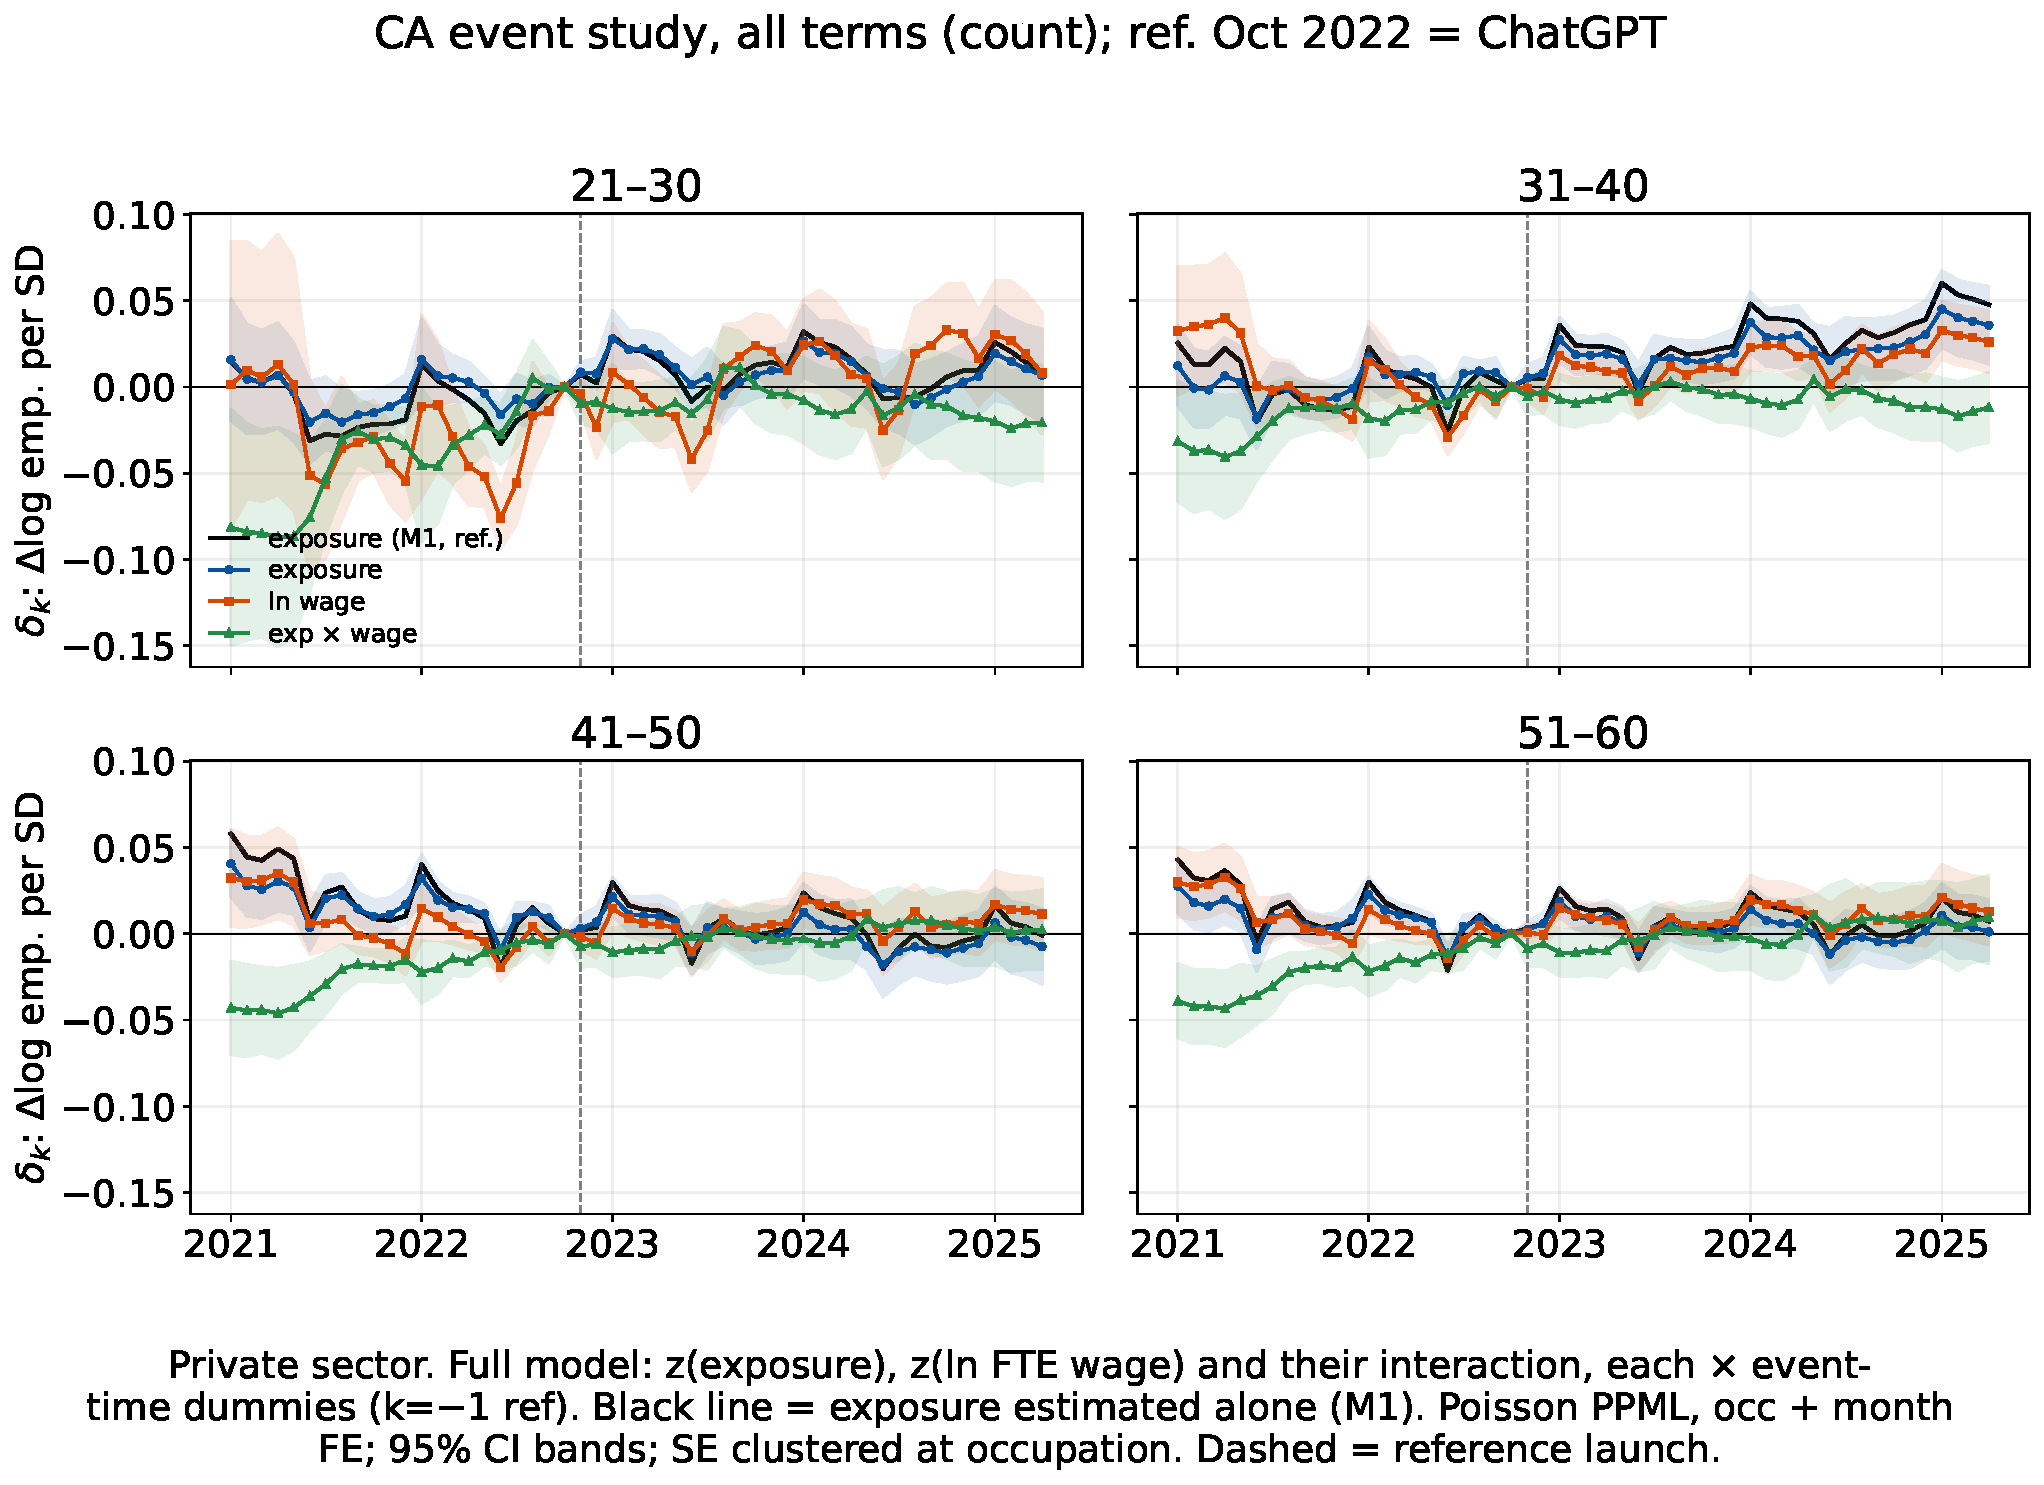
\includegraphics[width=\textwidth,height=0.42\textheight,keepaspectratio]{figure_ca_es_grid_stdexp.pdf}\\[4pt]
  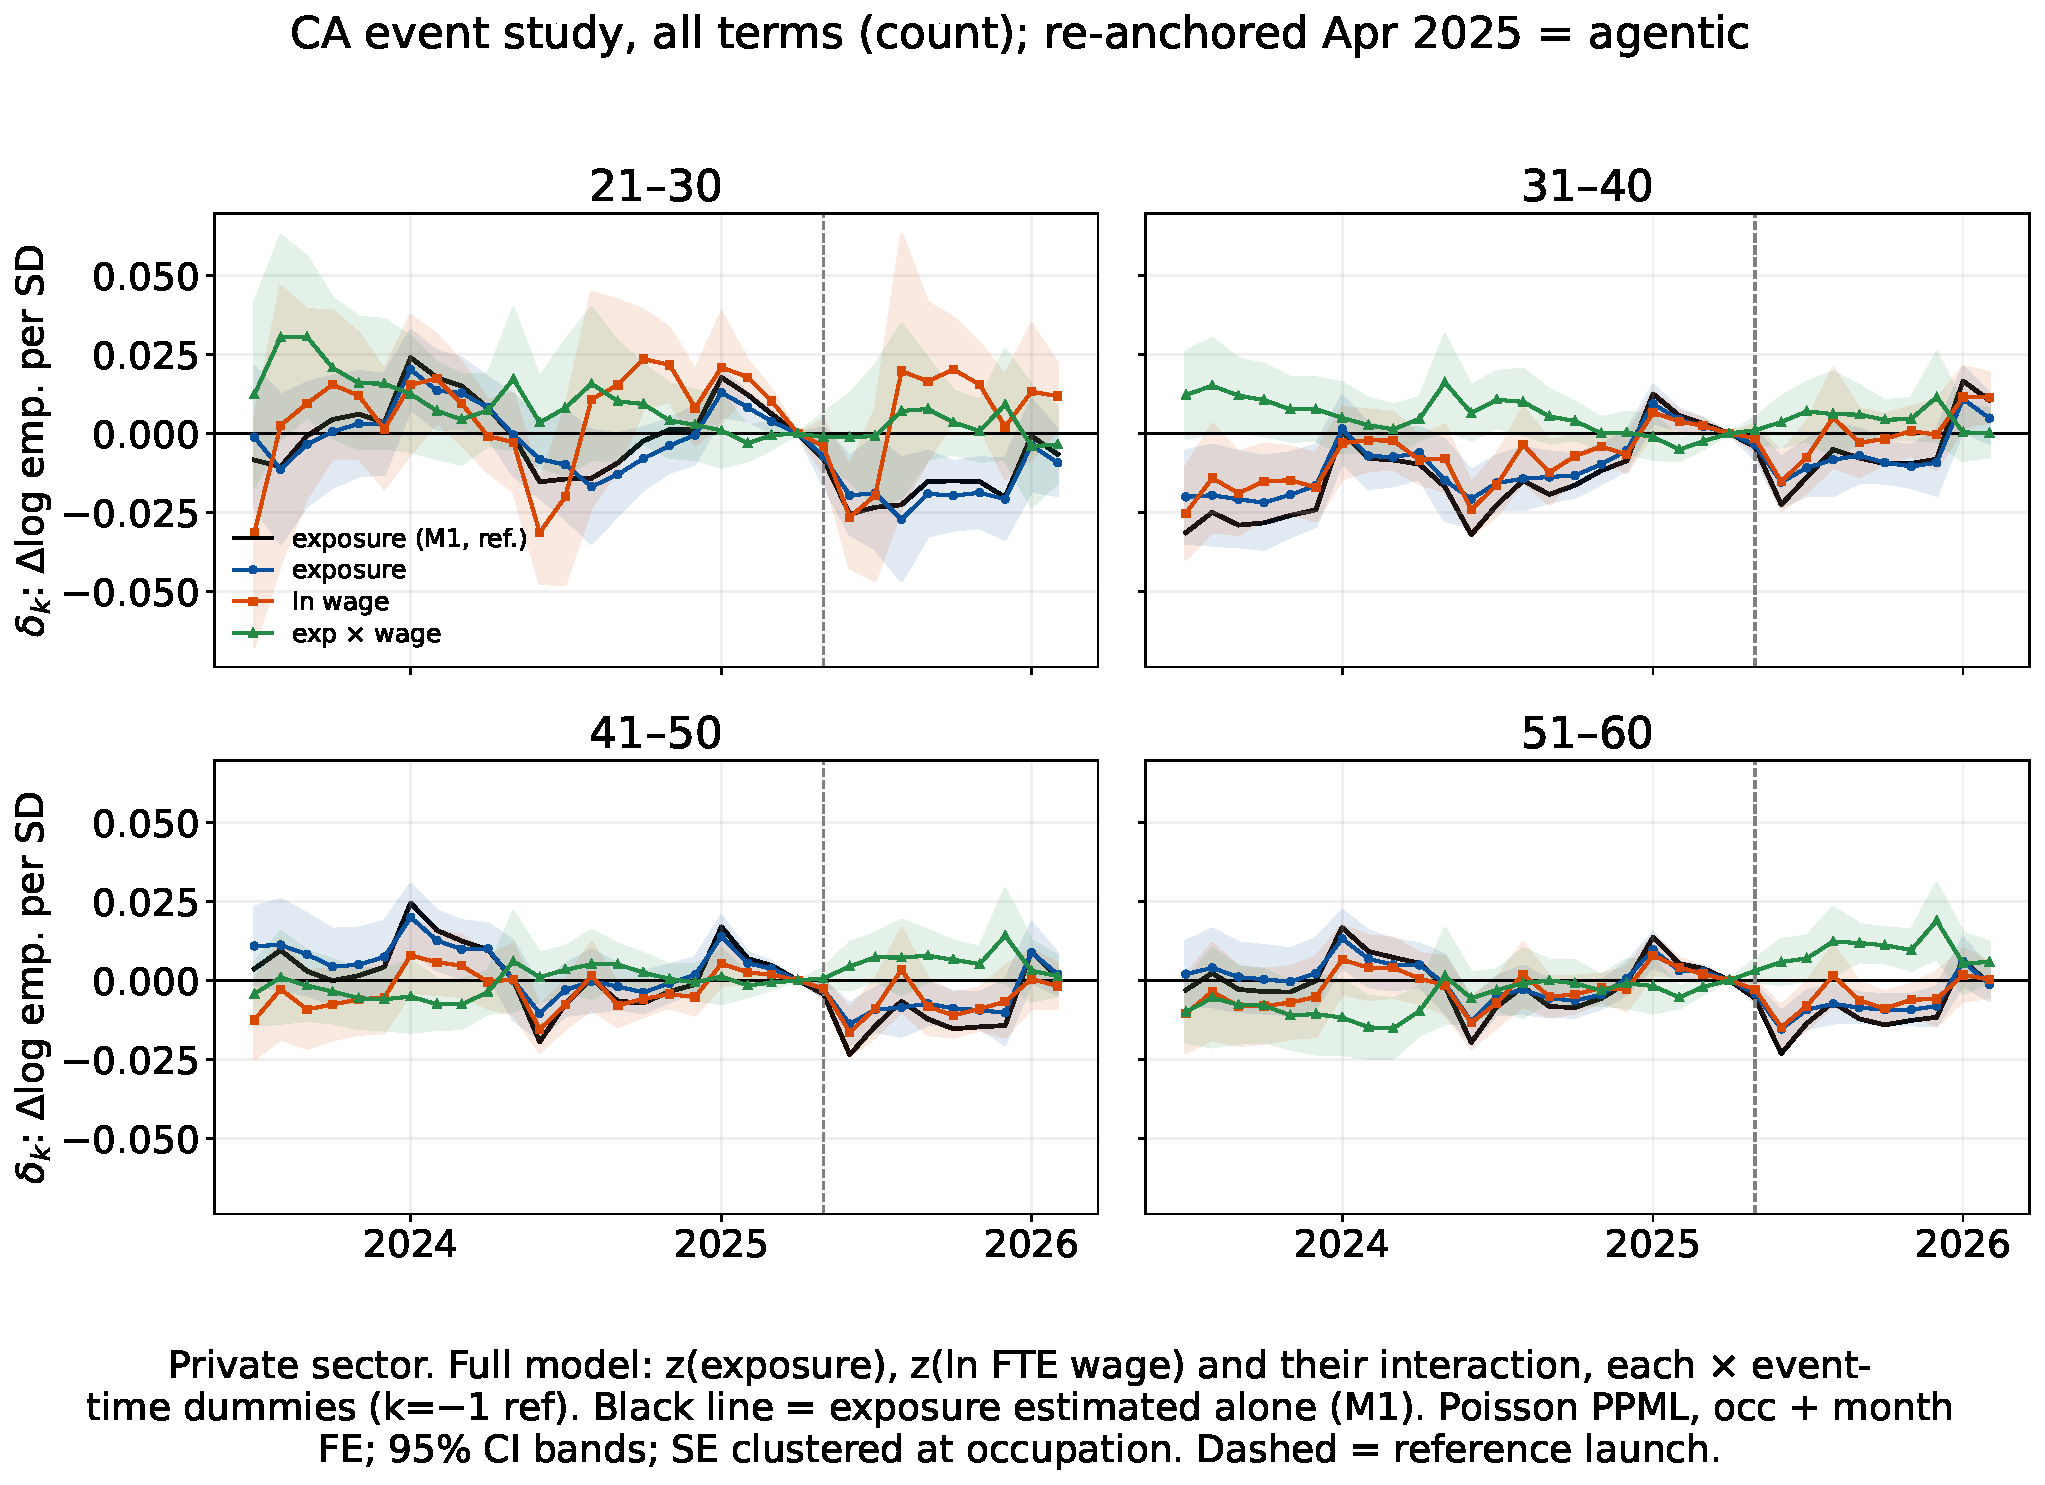
\includegraphics[width=\textwidth,height=0.42\textheight,keepaspectratio]{figure_ca_es_decade_agentic_stdexp.pdf}
  \caption{Employment (count): CA event study --- ChatGPT anchor (top),
           agentic anchor (bottom).}
\end{figure}

\clearpage
\subsection{New hires (nyjobb)}
\begin{figure}[H]\centering
  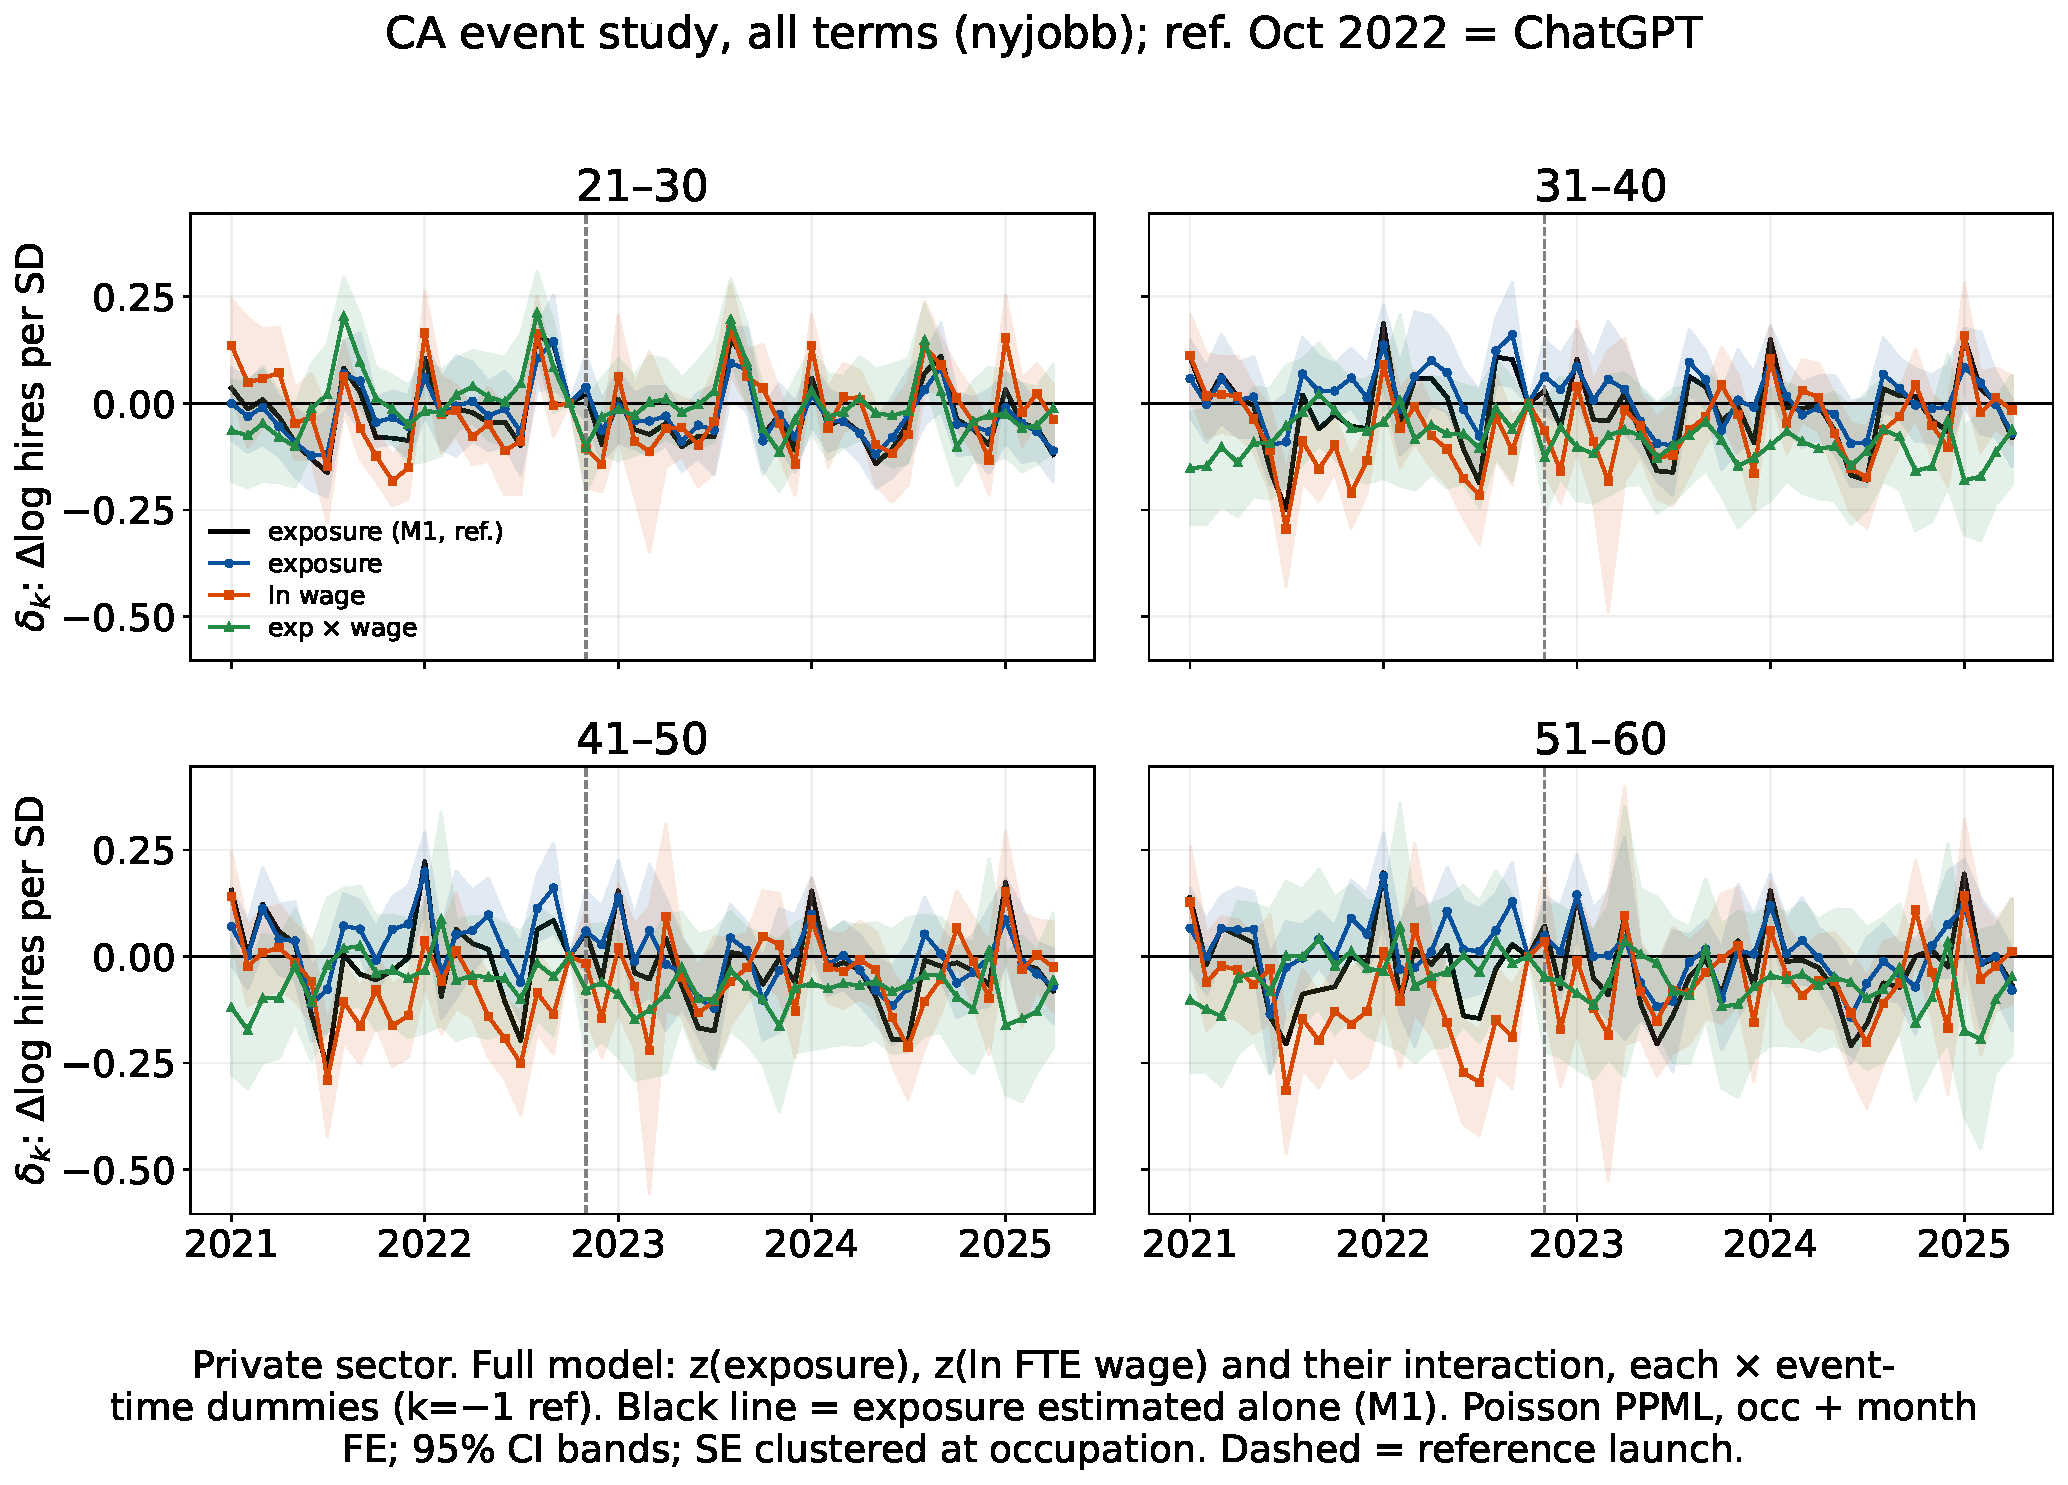
\includegraphics[width=\textwidth,height=0.42\textheight,keepaspectratio]{figure_ca_es_grid_stdexp_nyjobb.pdf}\\[4pt]
  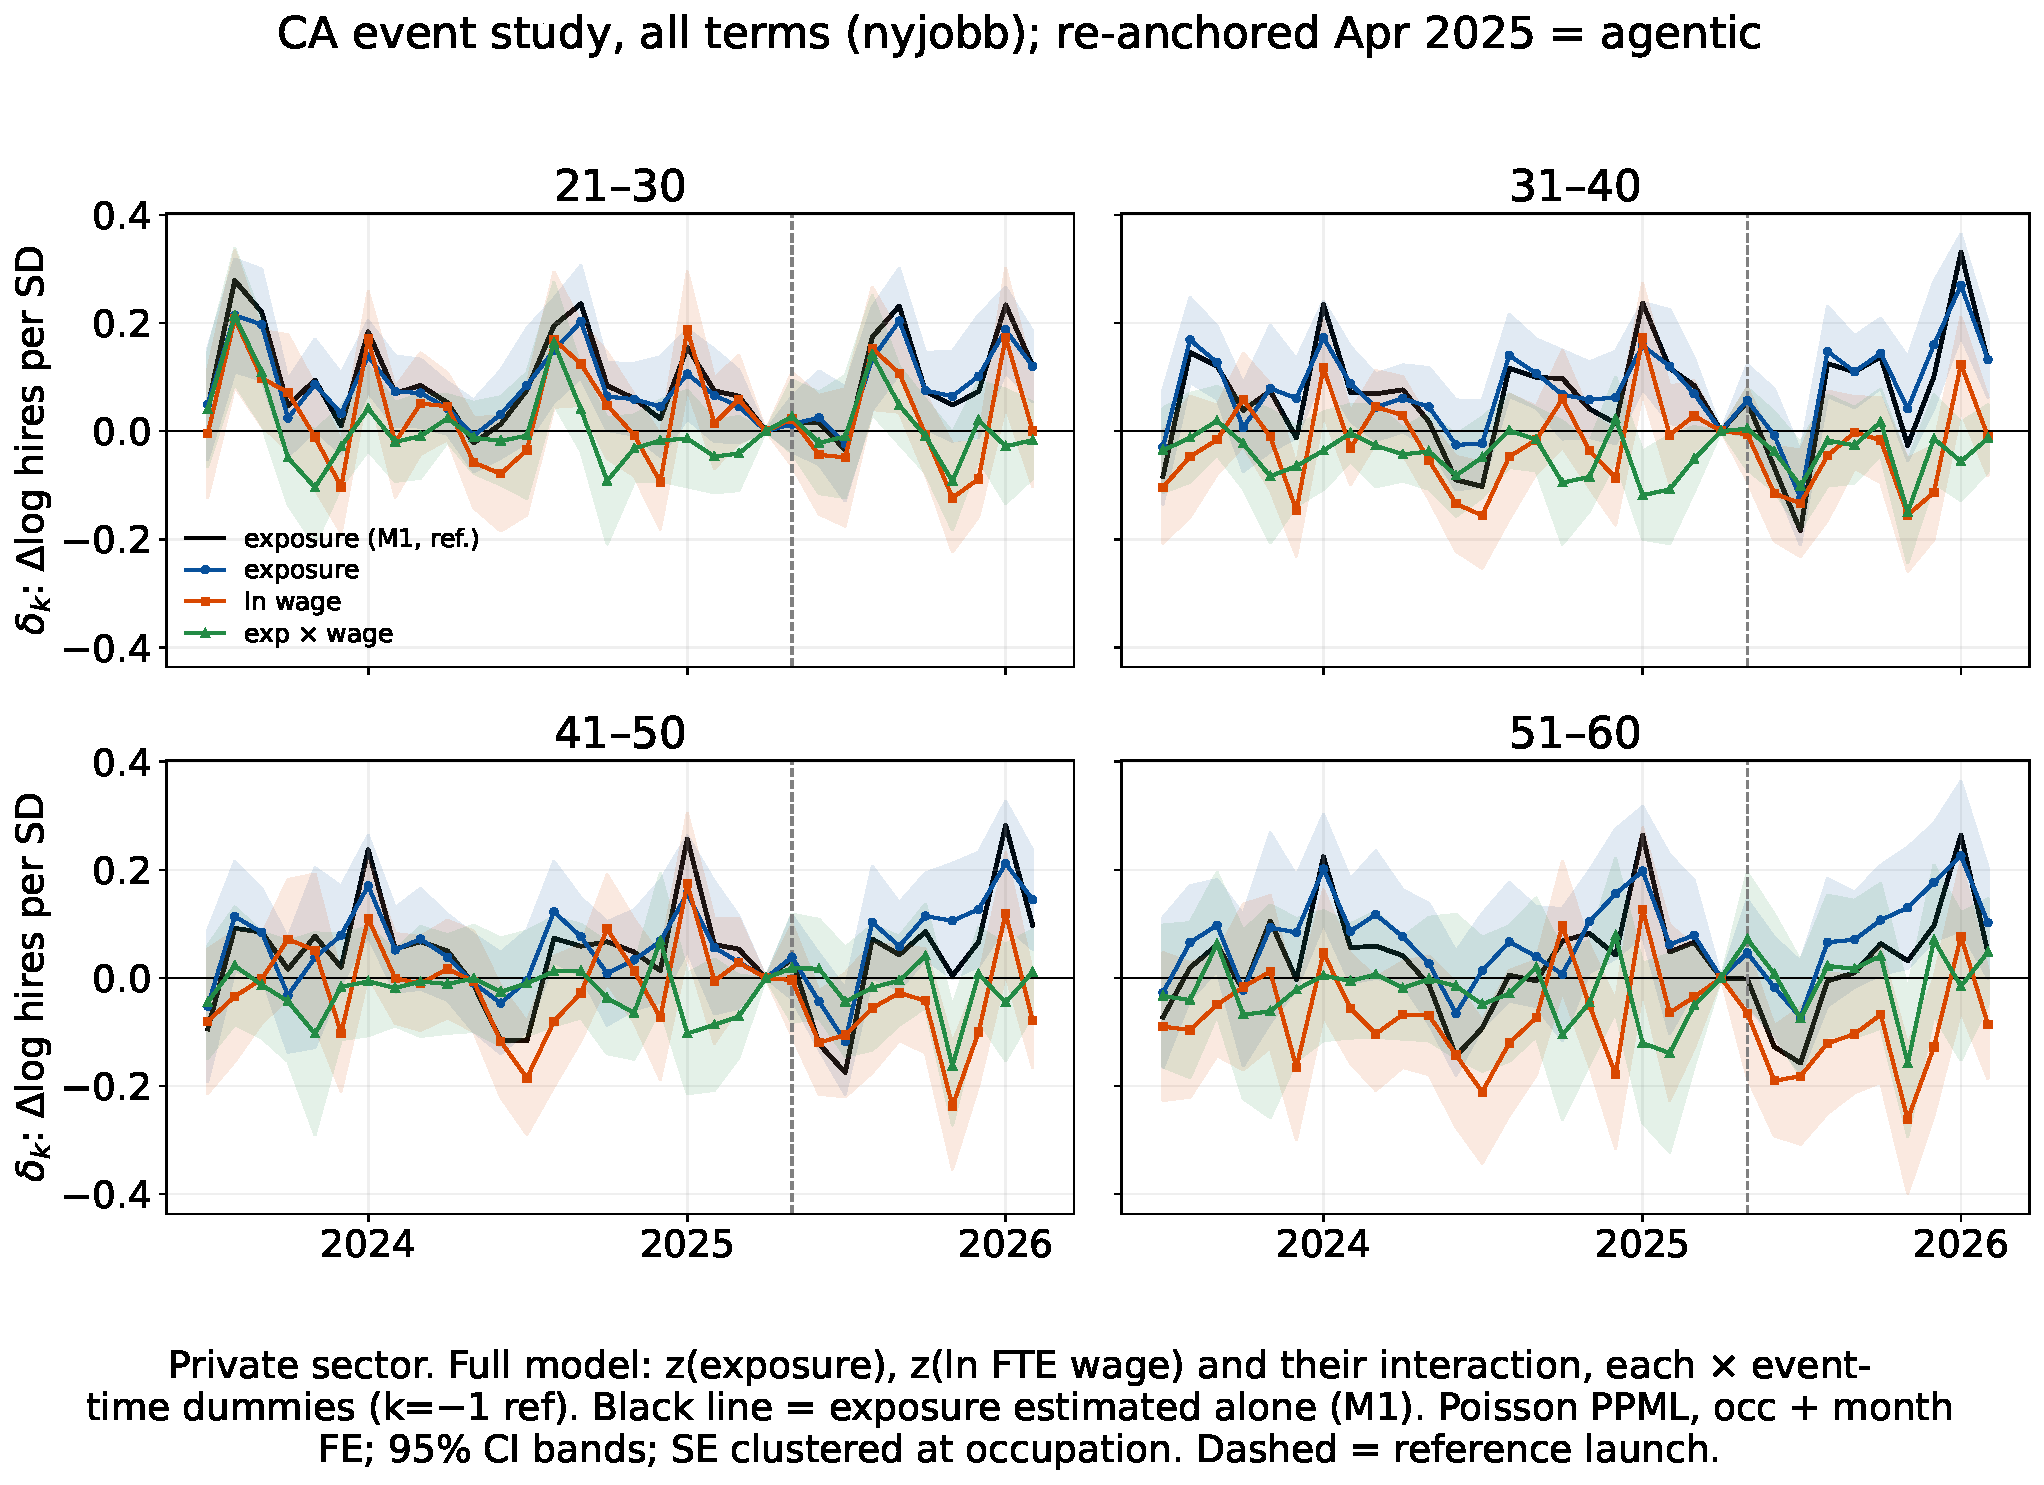
\includegraphics[width=\textwidth,height=0.42\textheight,keepaspectratio]{figure_ca_es_decade_agentic_stdexp_nyjobb.pdf}
  \caption{New hires (nyjobb): CA event study --- ChatGPT anchor (top),
           agentic anchor (bottom).}
\end{figure}

% =====================================================================
\clearpage
\section{Pooled post-treatment estimates (Poisson PPML DiD)}

\subsection{Employment (count)}
\begin{table}[H]\centering
\caption{AI exposure, wage, and private-sector employment headcount, by age group}
\label{tab:ca_did_combined}
\small
\begin{tabular}{lcccccc}
\toprule
 & \multicolumn{3}{c}{ChatGPT (ref.\ Oct 2022)} & \multicolumn{3}{c}{Agentic (ref.\ Apr 2025)} \\
\cmidrule(lr){2-4} \cmidrule(lr){5-7}
 & (1) & (2) & (3) & (4) & (5) & (6) \\
\midrule
\multicolumn{7}{@{}l}{\textit{Panel A: ages 21–30}} \\
Exposure $\times$ Post & +0.0104 &  & +0.0090 & -0.0154*** &  & -0.0165*** \\
 & (0.0070) &  & (0.0080) & (0.0053) &  & (0.0054) \\
ln wage $\times$ Post &  & +0.0116 & +0.0068 &  & -0.0004 & +0.0048 \\
 &  & (0.0085) & (0.0101) &  & (0.0084) & (0.0083) \\
Exp $\times$ wage $\times$ Post &  &  & -0.0104 &  &  & +0.0018 \\
 &  &  & (0.0106) &  &  & (0.0058) \\
\quad Observations & \multicolumn{3}{c}{20,176} & \multicolumn{3}{c}{12,320} \\
\quad Occupations & \multicolumn{3}{c}{388} & \multicolumn{3}{c}{385} \\
\midrule
\multicolumn{7}{@{}l}{\textit{Panel B: ages 31–40}} \\
Exposure $\times$ Post & +0.0291*** &  & +0.0225*** & -0.0054* &  & -0.0059* \\
 & (0.0061) &  & (0.0072) & (0.0031) &  & (0.0034) \\
ln wage $\times$ Post &  & +0.0256*** & +0.0142** &  & -0.0026 & -0.0001 \\
 &  & (0.0053) & (0.0056) &  & (0.0036) & (0.0039) \\
Exp $\times$ wage $\times$ Post &  &  & -0.0060 &  &  & +0.0046 \\
 &  &  & (0.0071) &  &  & (0.0035) \\
\quad Observations & \multicolumn{3}{c}{20,072} & \multicolumn{3}{c}{12,320} \\
\quad Occupations & \multicolumn{3}{c}{386} & \multicolumn{3}{c}{385} \\
\midrule
\multicolumn{7}{@{}l}{\textit{Panel C: ages 41–50}} \\
Exposure $\times$ Post & +0.0041 &  & +0.0000 & -0.0096*** &  & -0.0060** \\
 & (0.0060) &  & (0.0072) & (0.0023) &  & (0.0026) \\
ln wage $\times$ Post &  & +0.0070 & +0.0070 &  & -0.0090*** & -0.0061* \\
 &  & (0.0057) & (0.0067) &  & (0.0029) & (0.0033) \\
Exp $\times$ wage $\times$ Post &  &  & -0.0008 &  &  & +0.0058* \\
 &  &  & (0.0086) &  &  & (0.0030) \\
\quad Observations & \multicolumn{3}{c}{20,124} & \multicolumn{3}{c}{12,320} \\
\quad Occupations & \multicolumn{3}{c}{387} & \multicolumn{3}{c}{385} \\
\midrule
\multicolumn{7}{@{}l}{\textit{Panel D: ages 51–60}} \\
Exposure $\times$ Post & +0.0076 &  & +0.0030 & -0.0095*** &  & -0.0067*** \\
 & (0.0054) &  & (0.0060) & (0.0019) &  & (0.0019) \\
ln wage $\times$ Post &  & +0.0108** & +0.0092 &  & -0.0074*** & -0.0050** \\
 &  & (0.0053) & (0.0060) &  & (0.0021) & (0.0022) \\
Exp $\times$ wage $\times$ Post &  &  & +0.0005 &  &  & +0.0091*** \\
 &  &  & (0.0088) &  &  & (0.0023) \\
\quad Observations & \multicolumn{3}{c}{20,176} & \multicolumn{3}{c}{12,352} \\
\quad Occupations & \multicolumn{3}{c}{388} & \multicolumn{3}{c}{386} \\
\midrule
Occupation FE & Yes & Yes & Yes & Yes & Yes & Yes \\
Month FE & Yes & Yes & Yes & Yes & Yes & Yes \\
\bottomrule
\end{tabular}
\begin{minipage}{\linewidth}\vspace{2pt}\footnotesize
\emph{Notes:} Poisson PPML (cell-level employment headcount, private sector). Columns (1)--(3): ChatGPT window (Oct 2022 $=k{=}{-}1$, through 2025m4); (4)--(6): agentic (Apr 2025 $=k{=}{-}1$, from 2023m7). Each coefficient is the average post-period effect relative to the reference month ($k{=}{-}1$); each pre-period month enters as a separate control. M1 = exposure only, M2 = ln wage only, M3 = both $+$ interaction. Treatments standardized: $z(\text{exp})$ = Eloundou $\beta$ (pooled), $z(\text{lnw})$ = ln full-time-equivalent wage within age group. Occupation and month fixed effects in all columns; SE clustered at occupation in parentheses; coefficients are $\Delta\log$ per 1 SD. Pseudo $R^2 \approx 0.99$ (FE-driven). $^{*}p<0.10$, $^{**}p<0.05$, $^{***}p<0.01$.
\end{minipage}
\end{table}

\clearpage
\subsection{New hires (nyjobb)}
\begin{table}[H]\centering
\caption{AI exposure, wage, and private-sector new hires = round(count $\times$ ny\_jobb), by age group}
\label{tab:ca_did_combined_nyjobb}
\small
\begin{tabular}{lcccccc}
\toprule
 & \multicolumn{3}{c}{ChatGPT (ref.\ Oct 2022)} & \multicolumn{3}{c}{Agentic (ref.\ Apr 2025)} \\
\cmidrule(lr){2-4} \cmidrule(lr){5-7}
 & (1) & (2) & (3) & (4) & (5) & (6) \\
\midrule
\multicolumn{7}{@{}l}{\textit{Panel A: ages 21–30}} \\
Exposure $\times$ Post & -0.0264 &  & -0.0240 & +0.1014*** &  & +0.0971*** \\
 & (0.0264) &  & (0.0282) & (0.0266) &  & (0.0289) \\
ln wage $\times$ Post &  & -0.0166 & -0.0089 &  & +0.0494 & +0.0230 \\
 &  & (0.0233) & (0.0261) &  & (0.0329) & (0.0327) \\
Exp $\times$ wage $\times$ Post &  &  & -0.0007 &  &  & +0.0151 \\
 &  &  & (0.0371) &  &  & (0.0257) \\
\quad Observations & \multicolumn{3}{c}{19,136} & \multicolumn{3}{c}{11,744} \\
\quad Occupations & \multicolumn{3}{c}{368} & \multicolumn{3}{c}{367} \\
\midrule
\multicolumn{7}{@{}l}{\textit{Panel B: ages 31–40}} \\
Exposure $\times$ Post & -0.0074 &  & +0.0121 & +0.0885*** &  & +0.1071*** \\
 & (0.0359) &  & (0.0323) & (0.0232) &  & (0.0269) \\
ln wage $\times$ Post &  & -0.0293 & -0.0352 &  & +0.0186 & -0.0368 \\
 &  & (0.0362) & (0.0329) &  & (0.0265) & (0.0278) \\
Exp $\times$ wage $\times$ Post &  &  & -0.0978* &  &  & -0.0284 \\
 &  &  & (0.0562) &  &  & (0.0229) \\
\quad Observations & \multicolumn{3}{c}{19,188} & \multicolumn{3}{c}{11,648} \\
\quad Occupations & \multicolumn{3}{c}{369} & \multicolumn{3}{c}{364} \\
\midrule
\multicolumn{7}{@{}l}{\textit{Panel C: ages 41–50}} \\
Exposure $\times$ Post & -0.0126 &  & -0.0013 & +0.0558*** &  & +0.0874** \\
 & (0.0365) &  & (0.0280) & (0.0214) &  & (0.0343) \\
ln wage $\times$ Post &  & -0.0295 & -0.0292 &  & -0.0074 & -0.0553 \\
 &  & (0.0392) & (0.0386) &  & (0.0294) & (0.0385) \\
Exp $\times$ wage $\times$ Post &  &  & -0.0802 &  &  & -0.0117 \\
 &  &  & (0.0661) &  &  & (0.0339) \\
\quad Observations & \multicolumn{3}{c}{18,980} & \multicolumn{3}{c}{11,616} \\
\quad Occupations & \multicolumn{3}{c}{365} & \multicolumn{3}{c}{363} \\
\midrule
\multicolumn{7}{@{}l}{\textit{Panel D: ages 51–60}} \\
Exposure $\times$ Post & -0.0069 &  & +0.0077 & +0.0438 &  & +0.1011** \\
 & (0.0371) &  & (0.0290) & (0.0284) &  & (0.0411) \\
ln wage $\times$ Post &  & -0.0373 & -0.0395 &  & -0.0490 & -0.1005** \\
 &  & (0.0467) & (0.0509) &  & (0.0402) & (0.0481) \\
Exp $\times$ wage $\times$ Post &  &  & -0.0653 &  &  & +0.0094 \\
 &  &  & (0.0742) &  &  & (0.0485) \\
\quad Observations & \multicolumn{3}{c}{18,980} & \multicolumn{3}{c}{11,392} \\
\quad Occupations & \multicolumn{3}{c}{365} & \multicolumn{3}{c}{356} \\
\midrule
Occupation FE & Yes & Yes & Yes & Yes & Yes & Yes \\
Month FE & Yes & Yes & Yes & Yes & Yes & Yes \\
\bottomrule
\end{tabular}
\begin{minipage}{\linewidth}\vspace{2pt}\footnotesize
\emph{Notes:} Poisson PPML (cell-level new hires = round(count $\times$ ny\_jobb), private sector). Columns (1)--(3): ChatGPT window (Oct 2022 $=k{=}{-}1$, through 2025m4); (4)--(6): agentic (Apr 2025 $=k{=}{-}1$, from 2023m7). Each coefficient is the average post-period effect relative to the reference month ($k{=}{-}1$); each pre-period month enters as a separate control. M1 = exposure only, M2 = ln wage only, M3 = both $+$ interaction. Treatments standardized: $z(\text{exp})$ = Eloundou $\beta$ (pooled), $z(\text{lnw})$ = ln full-time-equivalent wage within age group. Occupation and month fixed effects in all columns; SE clustered at occupation in parentheses; coefficients are $\Delta\log$ per 1 SD. Pseudo $R^2 \approx 0.99$ (FE-driven). $^{*}p<0.10$, $^{**}p<0.05$, $^{***}p<0.01$.
\end{minipage}
\end{table}

% =====================================================================
\clearpage
\section{Log-employment OLS (alternative estimator)}

\noindent
Sections 1--2 use Poisson PPML on counts (robust to zero cells; implicitly
employment-weighted). This section uses an alternative estimator: \emph{OLS on
log employment}, with occupation and month fixed effects. To keep it
employment-representative --- comparable to PPML --- each cell is weighted by the
occupation $\times$ age group's \emph{baseline} (pre-period) employment, and
zero-employment cells are dropped (logs).

\subsection{Event study}
\begin{figure}[H]\centering
  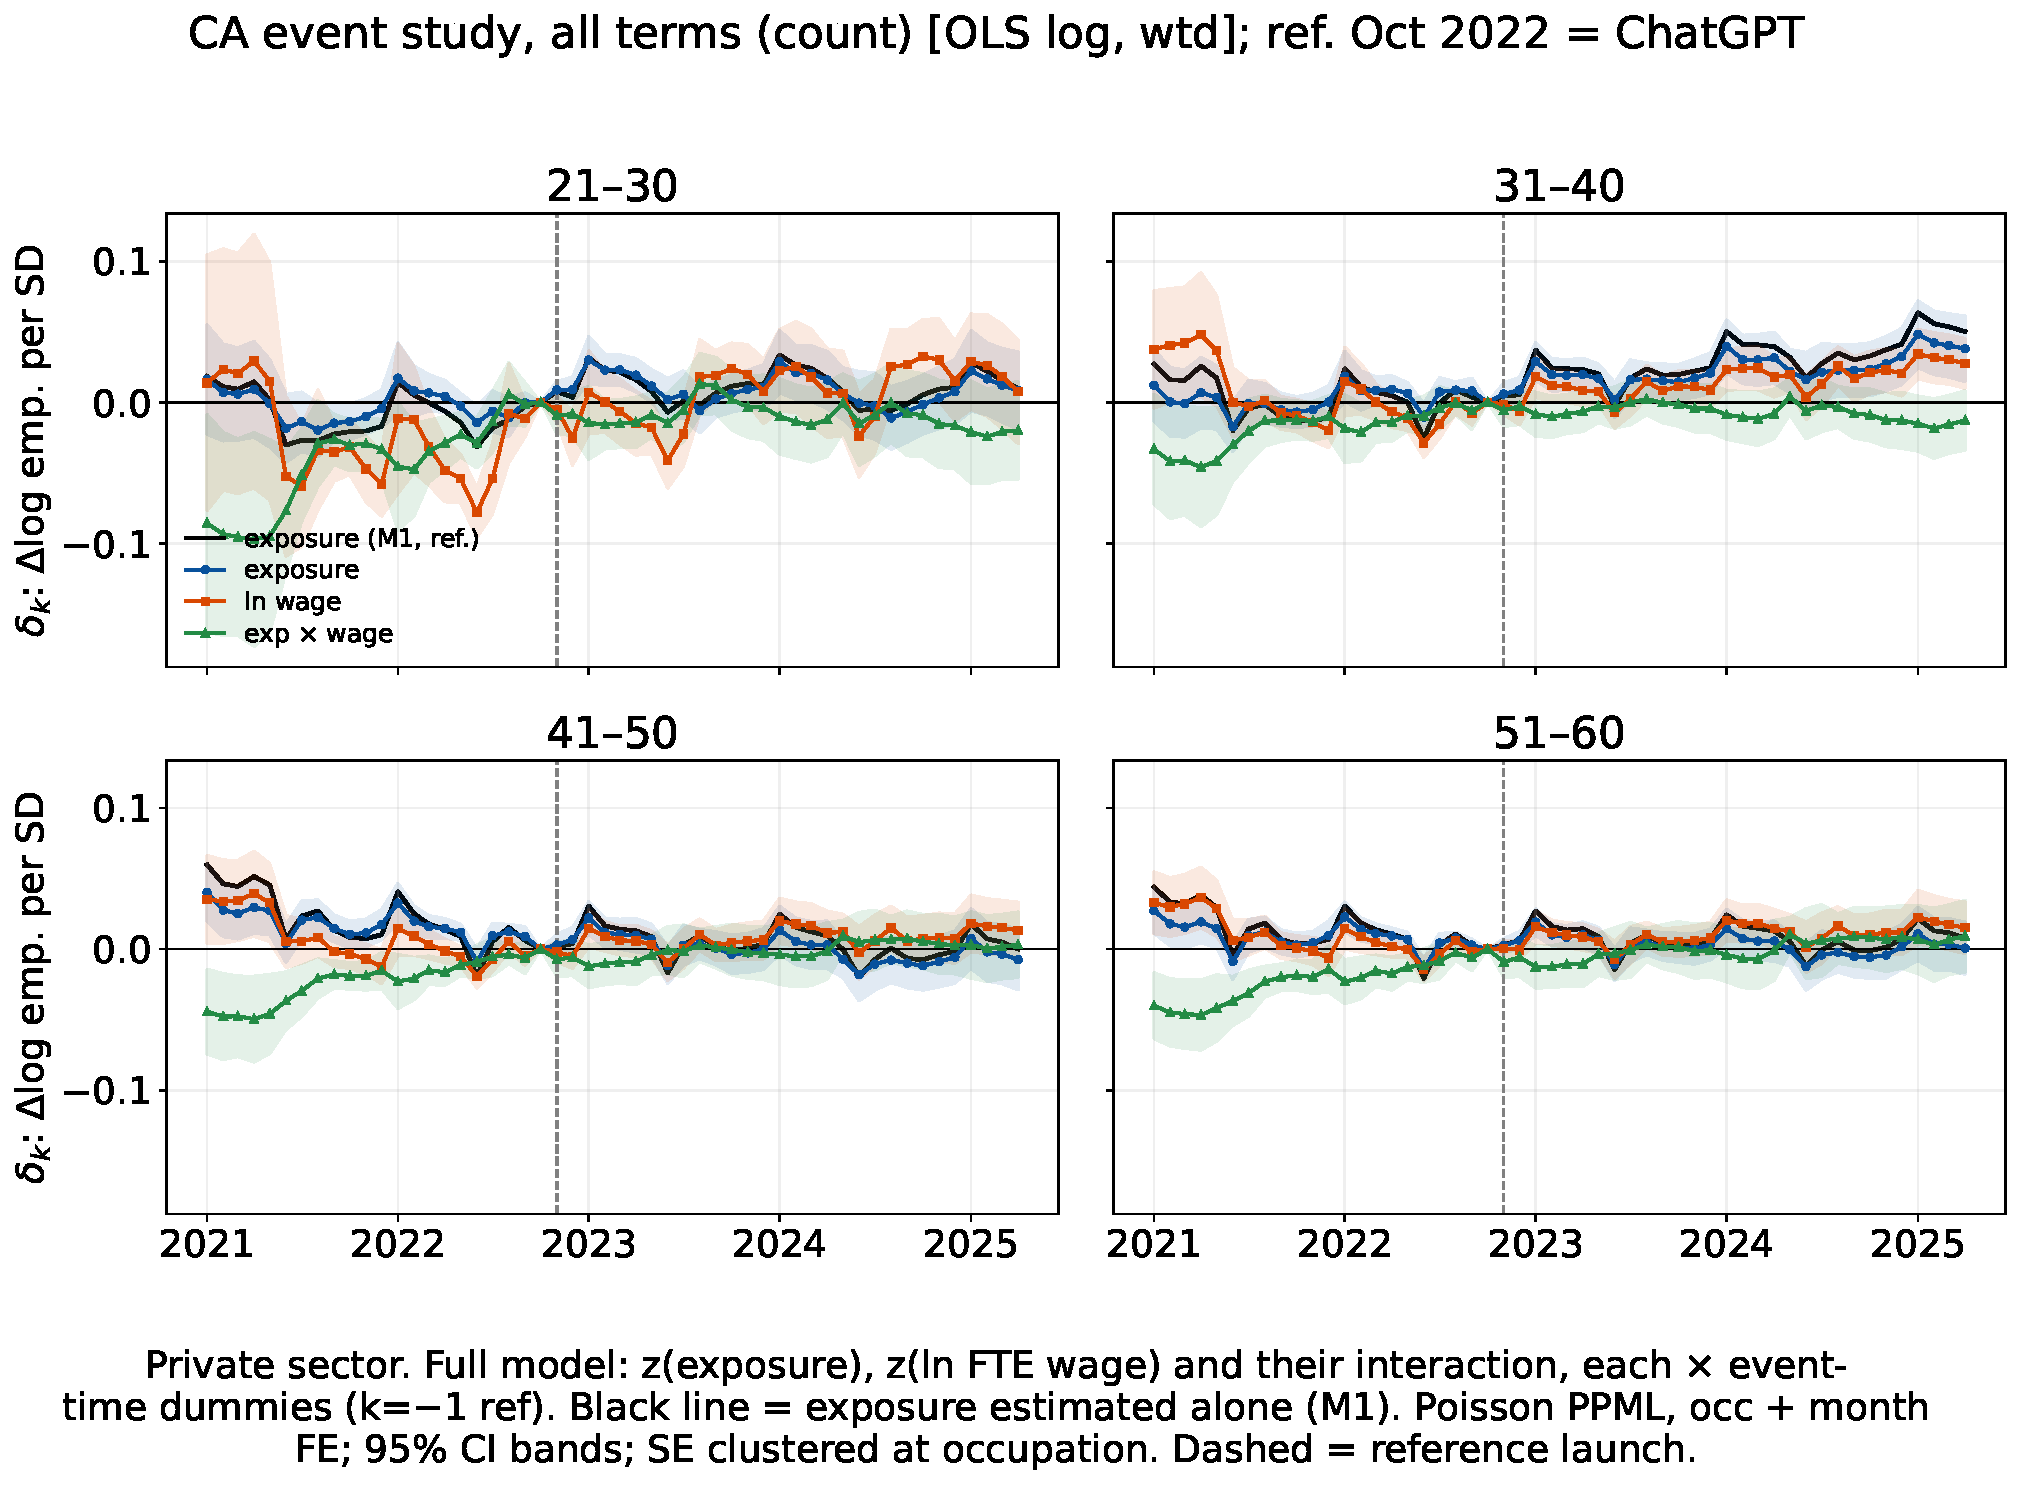
\includegraphics[width=\textwidth,height=0.42\textheight,keepaspectratio]{figure_ca_es_grid_stdexp_olslog.pdf}\\[4pt]
  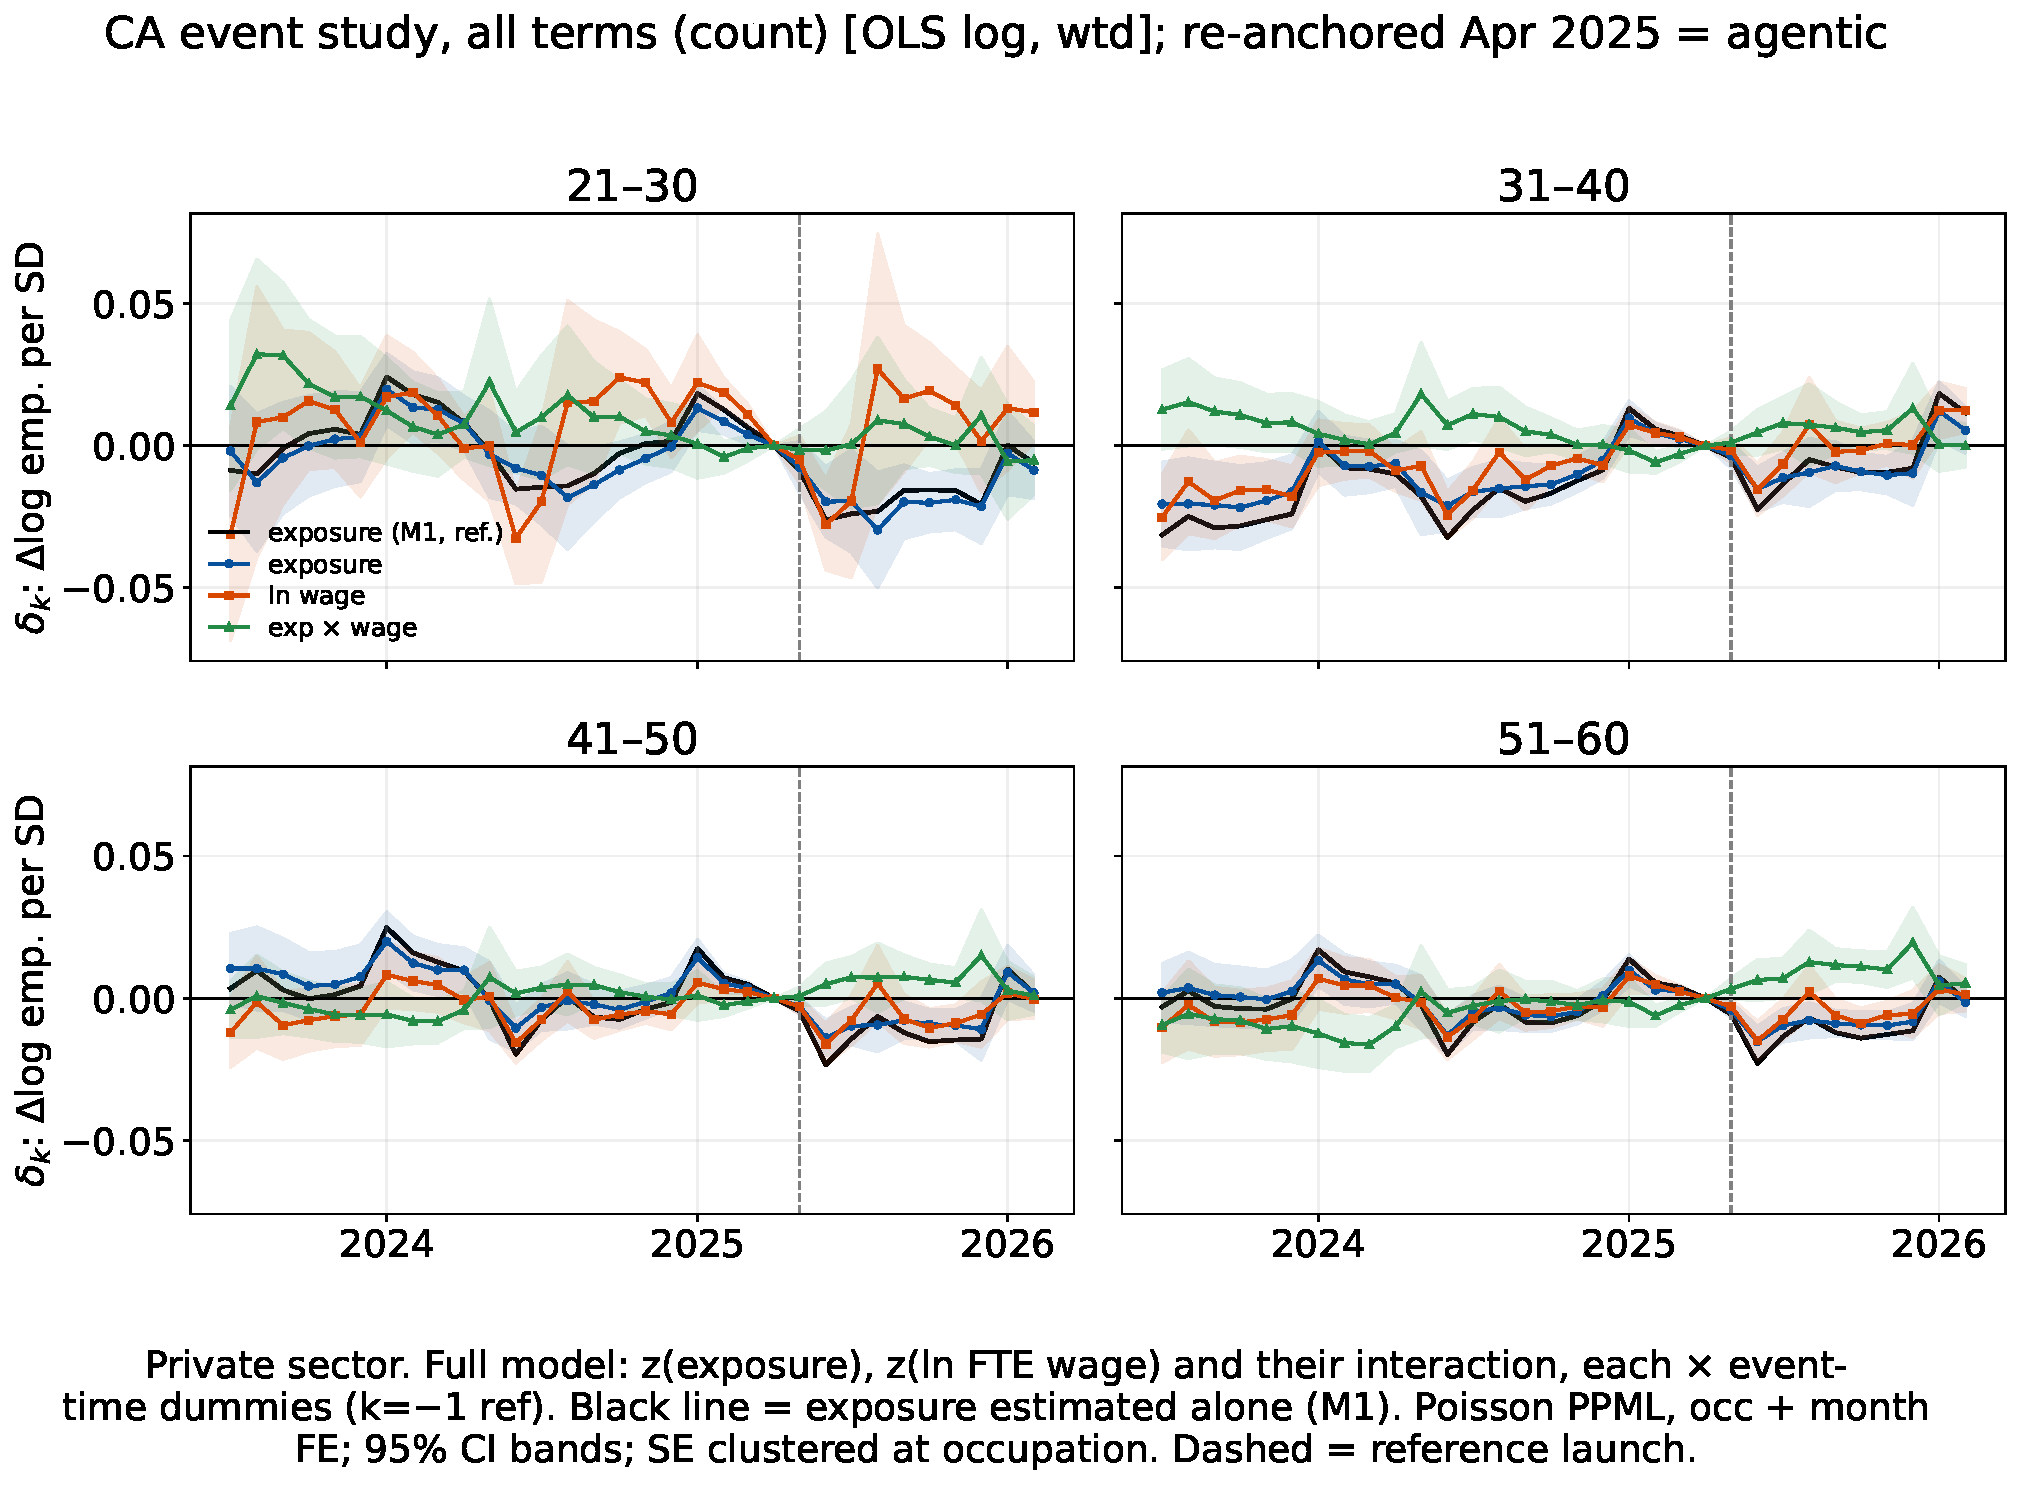
\includegraphics[width=\textwidth,height=0.42\textheight,keepaspectratio]{figure_ca_es_decade_agentic_stdexp_olslog.pdf}
  \caption{Log employment (OLS, baseline-weighted): CA event study ---
           ChatGPT anchor (top), agentic anchor (bottom).}
\end{figure}

\clearpage
\subsection{Pooled post-treatment (DiD)}
\begin{table}[H]\centering
\caption{AI exposure, wage, and private-sector log employment, by age group}
\label{tab:ca_did_combined_olslog}
\small
\begin{tabular}{lcccccc}
\toprule
 & \multicolumn{3}{c}{ChatGPT (ref.\ Oct 2022)} & \multicolumn{3}{c}{Agentic (ref.\ Apr 2025)} \\
\cmidrule(lr){2-4} \cmidrule(lr){5-7}
 & (1) & (2) & (3) & (4) & (5) & (6) \\
\midrule
\multicolumn{7}{@{}l}{\textit{Panel A: ages 21–30}} \\
Exposure $\times$ Post & +0.0113 &  & +0.0098 & -0.0156*** &  & -0.0168*** \\
 & (0.0072) &  & (0.0081) & (0.0052) &  & (0.0053) \\
ln wage $\times$ Post &  & +0.0120 & +0.0073 &  & -0.0005 & +0.0051 \\
 &  & (0.0094) & (0.0108) &  & (0.0086) & (0.0086) \\
Exp $\times$ wage $\times$ Post &  &  & -0.0100 &  &  & +0.0017 \\
 &  &  & (0.0109) &  &  & (0.0060) \\
\quad Observations & \multicolumn{3}{c}{19,332} & \multicolumn{3}{c}{11,955} \\
\quad Occupations & \multicolumn{3}{c}{390} & \multicolumn{3}{c}{387} \\
\midrule
\multicolumn{7}{@{}l}{\textit{Panel B: ages 31–40}} \\
Exposure $\times$ Post & +0.0303*** &  & +0.0236*** & -0.0050* &  & -0.0059* \\
 & (0.0062) &  & (0.0074) & (0.0030) &  & (0.0034) \\
ln wage $\times$ Post &  & +0.0270*** & +0.0151*** &  & -0.0020 & +0.0006 \\
 &  & (0.0055) & (0.0057) &  & (0.0035) & (0.0040) \\
Exp $\times$ wage $\times$ Post &  &  & -0.0070 &  &  & +0.0051 \\
 &  &  & (0.0075) &  &  & (0.0036) \\
\quad Observations & \multicolumn{3}{c}{19,427} & \multicolumn{3}{c}{11,962} \\
\quad Occupations & \multicolumn{3}{c}{387} & \multicolumn{3}{c}{386} \\
\midrule
\multicolumn{7}{@{}l}{\textit{Panel C: ages 41–50}} \\
Exposure $\times$ Post & +0.0045 &  & -0.0000 & -0.0093*** &  & -0.0062** \\
 & (0.0062) &  & (0.0072) & (0.0022) &  & (0.0026) \\
ln wage $\times$ Post &  & +0.0080 & +0.0080 &  & -0.0080*** & -0.0052 \\
 &  & (0.0058) & (0.0066) &  & (0.0027) & (0.0032) \\
Exp $\times$ wage $\times$ Post &  &  & -0.0007 &  &  & +0.0059** \\
 &  &  & (0.0087) &  &  & (0.0029) \\
\quad Observations & \multicolumn{3}{c}{19,360} & \multicolumn{3}{c}{11,896} \\
\quad Occupations & \multicolumn{3}{c}{387} & \multicolumn{3}{c}{382} \\
\midrule
\multicolumn{7}{@{}l}{\textit{Panel D: ages 51–60}} \\
Exposure $\times$ Post & +0.0078 &  & +0.0028 & -0.0092*** &  & -0.0068*** \\
 & (0.0055) &  & (0.0060) & (0.0019) &  & (0.0019) \\
ln wage $\times$ Post &  & +0.0118** & +0.0103* &  & -0.0068*** & -0.0045** \\
 &  & (0.0053) & (0.0059) &  & (0.0021) & (0.0022) \\
Exp $\times$ wage $\times$ Post &  &  & +0.0001 &  &  & +0.0092*** \\
 &  &  & (0.0091) &  &  & (0.0023) \\
\quad Observations & \multicolumn{3}{c}{19,309} & \multicolumn{3}{c}{11,908} \\
\quad Occupations & \multicolumn{3}{c}{389} & \multicolumn{3}{c}{386} \\
\midrule
Occupation FE & Yes & Yes & Yes & Yes & Yes & Yes \\
Month FE & Yes & Yes & Yes & Yes & Yes & Yes \\
\bottomrule
\end{tabular}
\begin{minipage}{\linewidth}\vspace{2pt}\footnotesize
\emph{Notes:} OLS on log employment, weighted by baseline (pre-period) employment (zero cells dropped) (cell-level log employment, private sector). Columns (1)--(3): ChatGPT window (Oct 2022 $=k{=}{-}1$, through 2025m4); (4)--(6): agentic (Apr 2025 $=k{=}{-}1$, from 2023m7). Each coefficient is the average post-period effect relative to the reference month ($k{=}{-}1$); each pre-period month enters as a separate control. M1 = exposure only, M2 = ln wage only, M3 = both $+$ interaction. Treatments standardized: $z(\text{exp})$ = Eloundou $\beta$ (pooled), $z(\text{lnw})$ = ln full-time-equivalent wage within age group. Occupation and month fixed effects in all columns; SE clustered at occupation in parentheses; coefficients are $\Delta\log$ per 1 SD. $^{*}p<0.10$, $^{**}p<0.05$, $^{***}p<0.01$.
\end{minipage}
\end{table}

% =====================================================================
\clearpage
\section{Log new-hires OLS (alternative estimator)}

\noindent
The same OLS-on-logs estimator applied to new hires. Because hires are a small
flow, taking logs drops cell-months with zero hires (a selected subsample);
PPML in Section~2 handles these directly and is preferred for hires. Weighted by
baseline (pre-period) hires.

\subsection{Event study}
\begin{figure}[H]\centering
  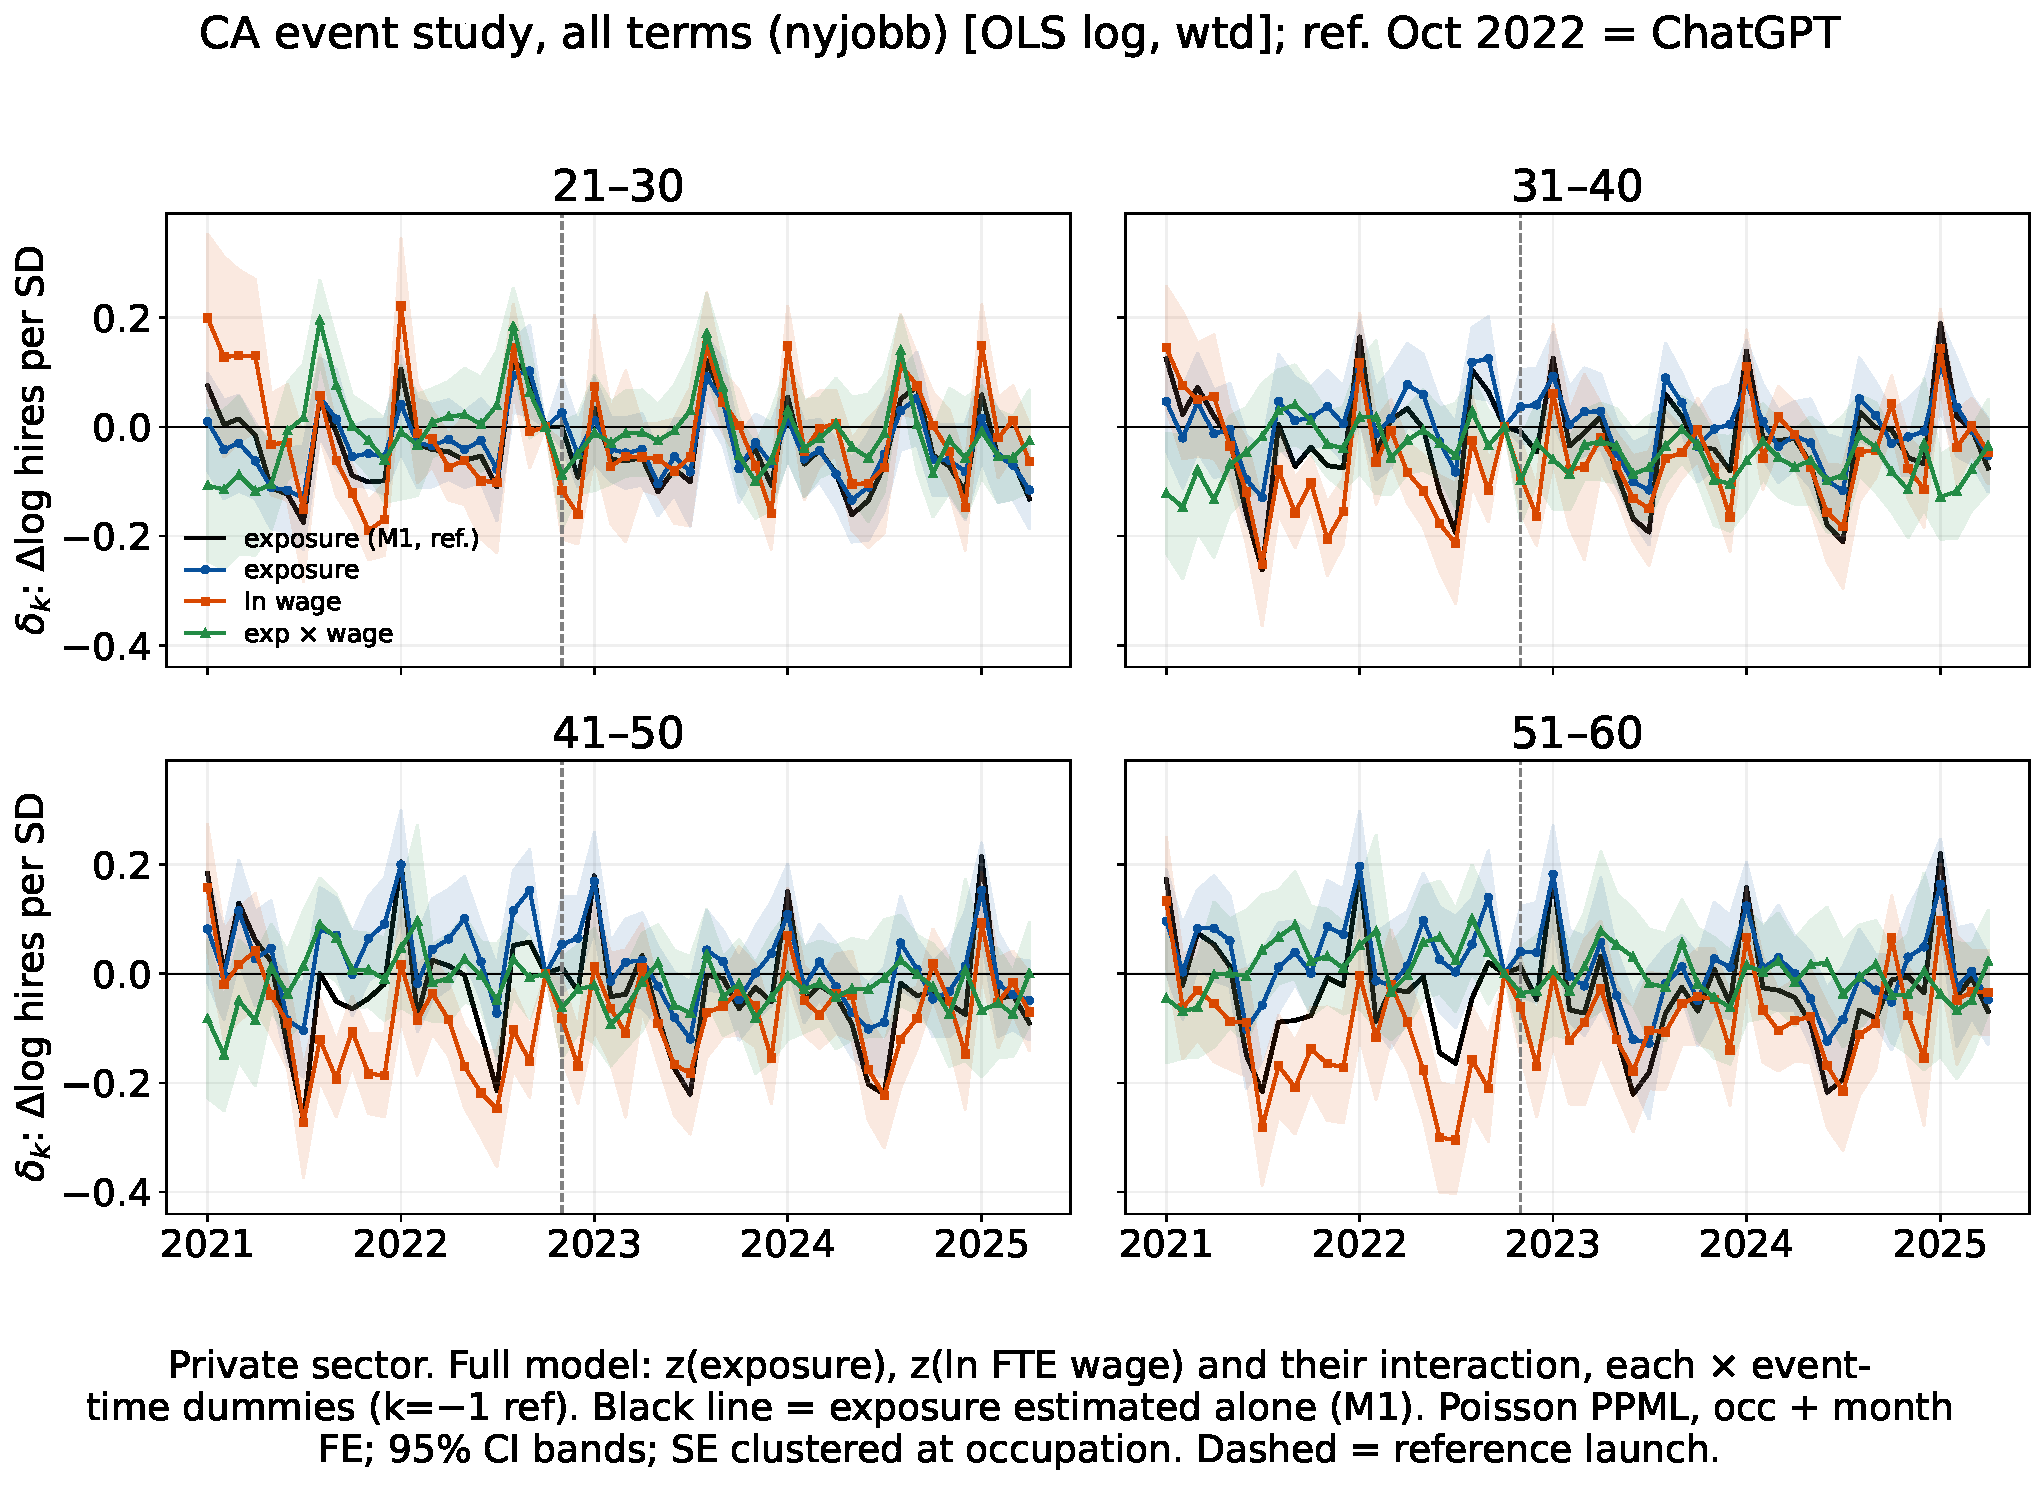
\includegraphics[width=\textwidth,height=0.42\textheight,keepaspectratio]{figure_ca_es_grid_stdexp_nyjobb_olslog.pdf}\\[4pt]
  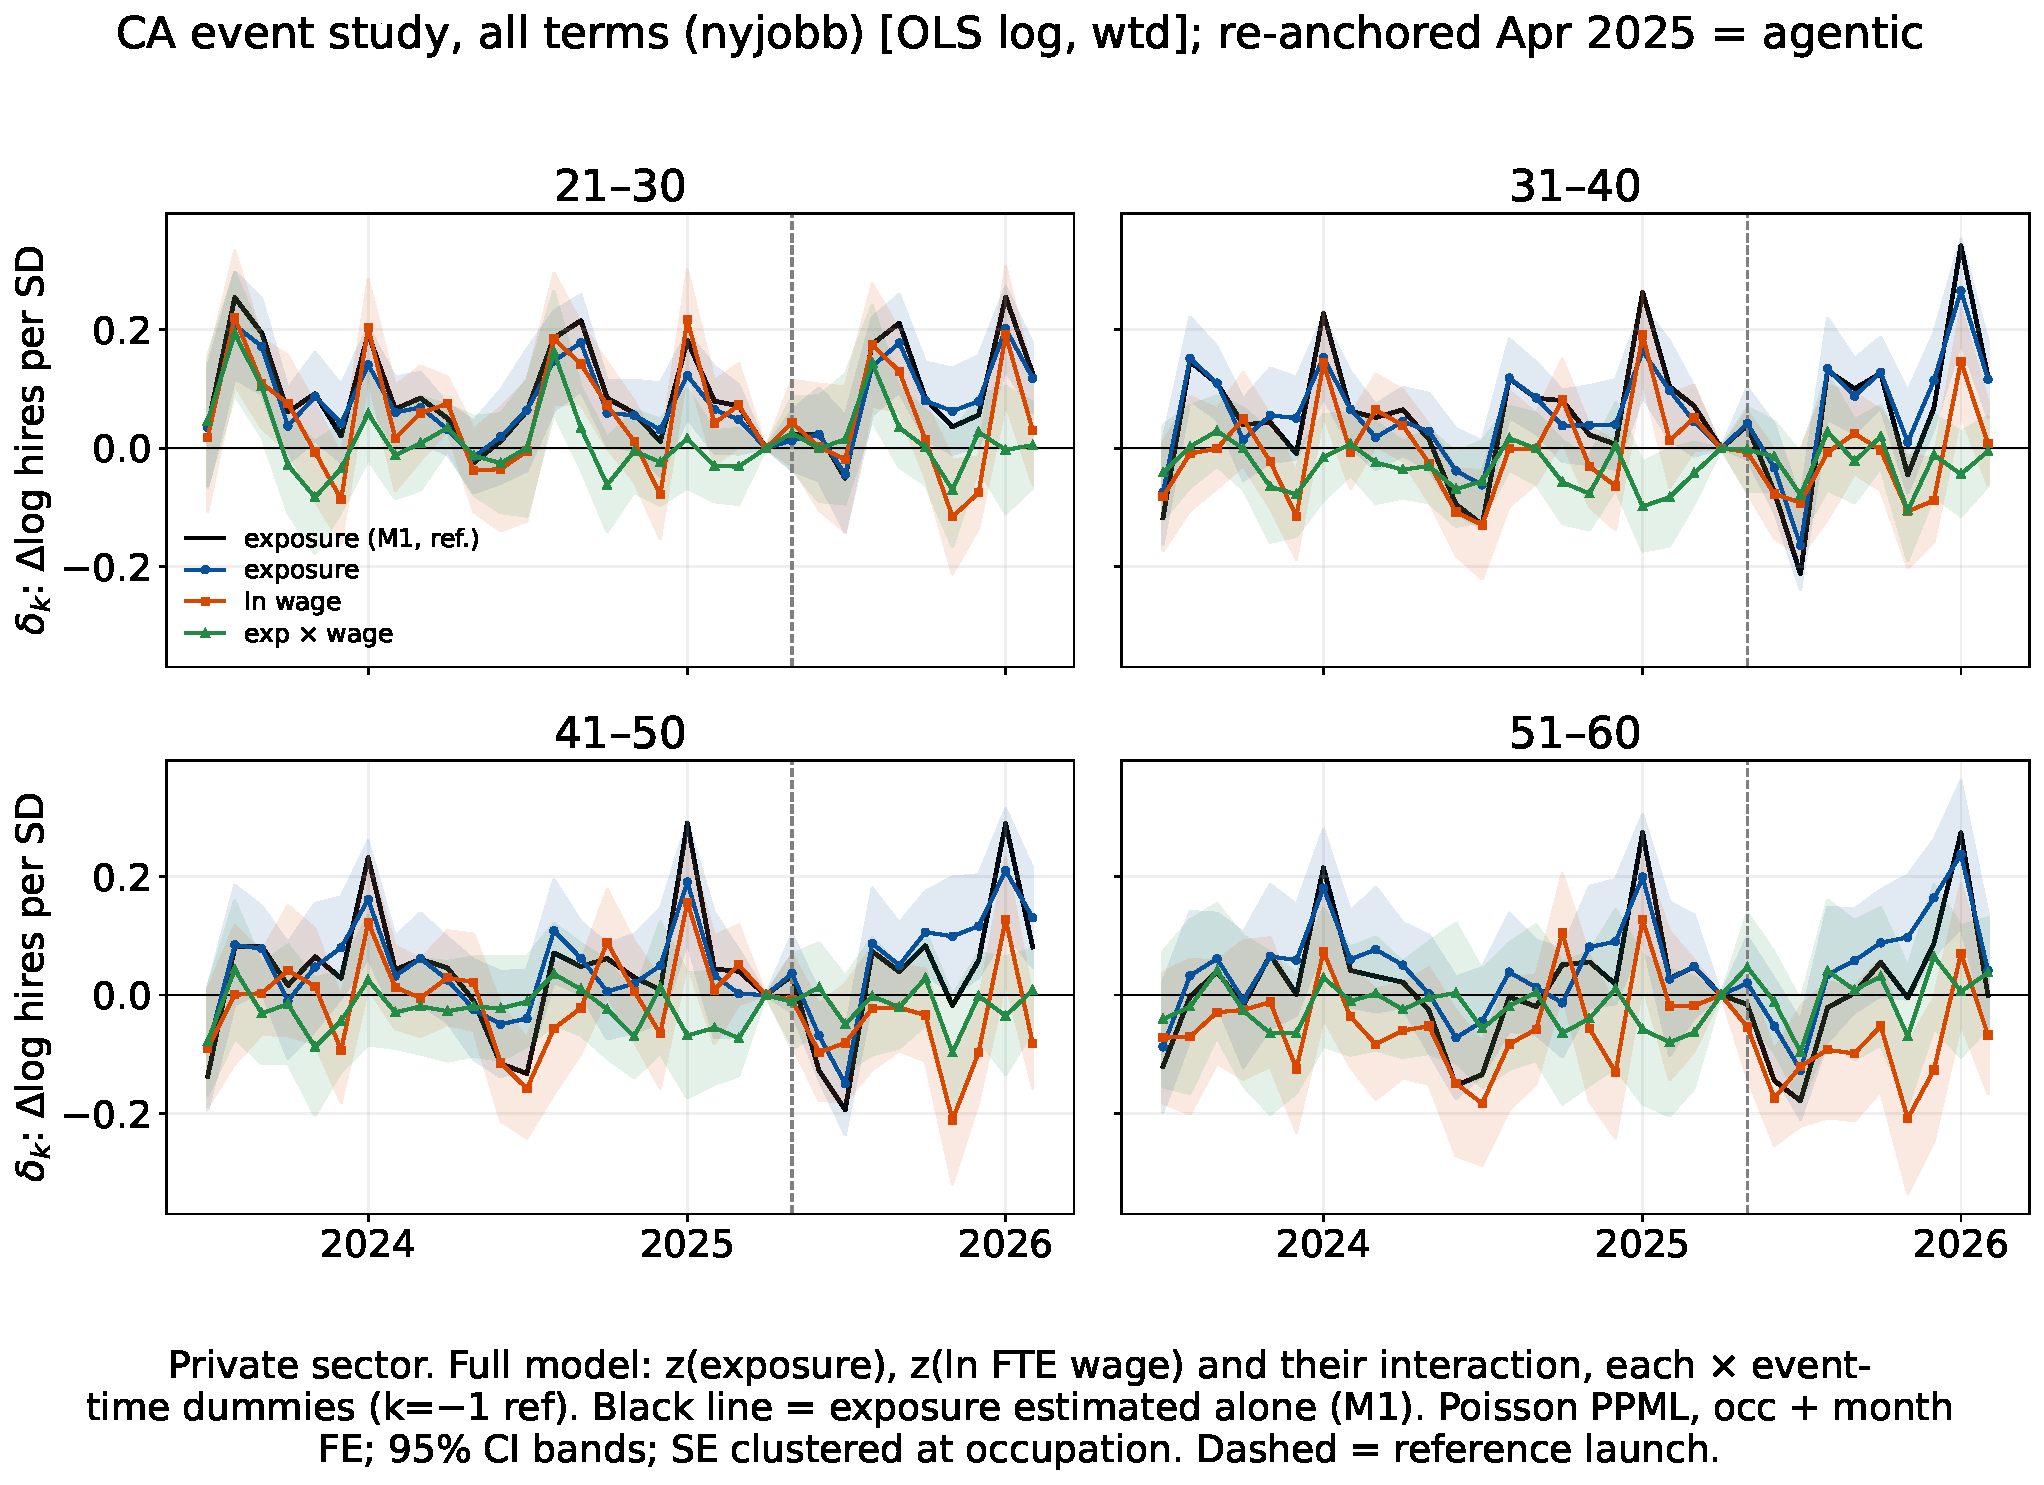
\includegraphics[width=\textwidth,height=0.42\textheight,keepaspectratio]{figure_ca_es_decade_agentic_stdexp_nyjobb_olslog.pdf}
  \caption{Log new hires (OLS, baseline-weighted): CA event study ---
           ChatGPT anchor (top), agentic anchor (bottom).}
\end{figure}

\clearpage
\subsection{Pooled post-treatment (DiD)}
\begin{table}[H]\centering
\caption{AI exposure, wage, and private-sector log new hires, by age group}
\label{tab:ca_did_combined_nyjobb_olslog}
\small
\begin{tabular}{lcccccc}
\toprule
 & \multicolumn{3}{c}{ChatGPT (ref.\ Oct 2022)} & \multicolumn{3}{c}{Agentic (ref.\ Apr 2025)} \\
\cmidrule(lr){2-4} \cmidrule(lr){5-7}
 & (1) & (2) & (3) & (4) & (5) & (6) \\
\midrule
\multicolumn{7}{@{}l}{\textit{Panel A: ages 21–30}} \\
Exposure $\times$ Post & -0.0465* &  & -0.0410 & +0.0941*** &  & +0.0850*** \\
 & (0.0251) &  & (0.0264) & (0.0231) &  & (0.0242) \\
ln wage $\times$ Post &  & -0.0353 & -0.0235 &  & +0.0613** & +0.0376 \\
 &  & (0.0215) & (0.0230) &  & (0.0270) & (0.0271) \\
Exp $\times$ wage $\times$ Post &  &  & -0.0155 &  &  & +0.0181 \\
 &  &  & (0.0311) &  &  & (0.0254) \\
\quad Observations & \multicolumn{3}{c}{16,781} & \multicolumn{3}{c}{10,229} \\
\quad Occupations & \multicolumn{3}{c}{363} & \multicolumn{3}{c}{360} \\
\midrule
\multicolumn{7}{@{}l}{\textit{Panel B: ages 31–40}} \\
Exposure $\times$ Post & -0.0279 &  & -0.0011 & +0.0596*** &  & +0.0703*** \\
 & (0.0249) &  & (0.0249) & (0.0207) &  & (0.0235) \\
ln wage $\times$ Post &  & -0.0540*** & -0.0532*** &  & +0.0157 & -0.0201 \\
 &  & (0.0207) & (0.0198) &  & (0.0236) & (0.0251) \\
Exp $\times$ wage $\times$ Post &  &  & -0.0636** &  &  & -0.0232 \\
 &  &  & (0.0311) &  &  & (0.0216) \\
\quad Observations & \multicolumn{3}{c}{16,618} & \multicolumn{3}{c}{10,097} \\
\quad Occupations & \multicolumn{3}{c}{367} & \multicolumn{3}{c}{359} \\
\midrule
\multicolumn{7}{@{}l}{\textit{Panel C: ages 41–50}} \\
Exposure $\times$ Post & -0.0388 &  & +0.0010 & +0.0321 &  & +0.0618** \\
 & (0.0247) &  & (0.0244) & (0.0204) &  & (0.0294) \\
ln wage $\times$ Post &  & -0.0717*** & -0.0723*** &  & -0.0188 & -0.0522* \\
 &  & (0.0220) & (0.0237) &  & (0.0248) & (0.0315) \\
Exp $\times$ wage $\times$ Post &  &  & -0.0320 &  &  & -0.0166 \\
 &  &  & (0.0347) &  &  & (0.0285) \\
\quad Observations & \multicolumn{3}{c}{15,847} & \multicolumn{3}{c}{9,653} \\
\quad Occupations & \multicolumn{3}{c}{364} & \multicolumn{3}{c}{359} \\
\midrule
\multicolumn{7}{@{}l}{\textit{Panel D: ages 51–60}} \\
Exposure $\times$ Post & -0.0405 &  & +0.0001 & +0.0057 &  & +0.0564* \\
 & (0.0258) &  & (0.0272) & (0.0264) &  & (0.0341) \\
ln wage $\times$ Post &  & -0.0768*** & -0.0767** &  & -0.0637* & -0.0923** \\
 &  & (0.0276) & (0.0316) &  & (0.0353) & (0.0413) \\
Exp $\times$ wage $\times$ Post &  &  & -0.0061 &  &  & +0.0065 \\
 &  &  & (0.0317) &  &  & (0.0397) \\
\quad Observations & \multicolumn{3}{c}{14,525} & \multicolumn{3}{c}{8,910} \\
\quad Occupations & \multicolumn{3}{c}{361} & \multicolumn{3}{c}{352} \\
\midrule
Occupation FE & Yes & Yes & Yes & Yes & Yes & Yes \\
Month FE & Yes & Yes & Yes & Yes & Yes & Yes \\
\bottomrule
\end{tabular}
\begin{minipage}{\linewidth}\vspace{2pt}\footnotesize
\emph{Notes:} OLS on log new hires, weighted by baseline (pre-period) new hires (zero cells dropped) (cell-level log new hires, private sector). Columns (1)--(3): ChatGPT window (Oct 2022 $=k{=}{-}1$, through 2025m4); (4)--(6): agentic (Apr 2025 $=k{=}{-}1$, from 2023m7). Each coefficient is the average post-period effect relative to the reference month ($k{=}{-}1$); each pre-period month enters as a separate control. M1 = exposure only, M2 = ln wage only, M3 = both $+$ interaction. Treatments standardized: $z(\text{exp})$ = Eloundou $\beta$ (pooled), $z(\text{lnw})$ = ln full-time-equivalent wage within age group. Occupation and month fixed effects in all columns; SE clustered at occupation in parentheses; coefficients are $\Delta\log$ per 1 SD. $^{*}p<0.10$, $^{**}p<0.05$, $^{***}p<0.01$.
\end{minipage}
\end{table}

% =====================================================================
\clearpage
\section{Firm-FE event studies (Poisson PPML, within-firm)}

\noindent
Sections 1--4 fit the CA model on the microdata.no aggregate cell panel
(occupation $+$ month FE). This chapter replicates the same specification on
the secure-server individual-level firm panel and substitutes the
Brynjolfsson--Chandar--Chen (BCC) eq.\ 4.1 fixed-effect structure: firm
$\times$ occupation $+$ firm $\times$ month. The firm $\times$ month FE
absorbs every firm-level time shock (sector, geography, demand, etc.); the
firm $\times$ occupation FE absorbs firm-specific occupation baselines. The
treatment paths $i(k, z_{\text{exp}}) + i(k, z_{\text{wage}})
+ i(k, z_{\text{exp$\times$wage}})$ survive the FE because they vary by
occupation $\times$ time within firm-month --- BCC's within-firm
differential-exposure identification.
\medskip

\noindent
The exposure-cell is \textbf{firm $\times$ occupation}, the
continuous-treatment-faithful spec: the cell coincides with the level at
which $z_{\text{exp}}/z_{\text{wage}}$ vary, so it absorbs firm-occupation
baselines (subsuming a plain occupation FE). It identifies off firms with
$\geq 2$ occupations in the same age-month. This is the within-firm
robustness check that the cell-level paths in \S\S1--4 are not driven by
between-firm sorting on occupation.
\medskip

\noindent
Sample: \texttt{in\_headline\_priv} (private sector, $\geq 20$ workers in
the age window per active month), 21--30 / 31--40 / 41--50 / 51--60 decade
bins. SE clustered at foretak. The observation counts reported in the
tables are the fepois pre-fit sample size (after singleton-FE and
all-zero outcome drops that fepois removes before estimation), so they
are smaller than the raw panel counts in the firm $\times$ month panel.
$z_{\text{exp}}$ is the Eloundou GPT-4 $\beta$ pooled across occupations,
identical to \S\S1--4. $z_{\text{wage}}$ is computed natively on the
secure private sample (pre-ChatGPT employment-weighted log FTE wage
per occupation $\times$ age, z-scored within age), so the wage object
is the secure-sample analogue of \S1's wage rather than the identical
vector.

\subsection{Employment (count), firm $\times$ occupation FE}
\begin{figure}[H]\centering
  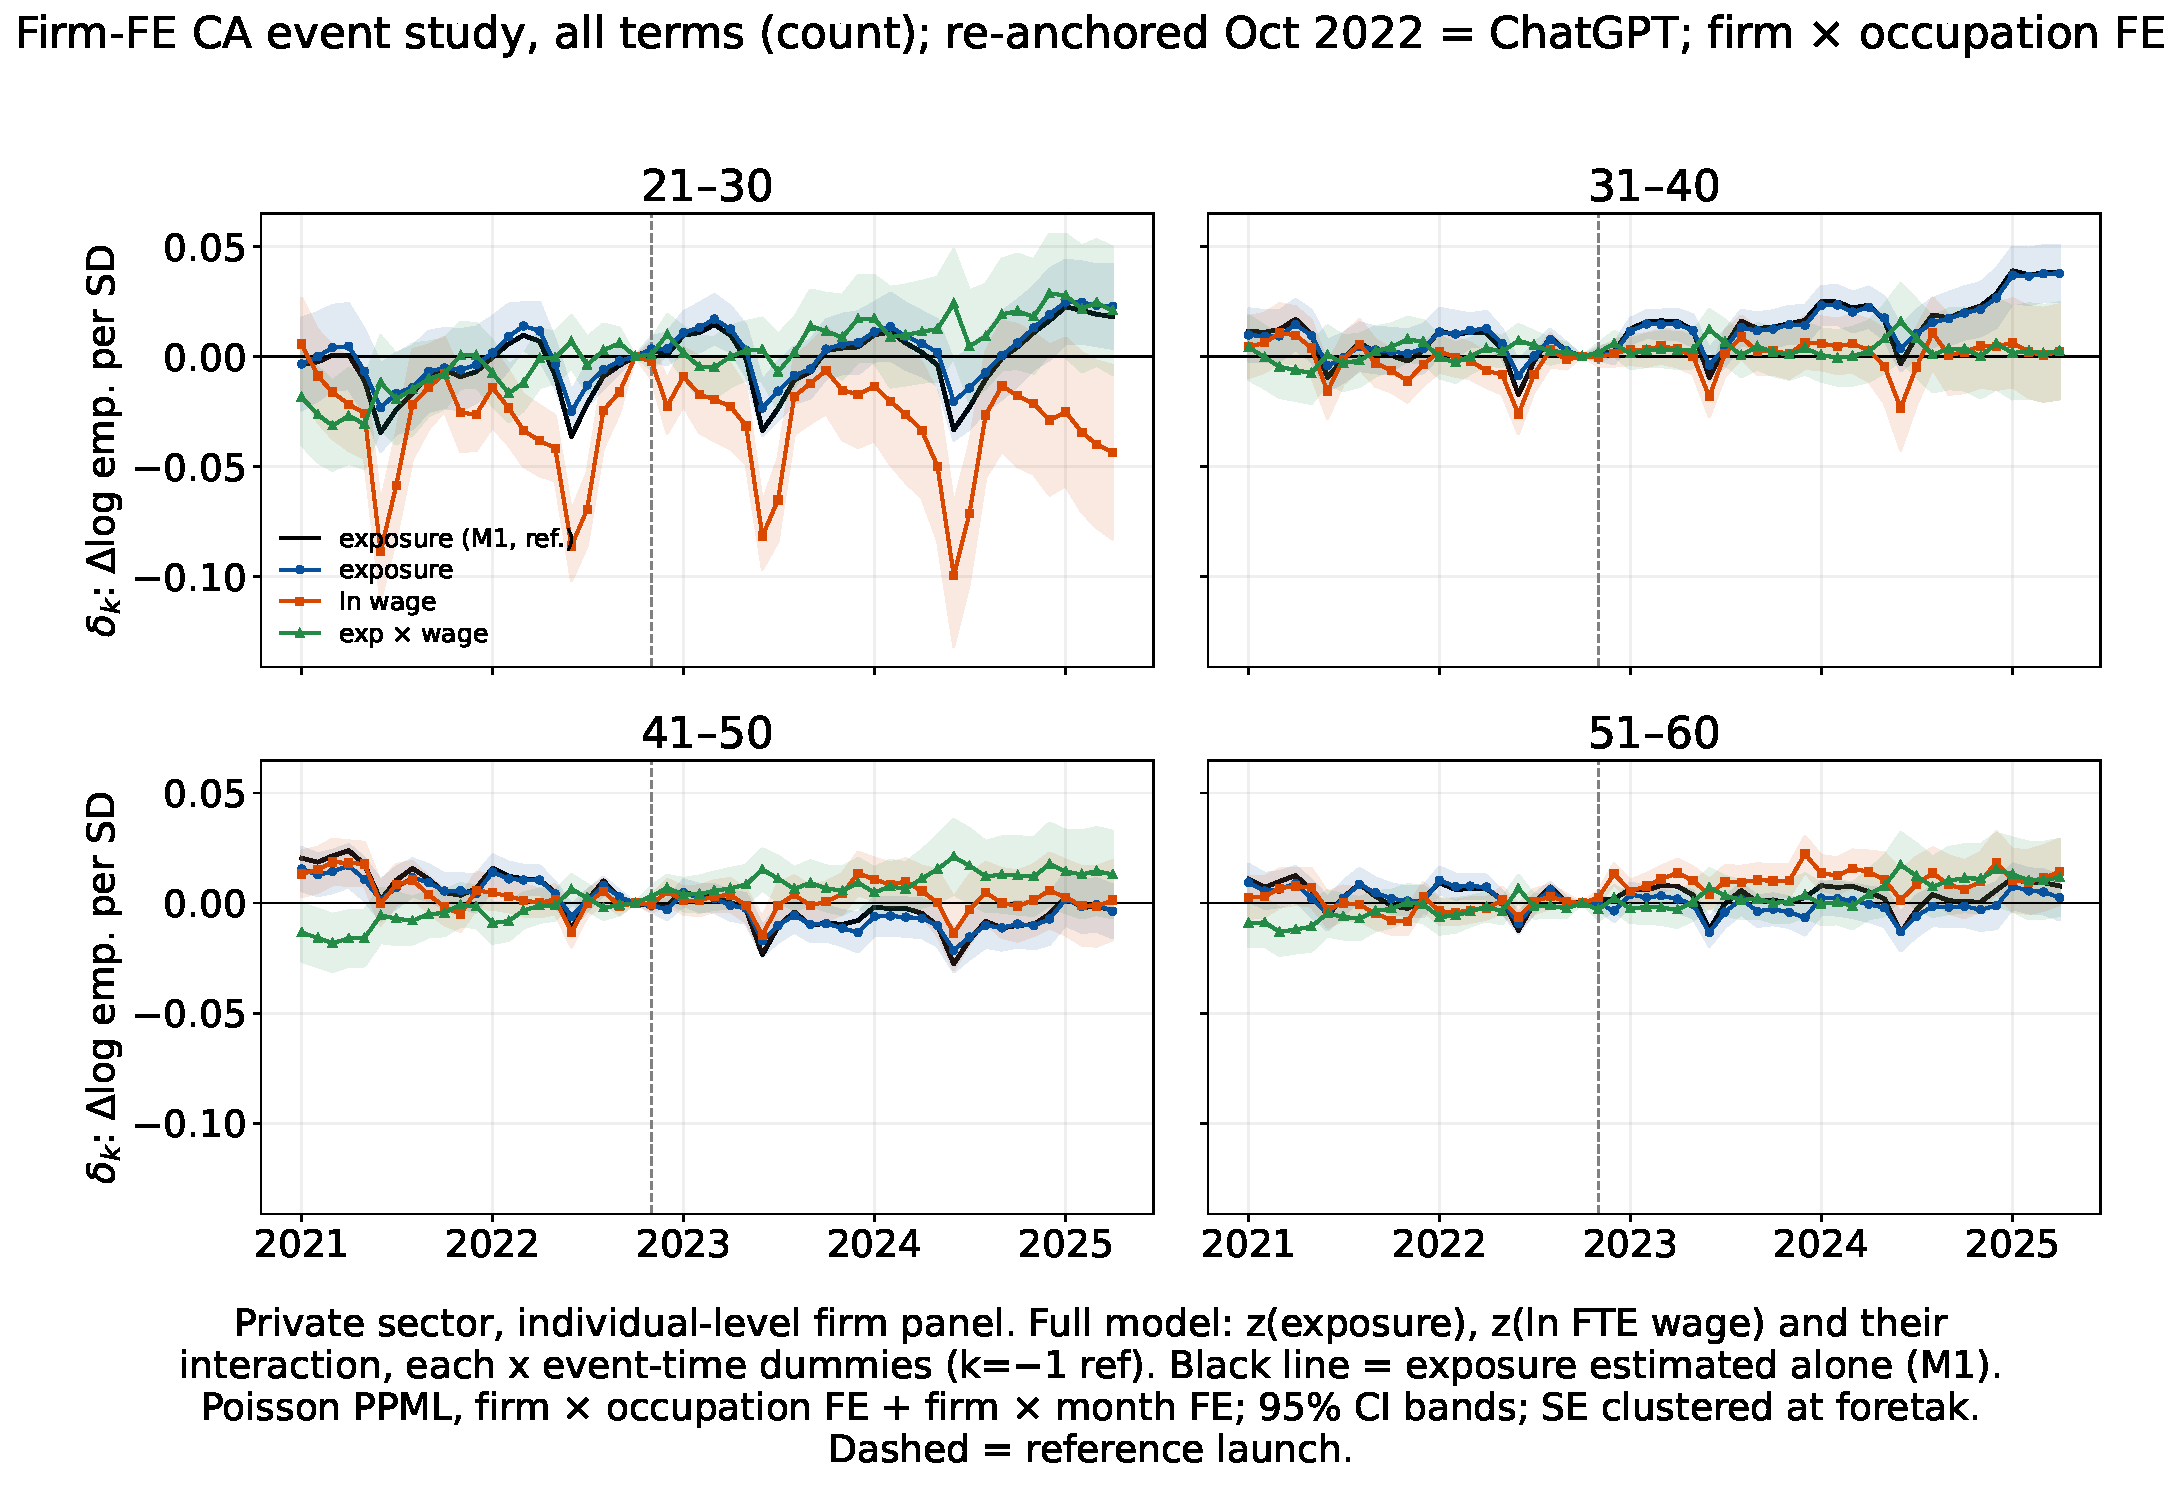
\includegraphics[width=\textwidth,height=0.42\textheight,keepaspectratio]{figure_ca_es_firmfe_grid_count_occ.pdf}\\[4pt]
  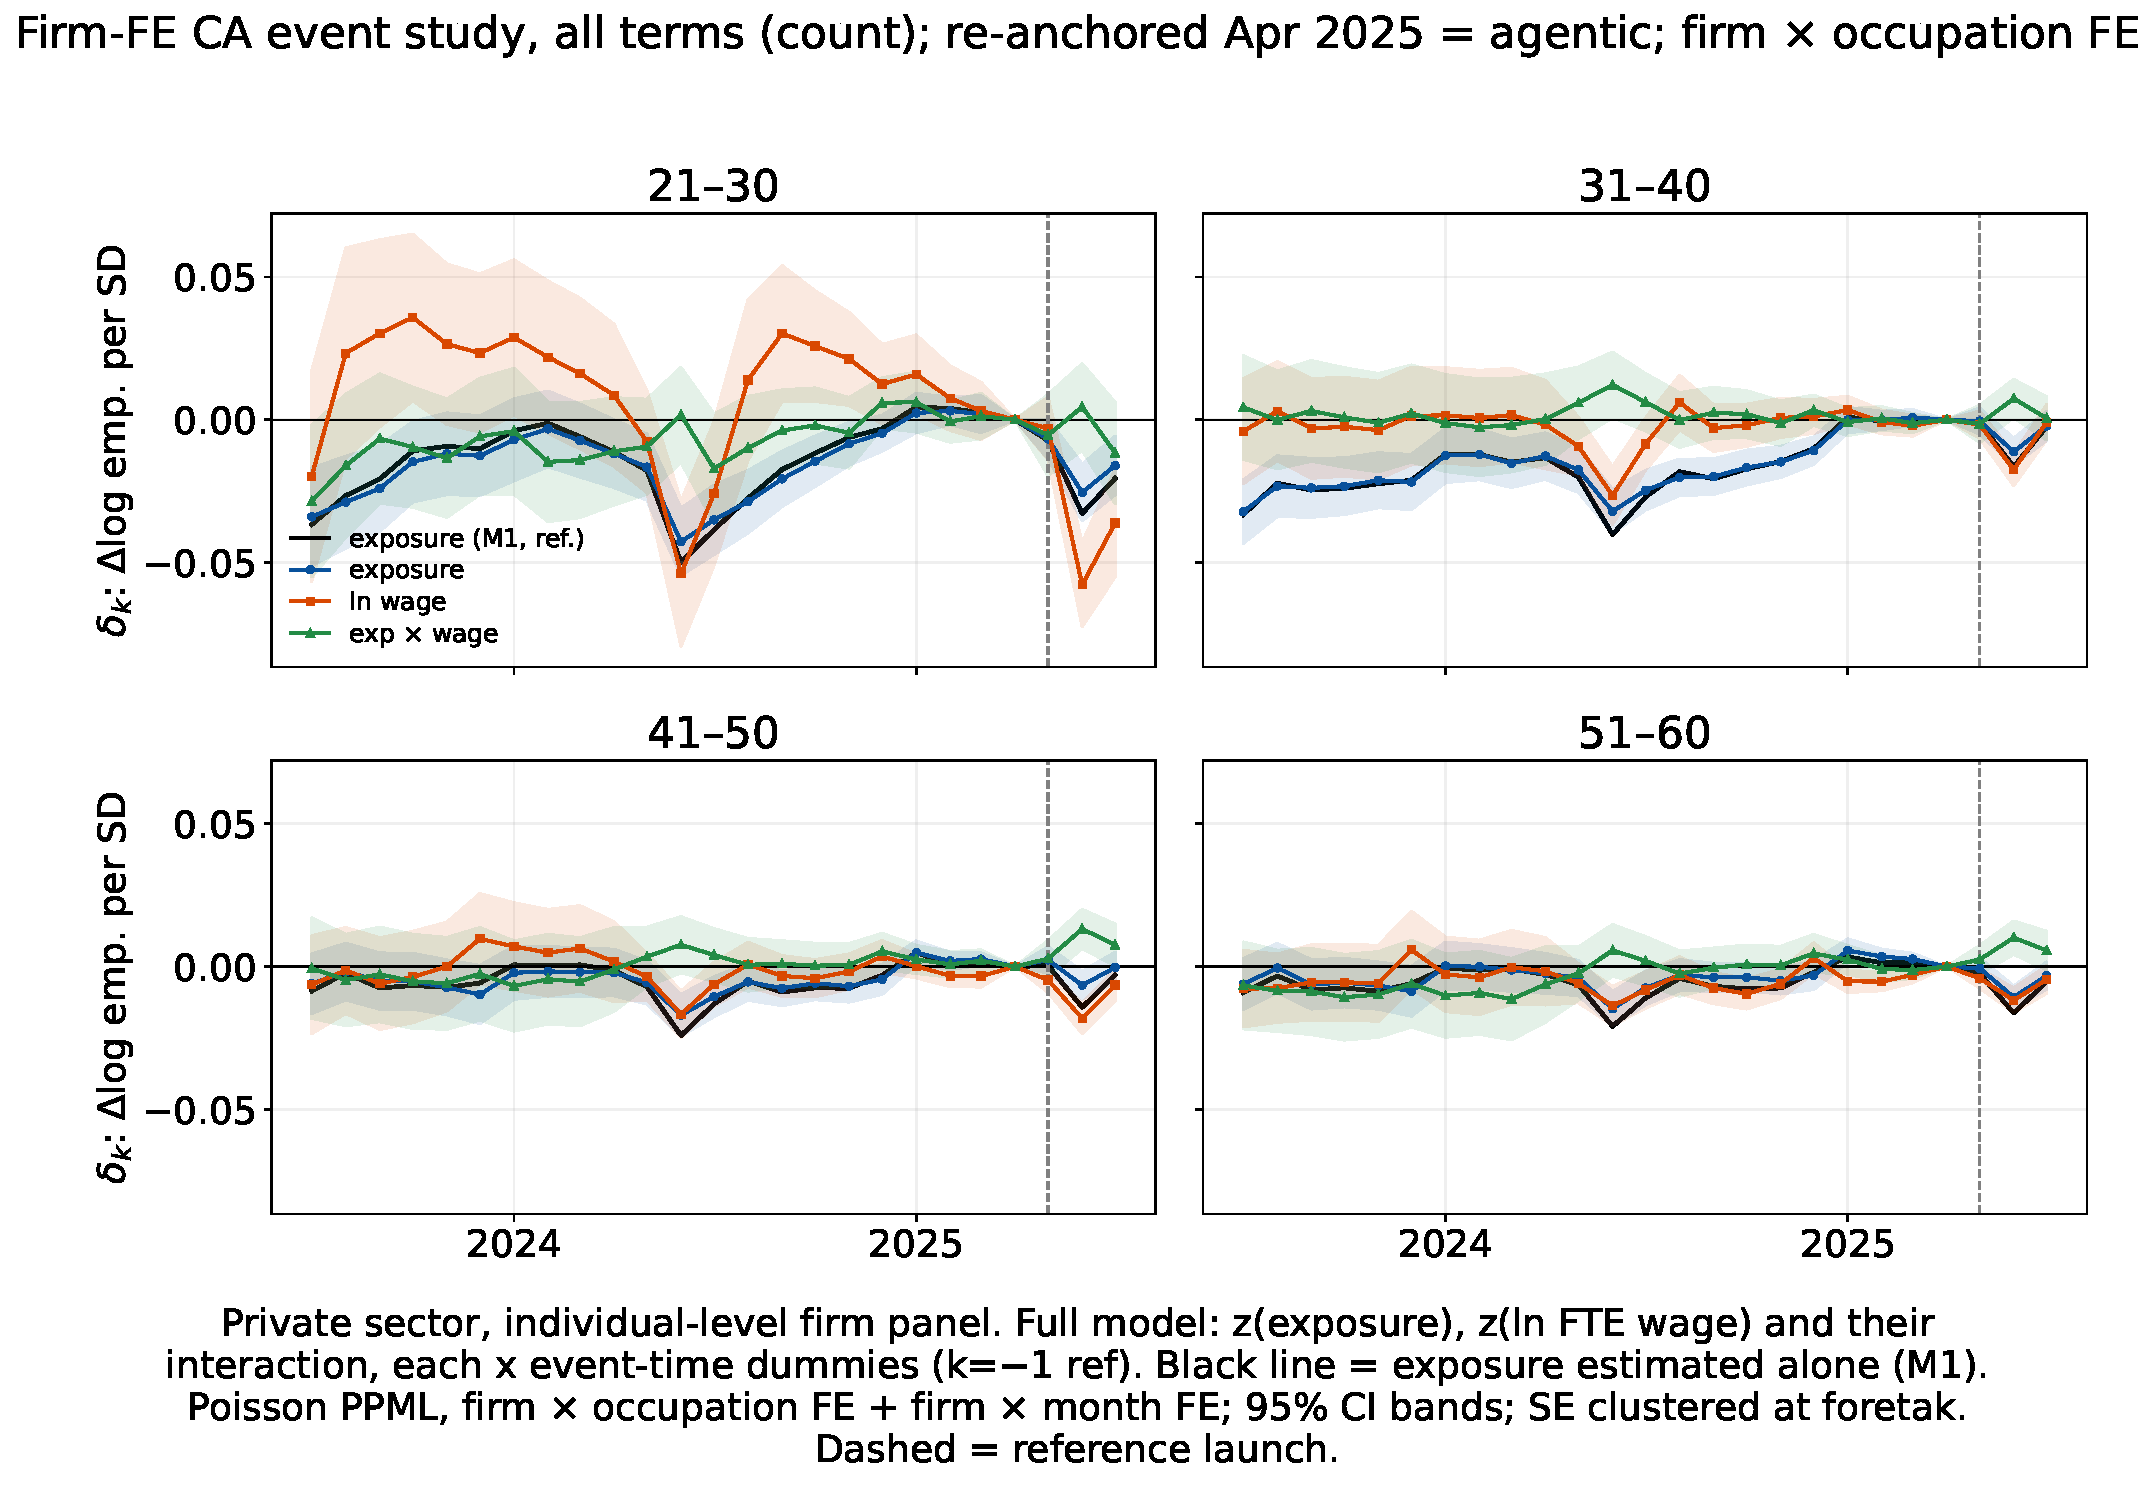
\includegraphics[width=\textwidth,height=0.42\textheight,keepaspectratio]{figure_ca_es_firmfe_decade_agentic_count_occ.pdf}
  \caption{Firm-FE CA event study, employment (count), firm $\times$
           occupation cell --- ChatGPT anchor (top), agentic anchor (bottom).}
\end{figure}

\clearpage
\subsection{New hires (nyjobb), firm $\times$ occupation FE}
\begin{figure}[H]\centering
  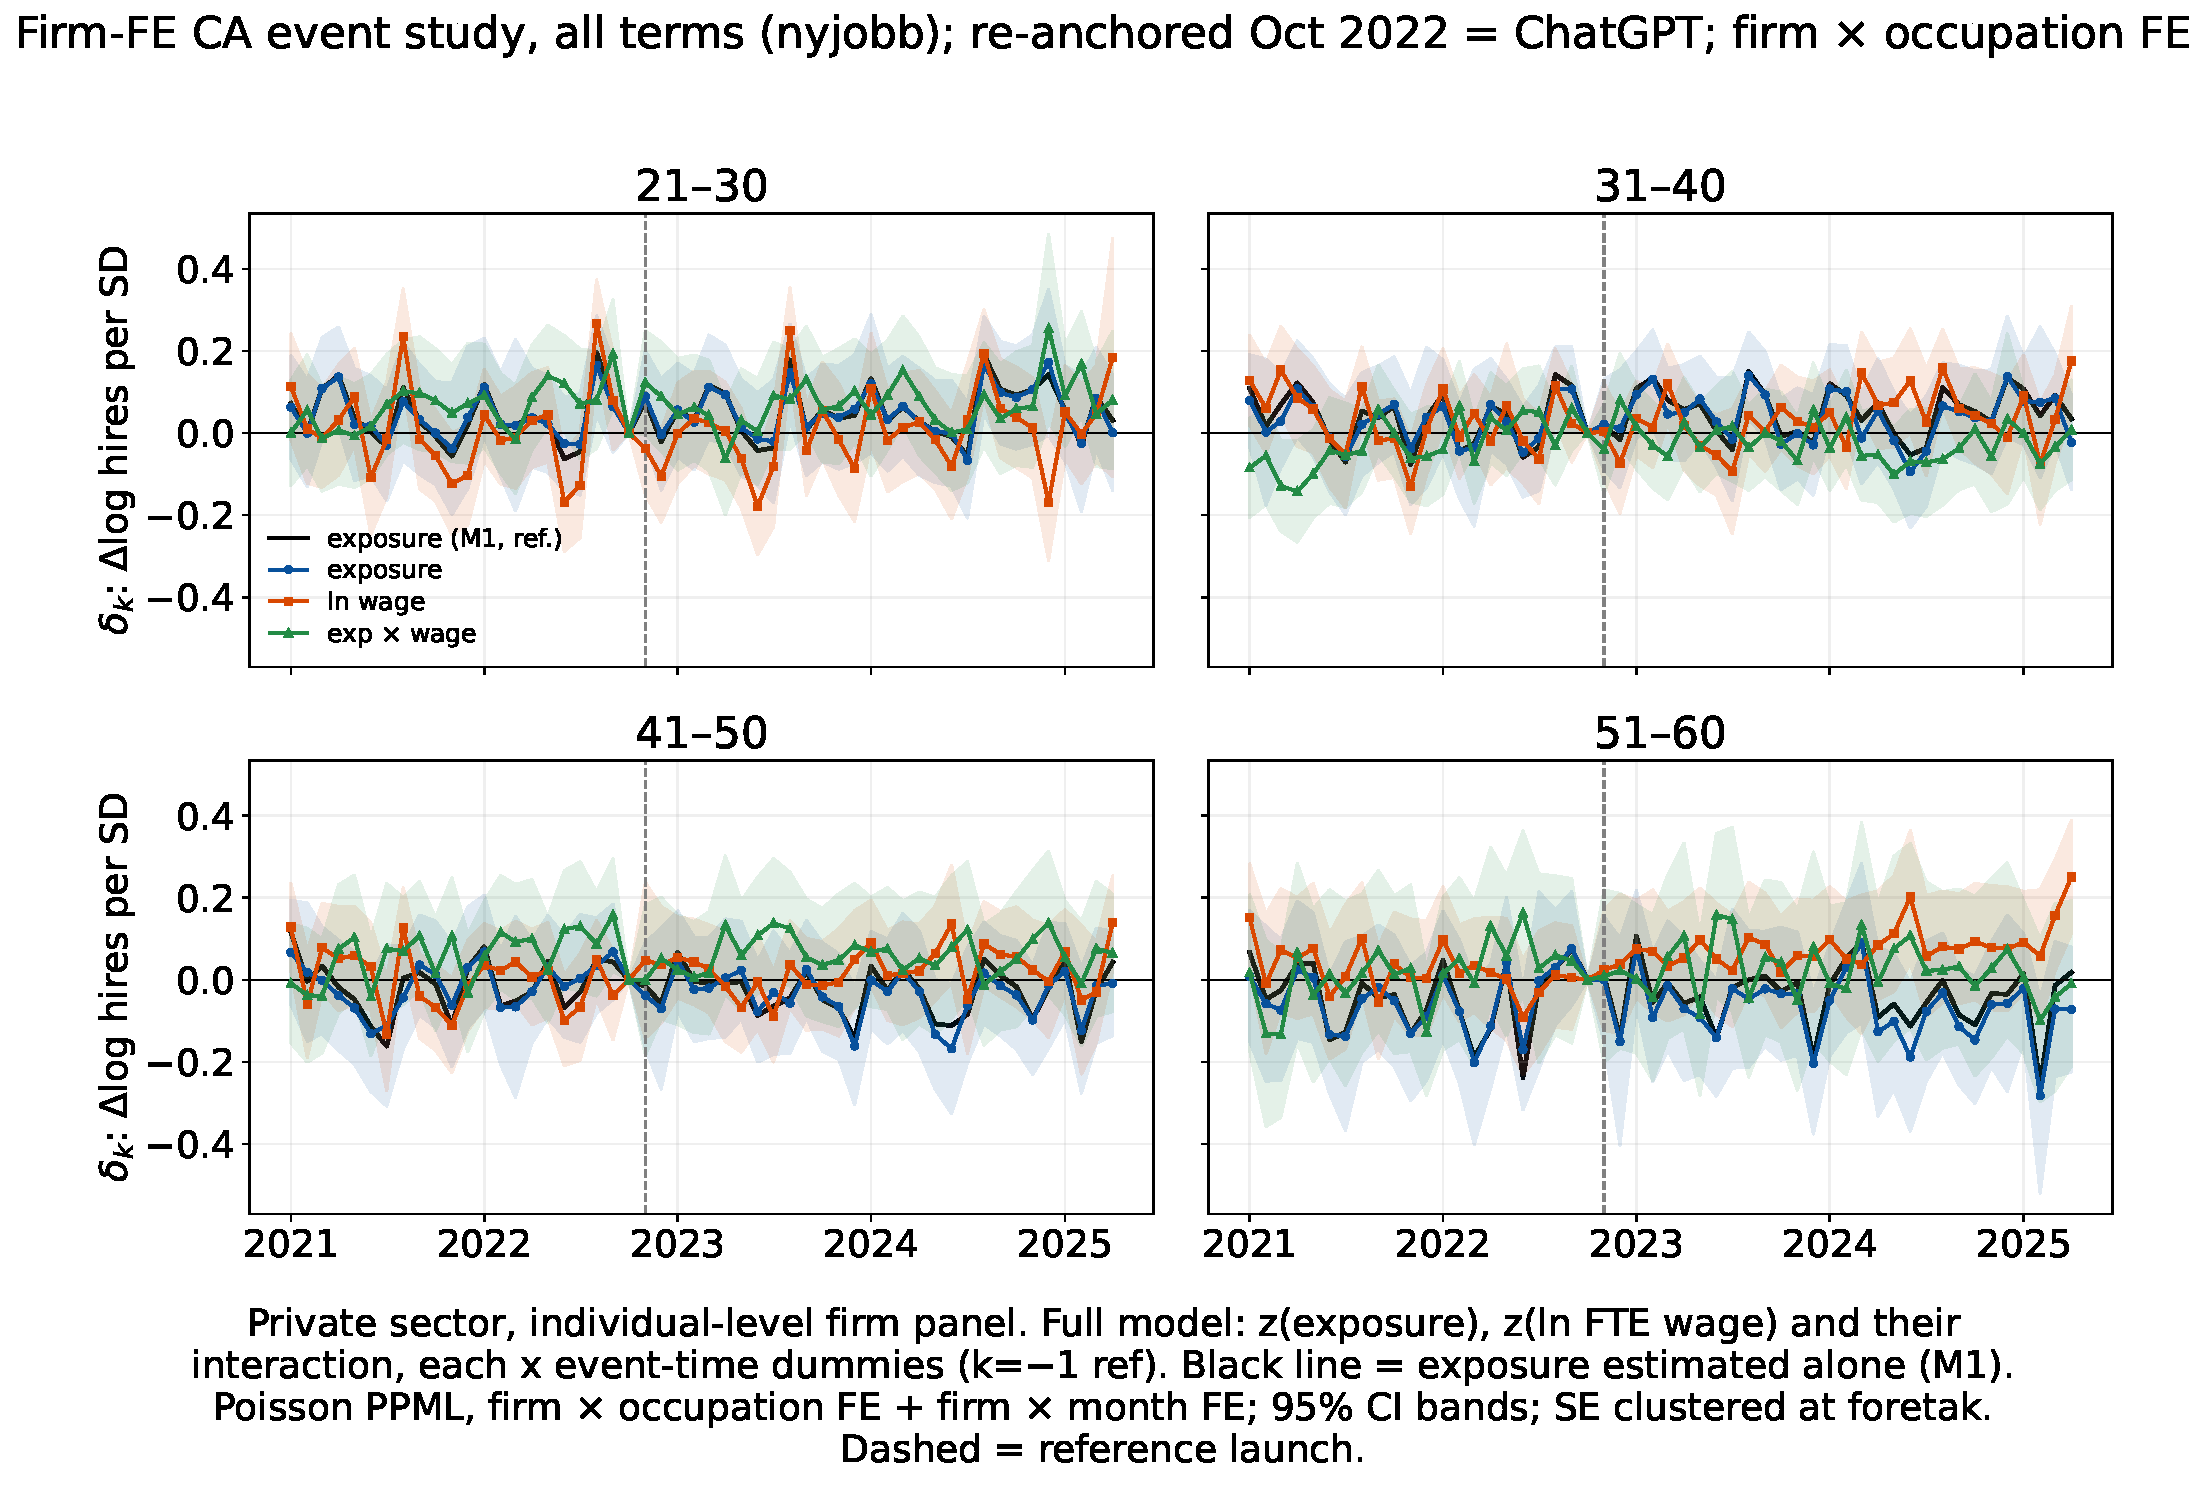
\includegraphics[width=\textwidth,height=0.42\textheight,keepaspectratio]{figure_ca_es_firmfe_grid_nyjobb_occ.pdf}\\[4pt]
  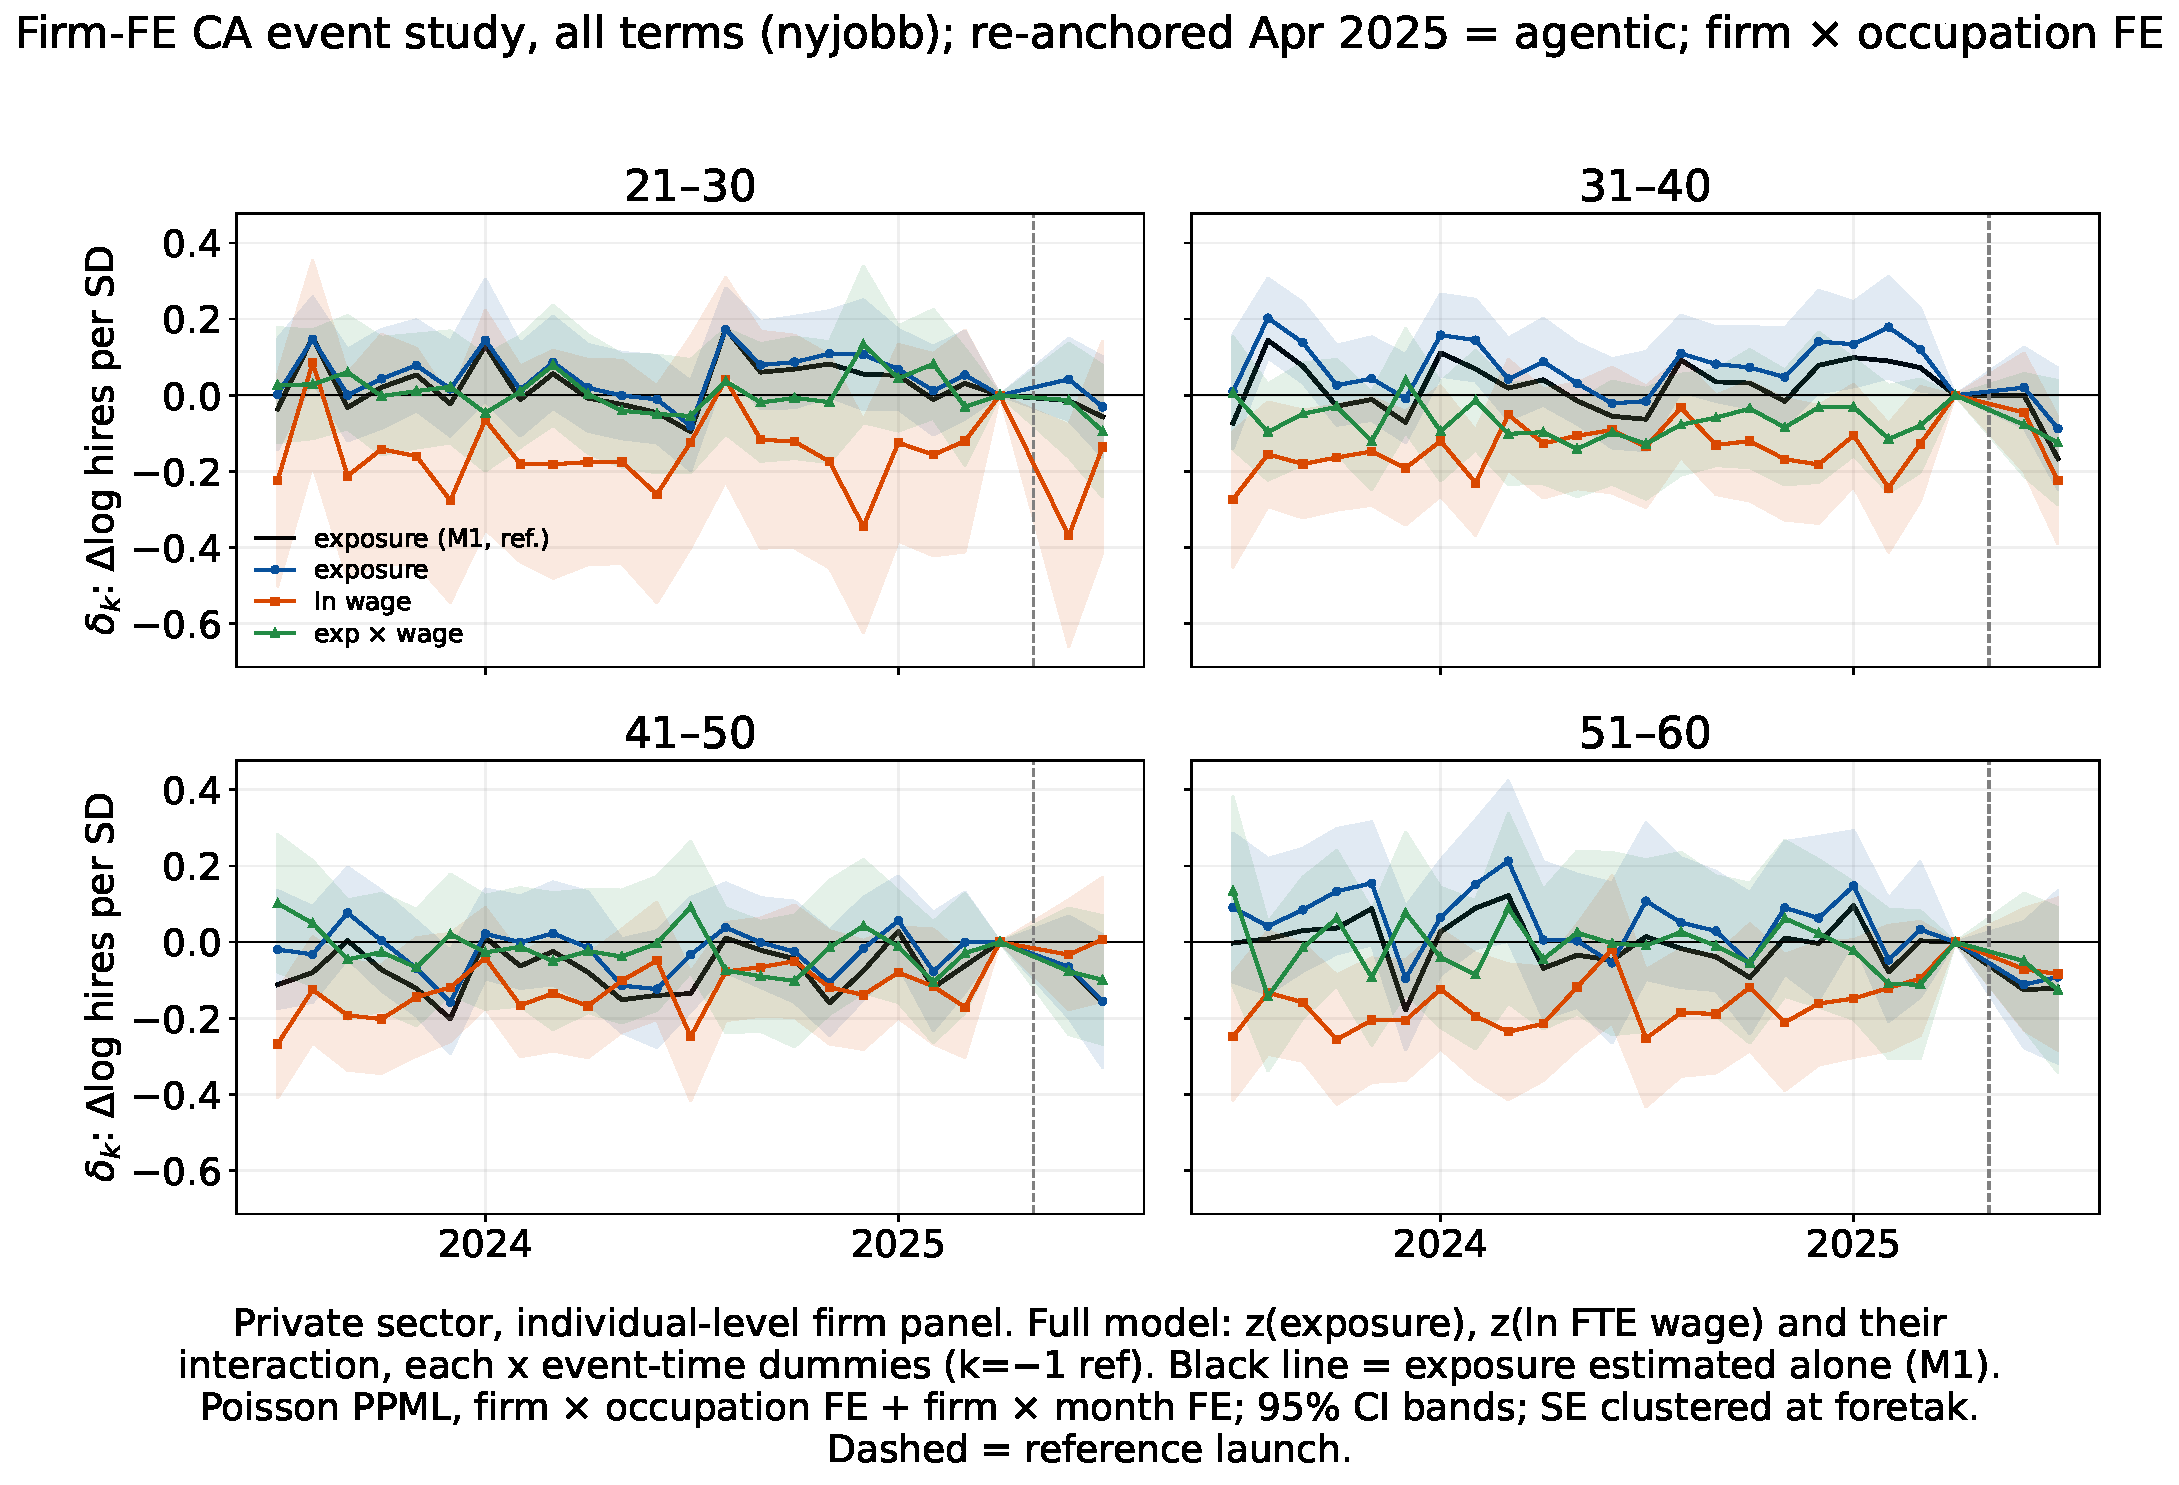
\includegraphics[width=\textwidth,height=0.42\textheight,keepaspectratio]{figure_ca_es_firmfe_decade_agentic_nyjobb_occ.pdf}
  \caption{Firm-FE CA event study, new hires (nyjobb), firm $\times$
           occupation cell --- ChatGPT anchor (top), agentic anchor (bottom).}
\end{figure}

% =====================================================================
\clearpage
\section{Firm-FE pooled DiD (Poisson PPML, within-firm)}

\noindent
Pooled post-treatment analogue of Section 5, mirroring Section 2's table
format. Each pre-period month enters as its own control level; all post
months collapse to ``POST'' with the reference month ($k=-1$) omitted, so
each POST coefficient is the average post-period effect relative to the
reference month. Three nested specifications per (timing, age) cell:
\begin{itemize}\setlength{\itemsep}{1pt}
  \item \textbf{M1} (\emph{exp}): $z_{\text{exp}} \cdot \text{Post}$ only.
  \item \textbf{M2} (\emph{wage}): $z_{\text{wage}} \cdot \text{Post}$ only.
  \item \textbf{M3} (\emph{full}): $z_{\text{exp}}\,\text{Post} +
        z_{\text{wage}}\,\text{Post} + (z_{\text{exp}} z_{\text{wage}})
        \,\text{Post}$.
\end{itemize}

\subsection{Employment (count), firm $\times$ occupation FE}
\begin{table}[H]\centering
\caption{Firm-FE CA pooled DiD on private-sector employment headcount, by age group (firm-occupation cell)}
\label{tab:ca_did_firmfe_combined_count_occ}
\small
\begin{tabular}{lcccccc}
\toprule
 & \multicolumn{3}{c}{ChatGPT (ref.\ Oct 2022)} & \multicolumn{3}{c}{Agentic (ref.\ Apr 2025)} \\
\cmidrule(lr){2-4} \cmidrule(lr){5-7}
 & (1) & (2) & (3) & (4) & (5) & (6) \\
\midrule
\multicolumn{7}{@{}l}{\textit{Panel A: ages 21–30}} \\
Exposure $\times$ Post & +0.0011 &  & +0.0048 & -0.0206*** &  & -0.0164*** \\
 & (0.0061) &  & (0.0059) & (0.0038) &  & (0.0039) \\
ln wage $\times$ Post &  & -0.0296*** & -0.0309*** &  & -0.0364*** & -0.0335*** \\
 &  & (0.0107) & (0.0107) &  & (0.0062) & (0.0064) \\
Exp $\times$ wage $\times$ Post &  &  & +0.0111 &  &  & -0.0036 \\
 &  &  & (0.0083) &  &  & (0.0074) \\
\quad Observations & \multicolumn{3}{c}{4,224,298} & \multicolumn{3}{c}{1,662,029} \\
\quad Foretak (clusters) & \multicolumn{3}{c}{20,556} & \multicolumn{3}{c}{17,426} \\
\midrule
\multicolumn{7}{@{}l}{\textit{Panel B: ages 31–40}} \\
Exposure $\times$ Post & +0.0169*** &  & +0.0164*** & -0.0068*** &  & -0.0047** \\
 & (0.0037) &  & (0.0038) & (0.0020) &  & (0.0022) \\
ln wage $\times$ Post &  & +0.0086* & +0.0010 &  & -0.0081*** & -0.0069*** \\
 &  & (0.0048) & (0.0056) &  & (0.0019) & (0.0024) \\
Exp $\times$ wage $\times$ Post &  &  & +0.0038 &  &  & +0.0023 \\
 &  &  & (0.0056) &  &  & (0.0033) \\
\quad Observations & \multicolumn{3}{c}{5,367,725} & \multicolumn{3}{c}{2,187,096} \\
\quad Foretak (clusters) & \multicolumn{3}{c}{20,607} & \multicolumn{3}{c}{17,457} \\
\midrule
\multicolumn{7}{@{}l}{\textit{Panel C: ages 41–50}} \\
Exposure $\times$ Post & -0.0061** &  & -0.0066* & -0.0057*** &  & -0.0016 \\
 & (0.0031) &  & (0.0036) & (0.0019) &  & (0.0024) \\
ln wage $\times$ Post &  & +0.0020 & +0.0015 &  & -0.0083*** & -0.0099*** \\
 &  & (0.0034) & (0.0046) &  & (0.0017) & (0.0023) \\
Exp $\times$ wage $\times$ Post &  &  & +0.0103** &  &  & +0.0080** \\
 &  &  & (0.0052) &  &  & (0.0032) \\
\quad Observations & \multicolumn{3}{c}{5,498,699} & \multicolumn{3}{c}{2,229,602} \\
\quad Foretak (clusters) & \multicolumn{3}{c}{20,482} & \multicolumn{3}{c}{17,361} \\
\midrule
\multicolumn{7}{@{}l}{\textit{Panel D: ages 51–60}} \\
Exposure $\times$ Post & +0.0031 &  & -0.0010 & -0.0081*** &  & -0.0049** \\
 & (0.0028) &  & (0.0032) & (0.0015) &  & (0.0019) \\
ln wage $\times$ Post &  & +0.0119*** & +0.0106*** &  & -0.0066*** & -0.0069*** \\
 &  & (0.0027) & (0.0037) &  & (0.0013) & (0.0019) \\
Exp $\times$ wage $\times$ Post &  &  & +0.0050 &  &  & +0.0062** \\
 &  &  & (0.0046) &  &  & (0.0027) \\
\quad Observations & \multicolumn{3}{c}{4,940,889} & \multicolumn{3}{c}{2,104,661} \\
\quad Foretak (clusters) & \multicolumn{3}{c}{19,992} & \multicolumn{3}{c}{16,980} \\
\midrule
firm $\times$ occupation FE & Yes & Yes & Yes & Yes & Yes & Yes \\
Firm $\times$ month FE & Yes & Yes & Yes & Yes & Yes & Yes \\
\bottomrule
\end{tabular}
\begin{minipage}{\linewidth}\vspace{2pt}\footnotesize
\emph{Notes:} Poisson PPML (\texttt{fixest::fepois}) on the individual-level firm panel (private sector, \texttt{in\_headline\_priv}). Outcome: cell-level employment headcount summed within (foretak, occupation, age, month). Fixed effects: firm $\times$ occupation $+$ firm $\times$ month (BCC eq.\ 4.1 within-firm time-shock control). Columns (1)--(3): ChatGPT window (Oct 2022 $=k{=}{-}1$, through 2025m4); (4)--(6): agentic (Apr 2025 $=k{=}{-}1$, from 2023m7). Each coefficient is the average post-period effect relative to the reference month ($k{=}{-}1$); each pre-period month enters as a separate control. M1 = exposure only, M2 = ln wage only, M3 = both $+$ interaction. Treatments standardized: $z(\text{exp})$ = Eloundou $\beta$ (pooled across occupations), $z(\text{lnw})$ = ln full-time-equivalent wage within age group (pre-ChatGPT, native to the secure private sample). SE clustered at foretak in parentheses; coefficients are $\Delta\log$ per 1 SD. $^{*}p<0.10$, $^{**}p<0.05$, $^{***}p<0.01$.
\end{minipage}
\end{table}

\clearpage
\subsection{New hires (nyjobb), firm $\times$ occupation FE}
\begin{table}[H]\centering
\caption{Firm-FE CA pooled DiD on private-sector new hires = round(count $\times$ ny\_jobb), by age group (firm-occupation cell)}
\label{tab:ca_did_firmfe_combined_nyjobb_occ}
\small
\begin{tabular}{lcccccc}
\toprule
 & \multicolumn{3}{c}{ChatGPT (ref.\ Oct 2022)} & \multicolumn{3}{c}{Agentic (ref.\ Apr 2025)} \\
\cmidrule(lr){2-4} \cmidrule(lr){5-7}
 & (1) & (2) & (3) & (4) & (5) & (6) \\
\midrule
\multicolumn{7}{@{}l}{\textit{Panel A: ages 21–30}} \\
Exposure $\times$ Post & +0.0588 &  & +0.0559 & -0.0292 &  & +0.0121 \\
 & (0.0553) &  & (0.0540) & (0.0437) &  & (0.0526) \\
ln wage $\times$ Post &  & +0.0356 & +0.0166 &  & -0.2826* & -0.2853** \\
 &  & (0.0460) & (0.0450) &  & (0.1443) & (0.1443) \\
Exp $\times$ wage $\times$ Post &  &  & +0.0741 &  &  & -0.0484 \\
 &  &  & (0.0546) &  &  & (0.0733) \\
\quad Observations & \multicolumn{3}{c}{904,733} & \multicolumn{3}{c}{281,549} \\
\quad Foretak (clusters) & \multicolumn{3}{c}{20,556} & \multicolumn{3}{c}{17,426} \\
\midrule
\multicolumn{7}{@{}l}{\textit{Panel B: ages 31–40}} \\
Exposure $\times$ Post & +0.0581 &  & +0.0480 & -0.0655 &  & -0.0225 \\
 & (0.0472) &  & (0.0464) & (0.0503) &  & (0.0524) \\
ln wage $\times$ Post &  & +0.0483 & +0.0344 &  & -0.1397** & -0.1097 \\
 &  & (0.0390) & (0.0370) &  & (0.0664) & (0.0730) \\
Exp $\times$ wage $\times$ Post &  &  & -0.0174 &  &  & -0.1003 \\
 &  &  & (0.0404) &  &  & (0.0637) \\
\quad Observations & \multicolumn{3}{c}{918,685} & \multicolumn{3}{c}{273,260} \\
\quad Foretak (clusters) & \multicolumn{3}{c}{20,607} & \multicolumn{3}{c}{17,457} \\
\midrule
\multicolumn{7}{@{}l}{\textit{Panel C: ages 41–50}} \\
Exposure $\times$ Post & -0.0224 &  & -0.0312 & -0.1044* &  & -0.1030 \\
 & (0.0484) &  & (0.0507) & (0.0588) &  & (0.0629) \\
ln wage $\times$ Post &  & +0.0331 & +0.0273 &  & -0.0694 & -0.0138 \\
 &  & (0.0413) & (0.0393) &  & (0.0616) & (0.0674) \\
Exp $\times$ wage $\times$ Post &  &  & +0.0575 &  &  & -0.0921 \\
 &  &  & (0.0571) &  &  & (0.0755) \\
\quad Observations & \multicolumn{3}{c}{674,351} & \multicolumn{3}{c}{197,171} \\
\quad Foretak (clusters) & \multicolumn{3}{c}{20,482} & \multicolumn{3}{c}{17,361} \\
\midrule
\multicolumn{7}{@{}l}{\textit{Panel D: ages 51–60}} \\
Exposure $\times$ Post & -0.0359 &  & -0.0654 & -0.1233 &  & -0.1054 \\
 & (0.0596) &  & (0.0569) & (0.0764) &  & (0.0826) \\
ln wage $\times$ Post &  & +0.0596 & +0.0752 &  & -0.1355** & -0.0749 \\
 &  & (0.0527) & (0.0471) &  & (0.0679) & (0.0764) \\
Exp $\times$ wage $\times$ Post &  &  & +0.0239 &  &  & -0.0819 \\
 &  &  & (0.0802) &  &  & (0.0825) \\
\quad Observations & \multicolumn{3}{c}{403,629} & \multicolumn{3}{c}{122,568} \\
\quad Foretak (clusters) & \multicolumn{3}{c}{19,992} & \multicolumn{3}{c}{16,980} \\
\midrule
firm $\times$ occupation FE & Yes & Yes & Yes & Yes & Yes & Yes \\
Firm $\times$ month FE & Yes & Yes & Yes & Yes & Yes & Yes \\
\bottomrule
\end{tabular}
\begin{minipage}{\linewidth}\vspace{2pt}\footnotesize
\emph{Notes:} Poisson PPML (\texttt{fixest::fepois}) on the individual-level firm panel (private sector, \texttt{in\_headline\_priv}). Outcome: cell-level new hires = round(count $\times$ ny\_jobb) summed within (foretak, occupation, age, month). Fixed effects: firm $\times$ occupation $+$ firm $\times$ month (BCC eq.\ 4.1 within-firm time-shock control). Columns (1)--(3): ChatGPT window (Oct 2022 $=k{=}{-}1$, through 2025m4); (4)--(6): agentic (Apr 2025 $=k{=}{-}1$, from 2023m7). Each coefficient is the average post-period effect relative to the reference month ($k{=}{-}1$); each pre-period month enters as a separate control. M1 = exposure only, M2 = ln wage only, M3 = both $+$ interaction. Treatments standardized: $z(\text{exp})$ = Eloundou $\beta$ (pooled across occupations), $z(\text{lnw})$ = ln full-time-equivalent wage within age group (pre-ChatGPT, native to the secure private sample). SE clustered at foretak in parentheses; coefficients are $\Delta\log$ per 1 SD. $^{*}p<0.10$, $^{**}p<0.05$, $^{***}p<0.01$.
\end{minipage}
\end{table}

% =====================================================================
\clearpage
\section{Yagan-style event studies (microdata.no, linear OLS)}

\noindent
Sections 1--6 indexed every series to a single reference month ($k=-1$,
i.e.\ either Oct 2022 for ChatGPT or Apr 2025 for the agentic anchor).
This chapter replaces that single-month index with the
Yagan-(2020)-style ratio against a \emph{12-month pre-window} mean
baseline. For each cell $c = (\text{yrke4}, \text{alder\_gr})$ in the
private sector and each anchor, with $\overline{y}_c$ the mean of $y$
over $k\in[-12,-1]$:
\begin{equation*}
  y^{\mathrm{ratio}}_{c,t}=\frac{y_{c,t}}{\overline{y}_c}\quad
  (1 = \text{baseline, $1.05 = +5\%$ above baseline}).
\end{equation*}
Pre-windows: \emph{chatgpt} = 2021m11--2022m10, \emph{agentic} =
2024m05--2025m04. The 12-month window gives a smoother, less
anomaly-prone \emph{denominator} than picking the single reference
month $k=-1$. It does \emph{not} absorb seasonality, however: the
denominator $\overline{y}_c$ is a scalar per cell, so any
calendar-month pattern in the numerator $y_{c,t}$ propagates directly
into $y^{\mathrm{ratio}}_{c,t}$ (a high-employment month divided by
the year's mean is still high). Sections~9--10 implement a
same-month-of-year ratio that does remove seasonality. The current
ratio is the cell-level analog of Yagan's Fig.~6B individual-level
$\mathrm{EARNINGS}_{i,2015}/\overline{\mathrm{EARNINGS}}_{i,\mathrm{pre}}$
construction.
\medskip

\noindent
Cells with $\overline{y}_c = 0$ are dropped (the ratio is undefined and
feols rejects zero weights). Linear OLS (\texttt{fixest::feols}) on
$y^{\mathrm{ratio}}$ with $z(\text{exp})\times\text{event-time}$,
$z(\text{lnw})\times\text{event-time}$ and their three-way interaction.
Cells are weighted by the same $\overline{y}_c$ that defines the
denominator, so each cell-month contributes in proportion to the
cell's pre-window average headcount: a 5000-worker cell counts 500
times more than a 10-worker cell. This is the cell-aggregate analog
of the equal-weight-per-individual convention in Yagan's regressions
and is what makes the recovered coefficients an employment-weighted
average ratio change per SD of treatment. Occupation and month FE; SE
clustered at occupation. Same FE structure and identifying variation
(within-occupation $\times$ time interactions with the standardized
treatments) as Section~1; only the estimator (OLS vs.\ PPML) and the
outcome ($y^{\mathrm{ratio}}$ vs.\ raw count $y$) differ.

\subsection{Employment (count)}
\begin{figure}[H]\centering
  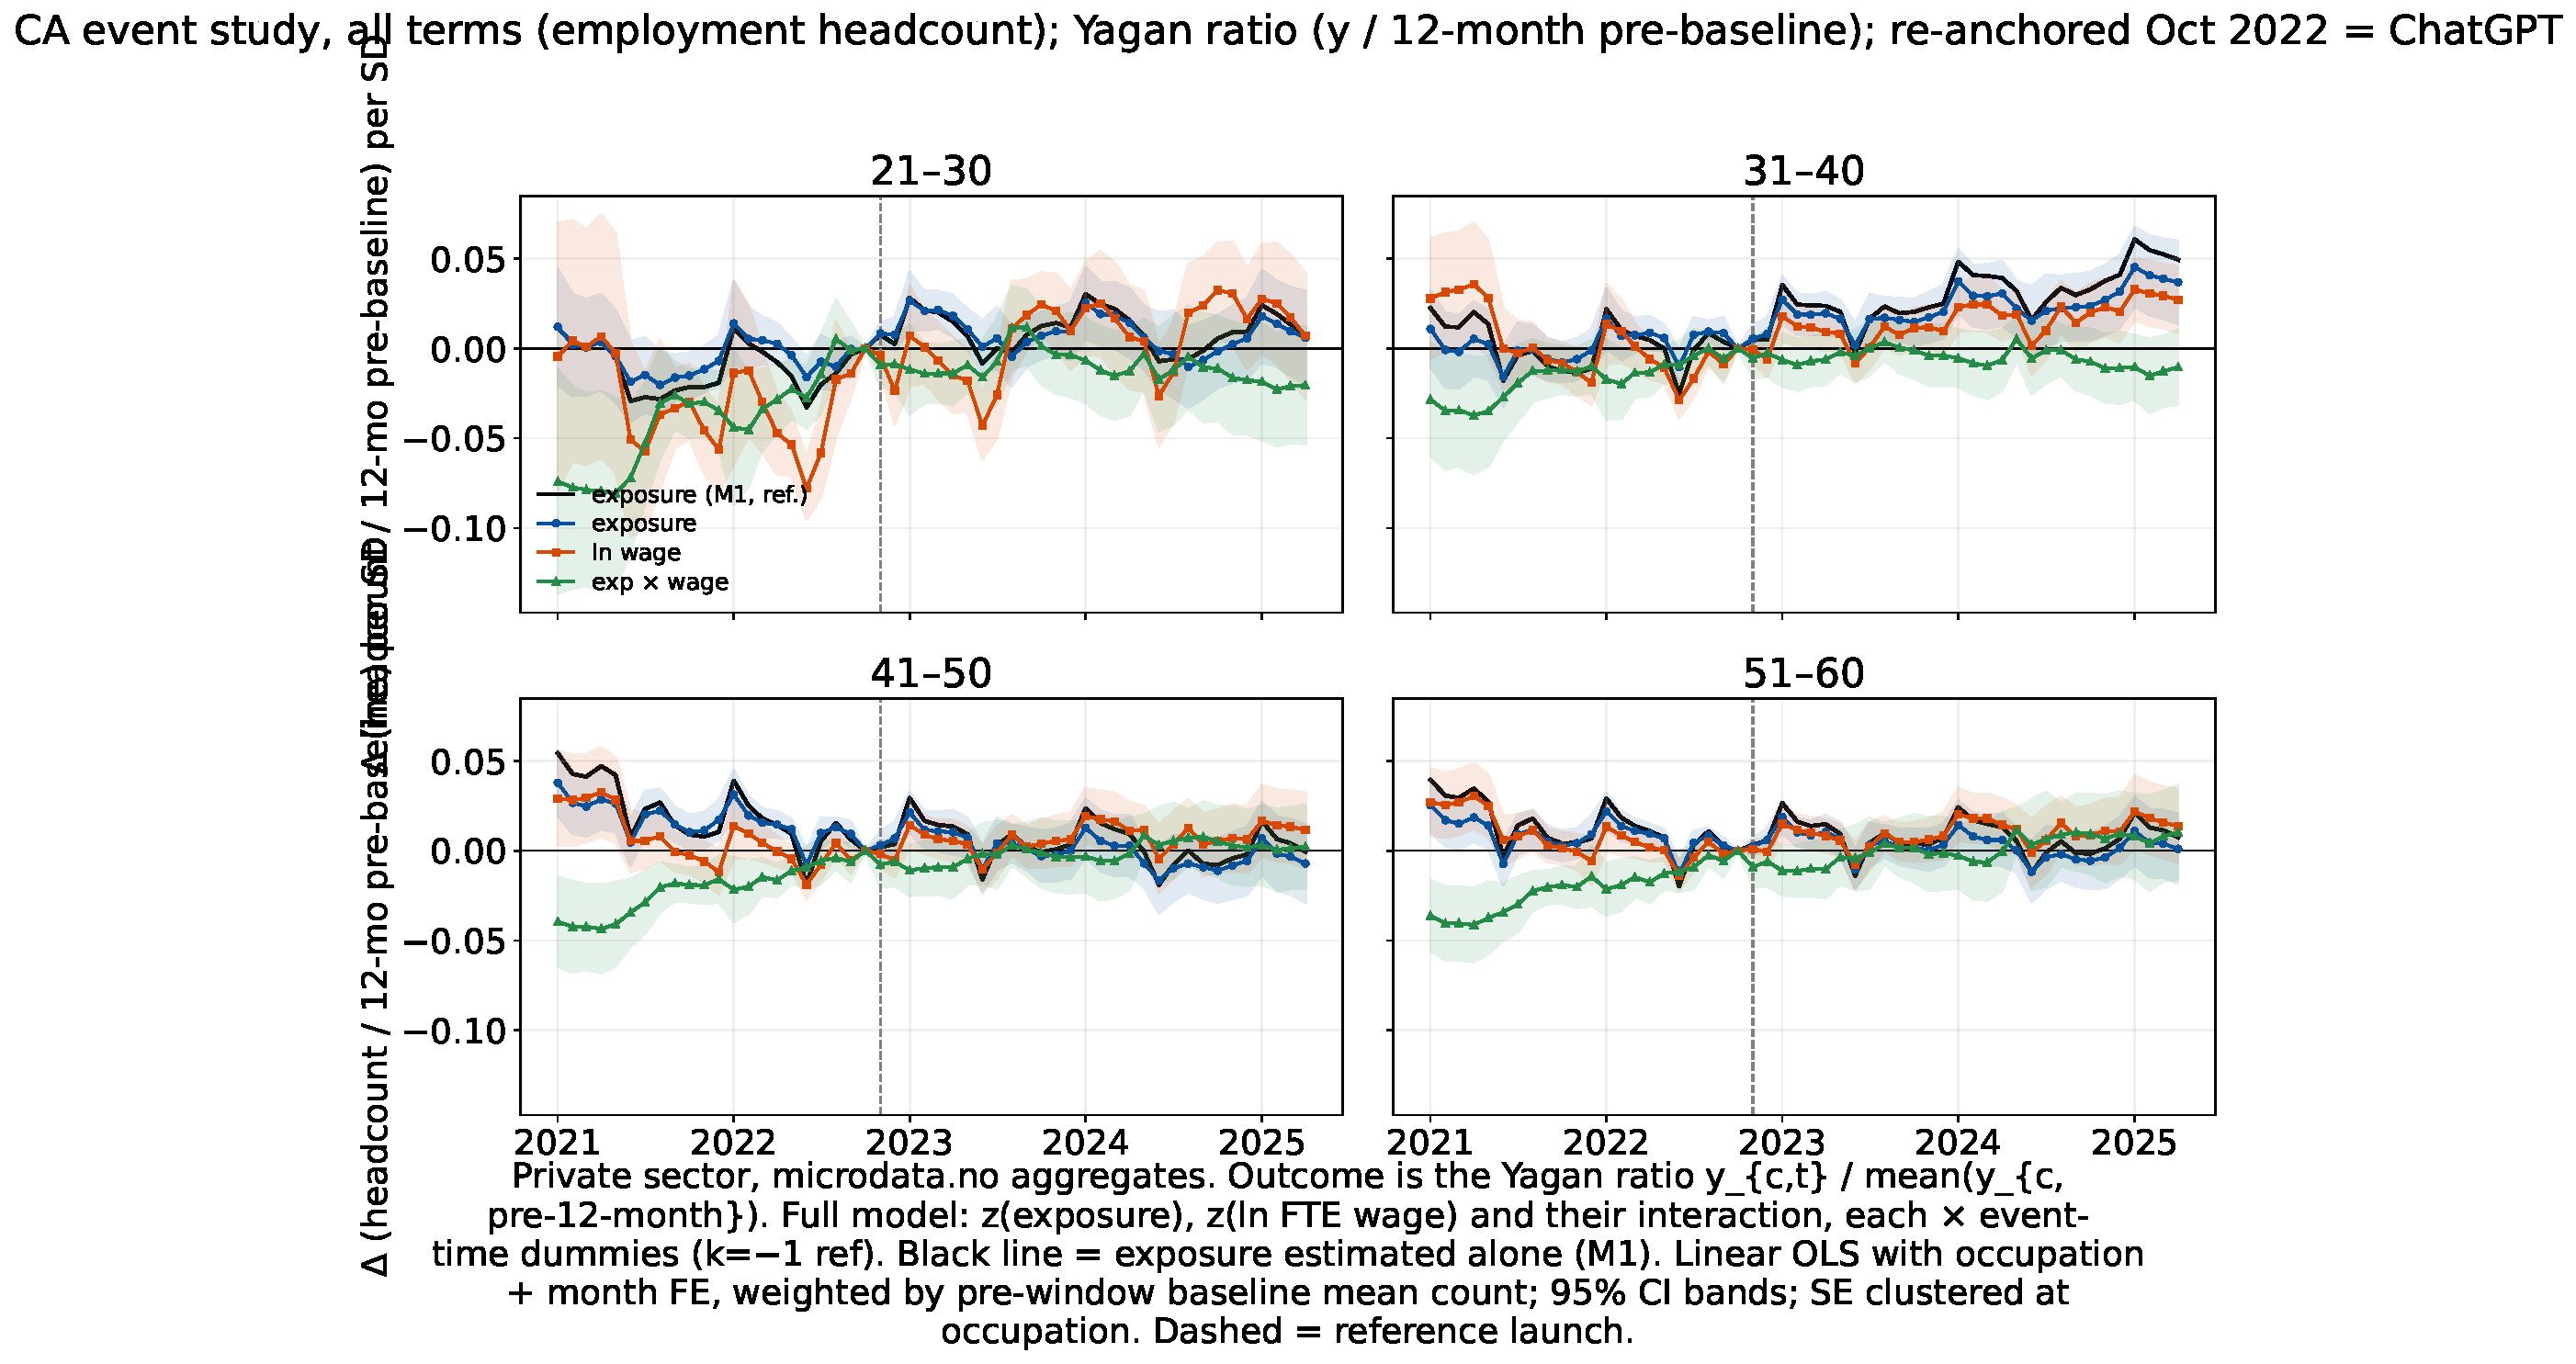
\includegraphics[width=\textwidth,height=0.42\textheight,keepaspectratio]{figure_ca_es_yagan_grid_count.pdf}\\[4pt]
  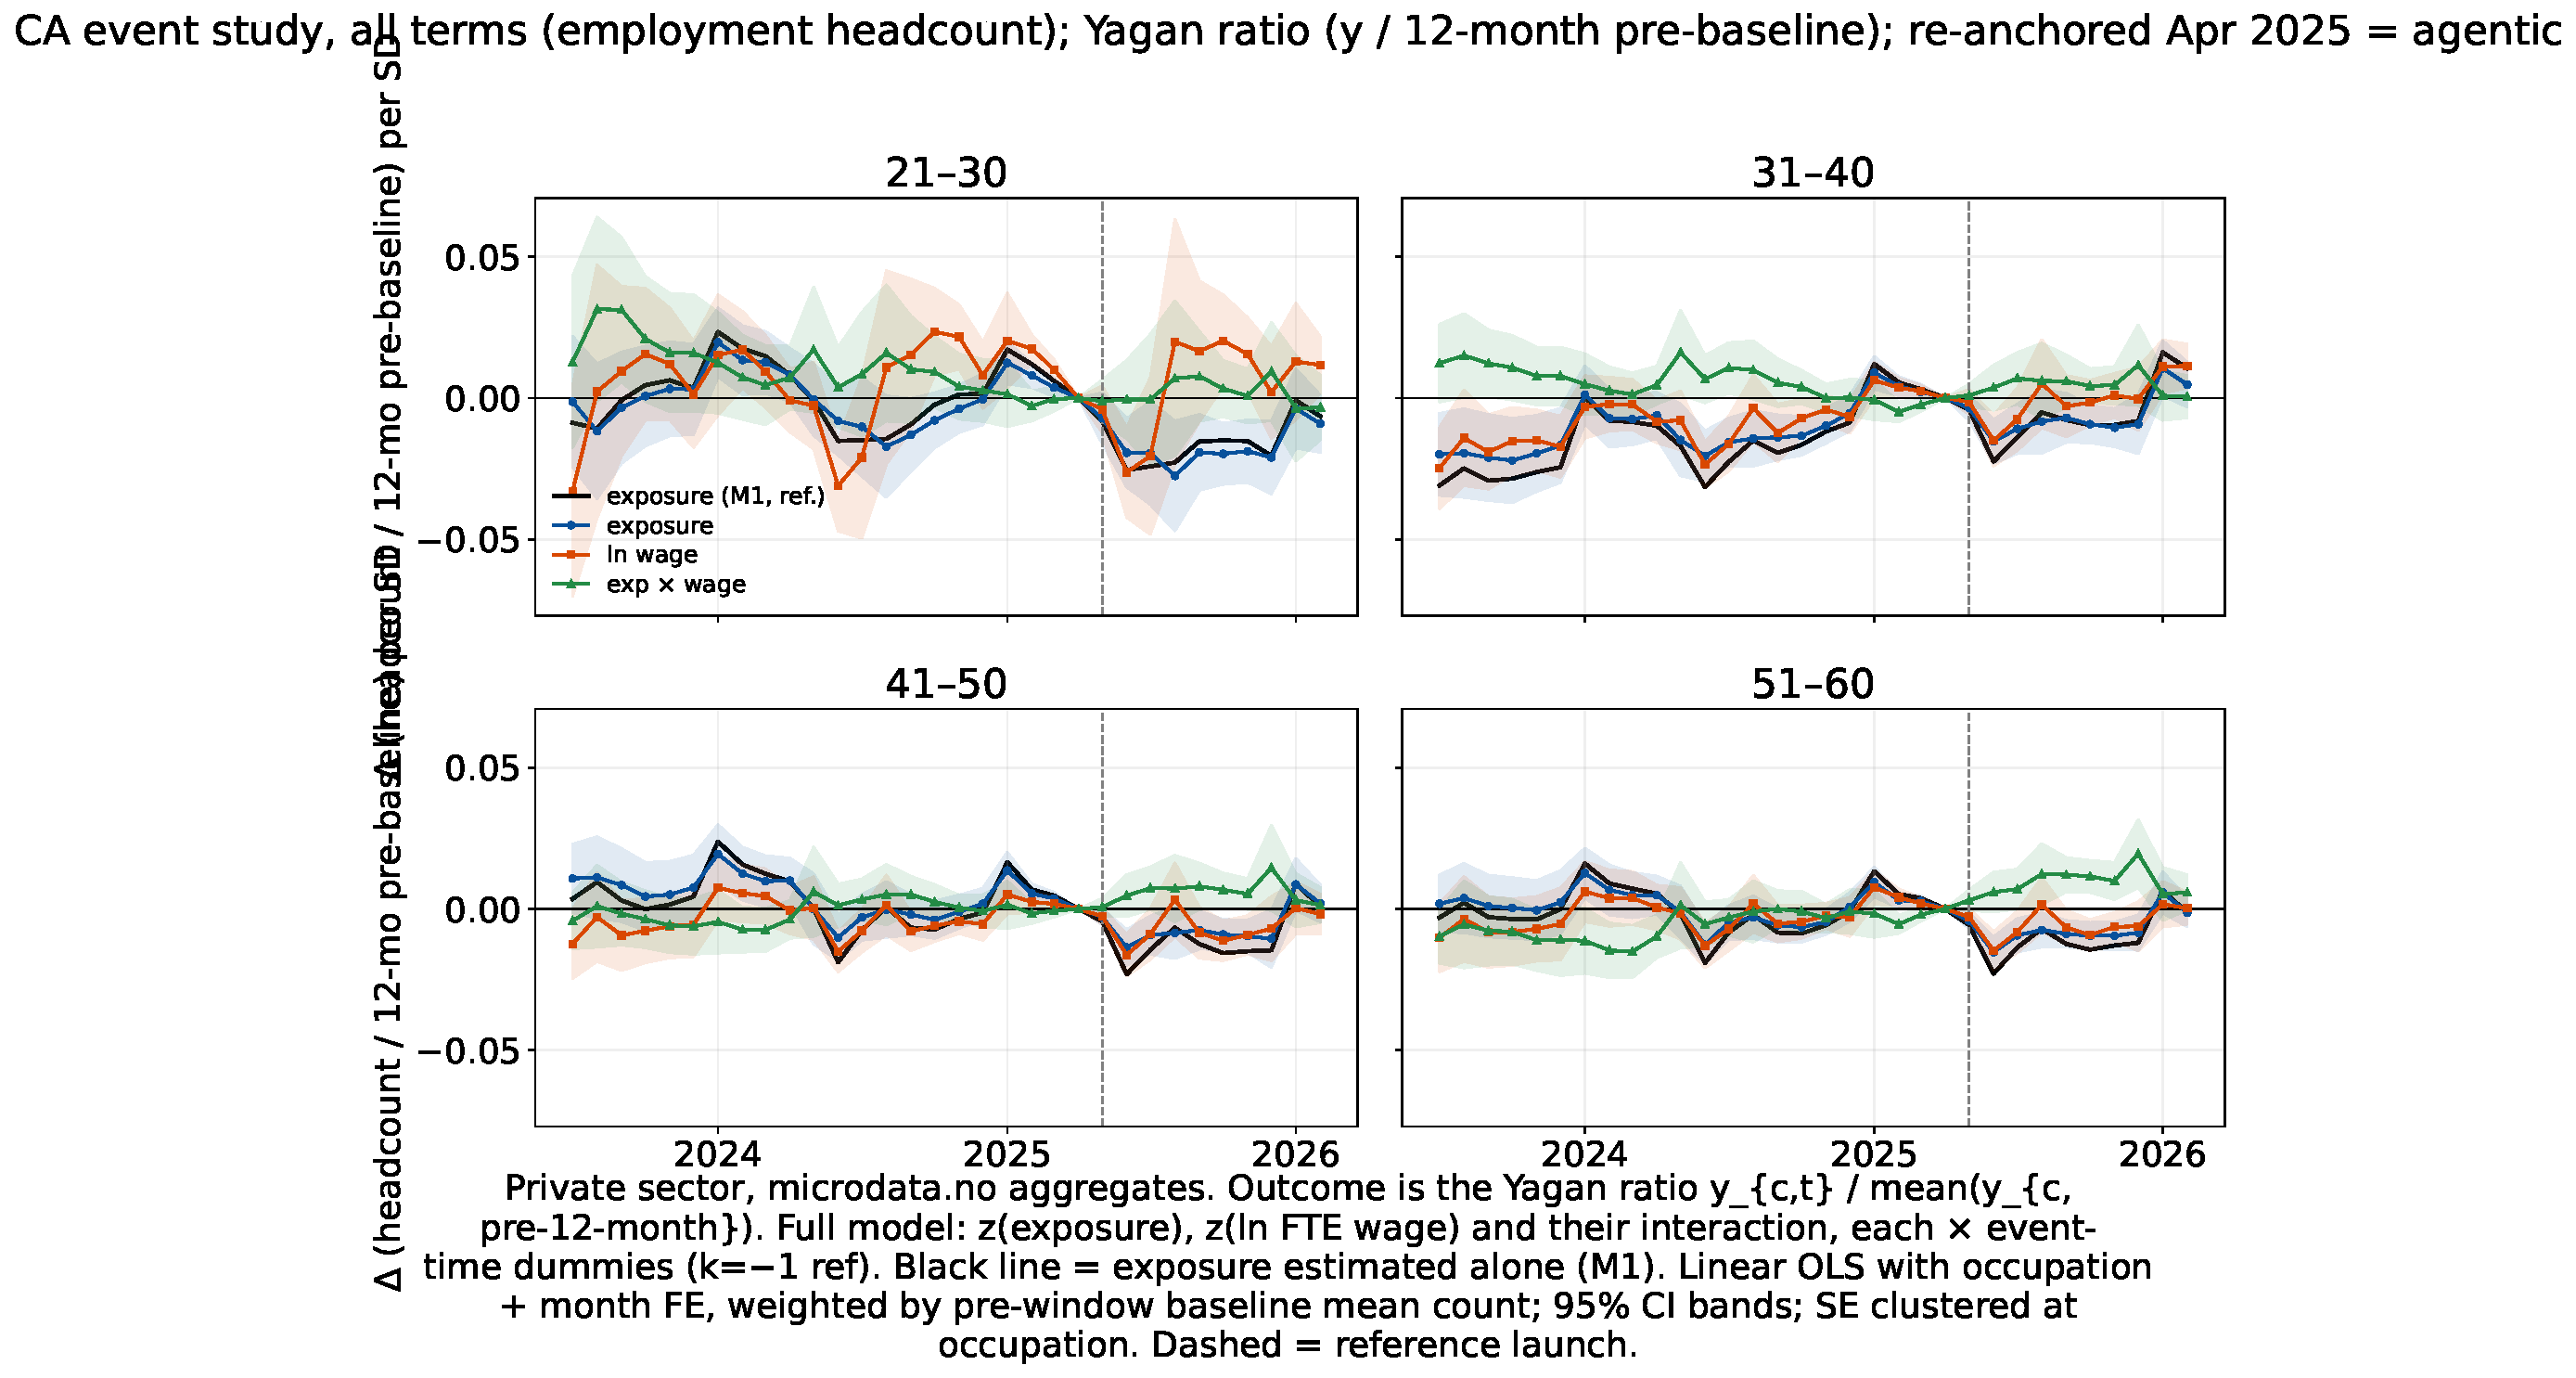
\includegraphics[width=\textwidth,height=0.42\textheight,keepaspectratio]{figure_ca_es_yagan_agentic_count.pdf}
  \caption{Yagan-ratio CA event study, employment headcount ---
           ChatGPT anchor (top), agentic anchor (bottom). Coefficients
           are $\Delta(y / \overline{y}_c^{\,\mathrm{pre}})$ per SD.}
\end{figure}

\clearpage
\subsection{New hires (nyjobb)}
\begin{figure}[H]\centering
  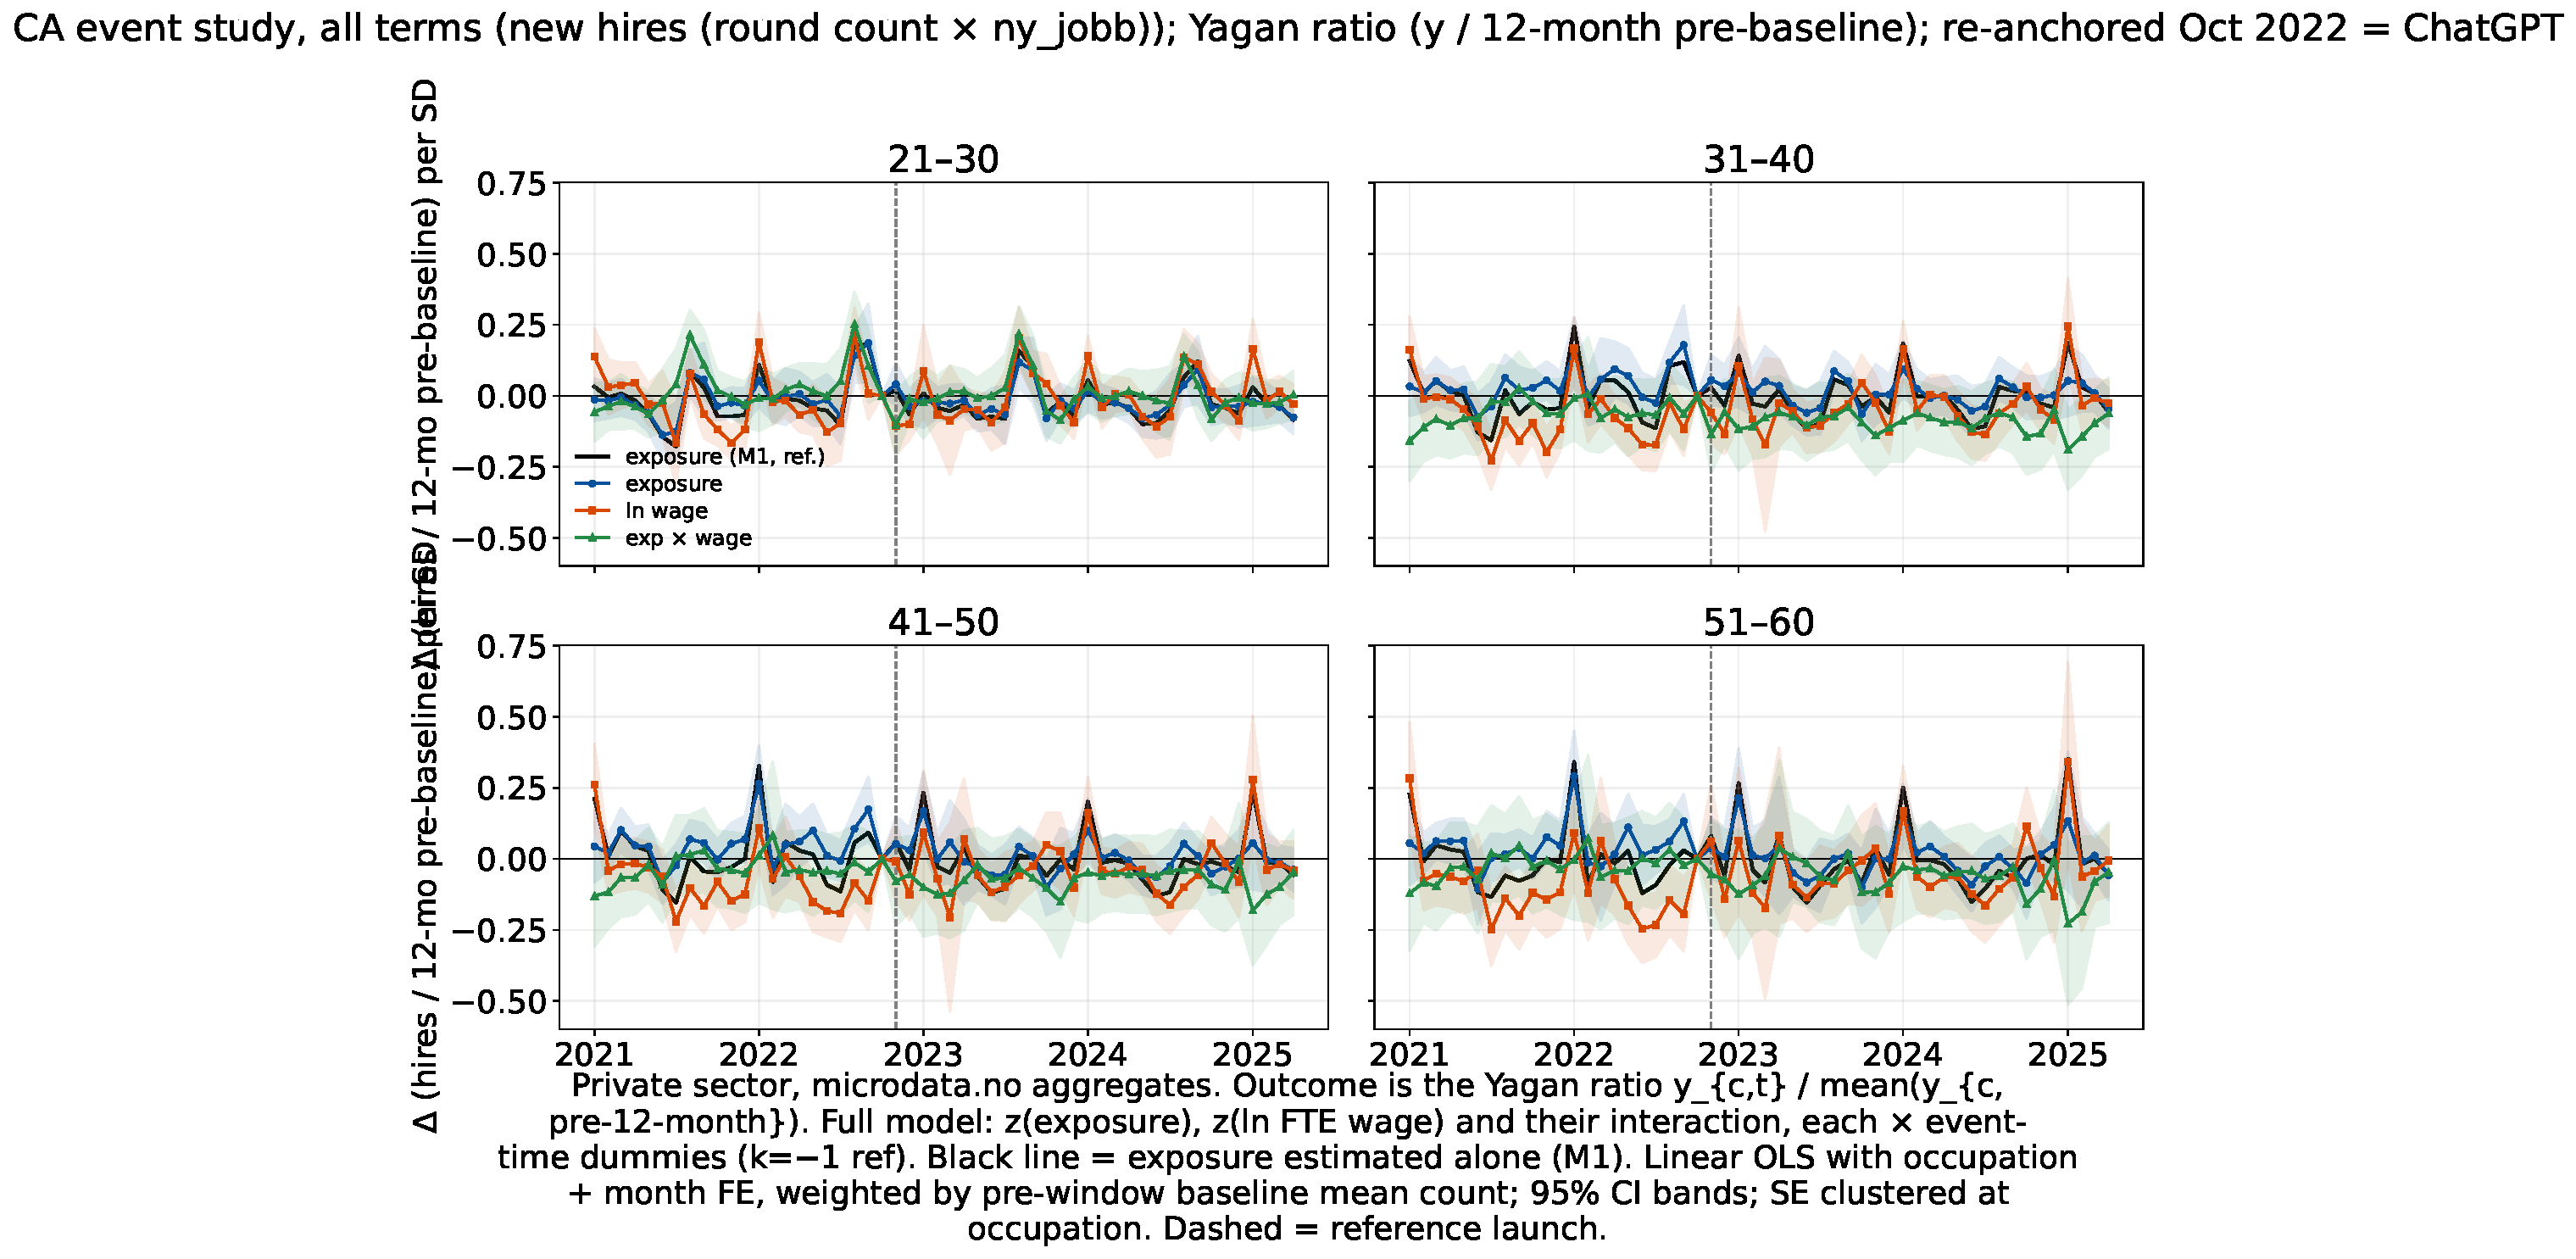
\includegraphics[width=\textwidth,height=0.42\textheight,keepaspectratio]{figure_ca_es_yagan_grid_nyjobb.pdf}\\[4pt]
  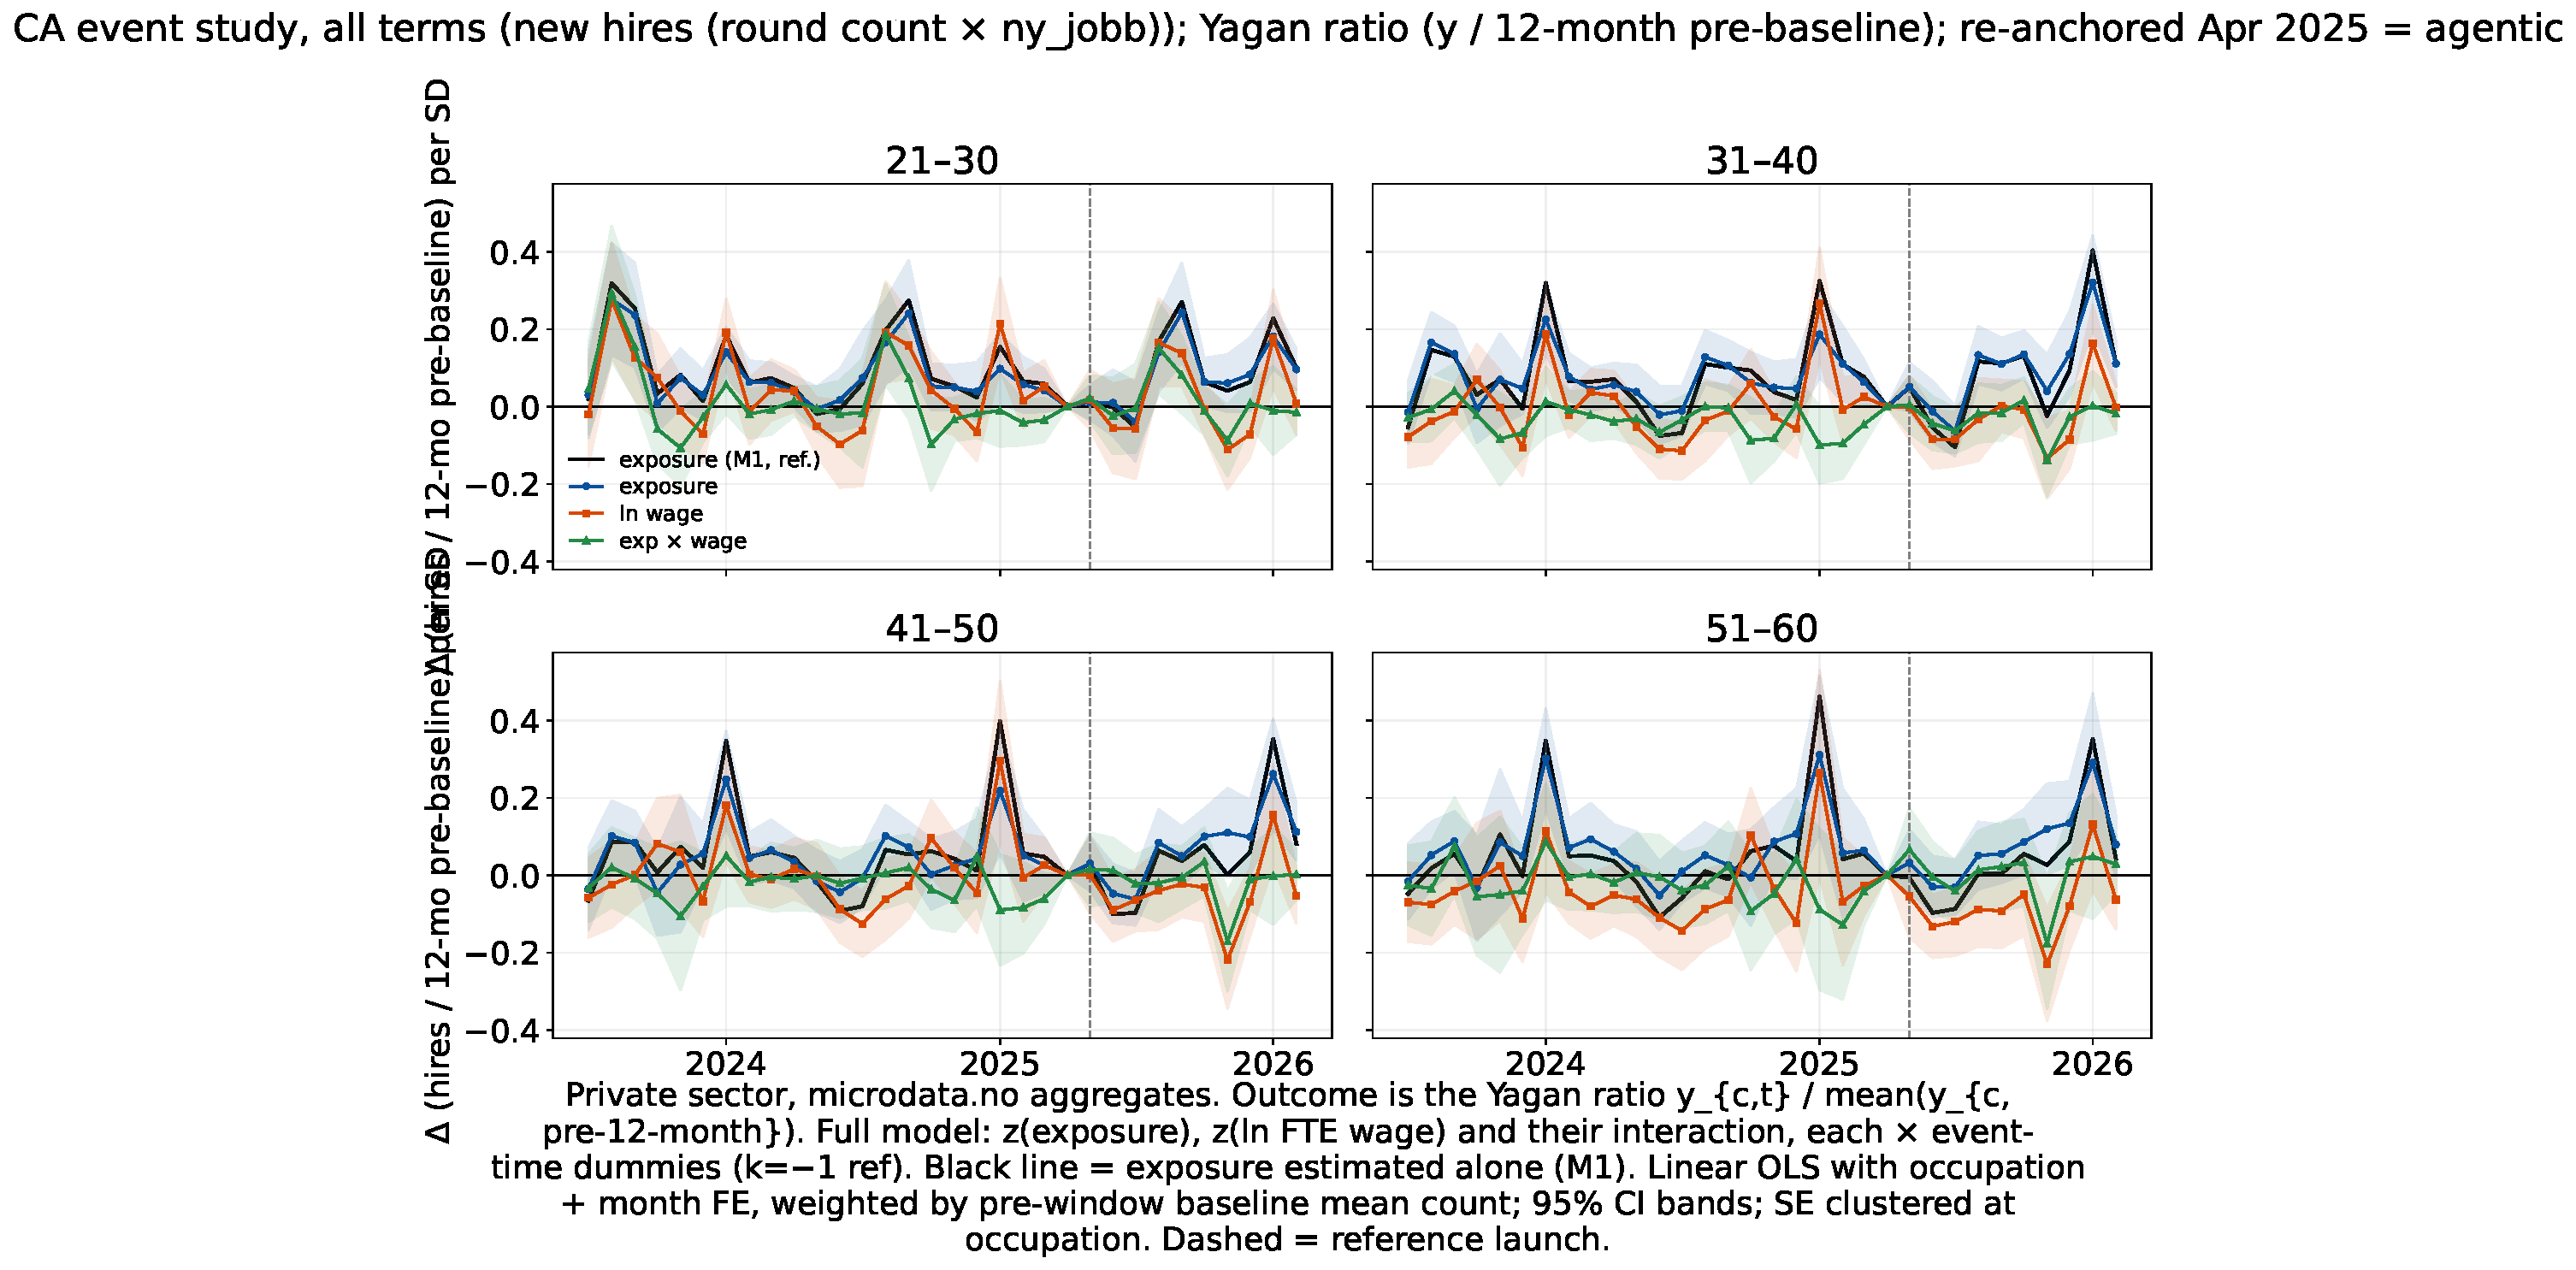
\includegraphics[width=\textwidth,height=0.42\textheight,keepaspectratio]{figure_ca_es_yagan_agentic_nyjobb.pdf}
  \caption{Yagan-ratio CA event study, new hires --- ChatGPT anchor
           (top), agentic anchor (bottom). Coefficients are
           $\Delta(y / \overline{y}_c^{\,\mathrm{pre}})$ per SD.}
\end{figure}

% =====================================================================
\clearpage
\section{Yagan-style pooled DiD (microdata.no, linear OLS)}

\noindent
Pooled-DiD counterpart to Section~7, mirroring Section~2's table format.
Each pre-period month enters as its own control level; all post months
collapse to ``POST'' with the reference month ($k=-1$) omitted, so each
POST coefficient is the average post-period effect on the Yagan ratio.
M1 = exposure only, M2 = ln wage only, M3 = both $+$ interaction.

\subsection{Employment (count)}
\begin{table}[H]\centering
\caption{Yagan-style CA pooled DiD on private-sector employment headcount (Yagan ratio ($y_{c,t} \,/\, \overline{y_c}_{,\mathrm{pre-12mo}}$)), by age group}
\label{tab:ca_did_yagan_combined_count}
\small
\begin{tabular}{lcccccc}
\toprule
 & \multicolumn{3}{c}{ChatGPT (ref.\ Oct 2022)} & \multicolumn{3}{c}{Agentic (ref.\ Apr 2025)} \\
\cmidrule(lr){2-4} \cmidrule(lr){5-7}
 & (1) & (2) & (3) & (4) & (5) & (6) \\
\midrule
\multicolumn{7}{@{}l}{\textit{Panel A: ages 21–30}} \\
Exposure $\times$ Post & +0.0101 &  & +0.0087 & -0.0154*** &  & -0.0165*** \\
 & (0.0070) &  & (0.0078) & (0.0053) &  & (0.0054) \\
ln wage $\times$ Post &  & +0.0110 & +0.0064 &  & -0.0005 & +0.0048 \\
 &  & (0.0086) & (0.0101) &  & (0.0083) & (0.0082) \\
Exp $\times$ wage $\times$ Post &  &  & -0.0103 &  &  & +0.0019 \\
 &  &  & (0.0104) &  &  & (0.0058) \\
\quad Observations & \multicolumn{3}{c}{20,124} & \multicolumn{3}{c}{12,320} \\
\quad Occupations & \multicolumn{3}{c}{387} & \multicolumn{3}{c}{385} \\
\midrule
\multicolumn{7}{@{}l}{\textit{Panel B: ages 31–40}} \\
Exposure $\times$ Post & +0.0299*** &  & +0.0231*** & -0.0054* &  & -0.0059* \\
 & (0.0062) &  & (0.0073) & (0.0031) &  & (0.0034) \\
ln wage $\times$ Post &  & +0.0263*** & +0.0146** &  & -0.0026 & -0.0000 \\
 &  & (0.0054) & (0.0057) &  & (0.0036) & (0.0039) \\
Exp $\times$ wage $\times$ Post &  &  & -0.0055 &  &  & +0.0045 \\
 &  &  & (0.0073) &  &  & (0.0035) \\
\quad Observations & \multicolumn{3}{c}{19,968} & \multicolumn{3}{c}{12,288} \\
\quad Occupations & \multicolumn{3}{c}{384} & \multicolumn{3}{c}{384} \\
\midrule
\multicolumn{7}{@{}l}{\textit{Panel C: ages 41–50}} \\
Exposure $\times$ Post & +0.0043 &  & +0.0003 & -0.0096*** &  & -0.0060** \\
 & (0.0061) &  & (0.0072) & (0.0023) &  & (0.0026) \\
ln wage $\times$ Post &  & +0.0071 & +0.0071 &  & -0.0090*** & -0.0062* \\
 &  & (0.0058) & (0.0067) &  & (0.0029) & (0.0033) \\
Exp $\times$ wage $\times$ Post &  &  & -0.0011 &  &  & +0.0059** \\
 &  &  & (0.0087) &  &  & (0.0030) \\
\quad Observations & \multicolumn{3}{c}{20,020} & \multicolumn{3}{c}{12,256} \\
\quad Occupations & \multicolumn{3}{c}{385} & \multicolumn{3}{c}{383} \\
\midrule
\multicolumn{7}{@{}l}{\textit{Panel D: ages 51–60}} \\
Exposure $\times$ Post & +0.0078 &  & +0.0031 & -0.0096*** &  & -0.0068*** \\
 & (0.0056) &  & (0.0061) & (0.0019) &  & (0.0019) \\
ln wage $\times$ Post &  & +0.0113** & +0.0096 &  & -0.0074*** & -0.0051** \\
 &  & (0.0055) & (0.0062) &  & (0.0022) & (0.0023) \\
Exp $\times$ wage $\times$ Post &  &  & +0.0006 &  &  & +0.0093*** \\
 &  &  & (0.0092) &  &  & (0.0024) \\
\quad Observations & \multicolumn{3}{c}{20,176} & \multicolumn{3}{c}{12,288} \\
\quad Occupations & \multicolumn{3}{c}{388} & \multicolumn{3}{c}{384} \\
\midrule
Occupation FE & Yes & Yes & Yes & Yes & Yes & Yes \\
Month FE & Yes & Yes & Yes & Yes & Yes & Yes \\
\bottomrule
\end{tabular}
\begin{minipage}{\linewidth}\vspace{2pt}\footnotesize
\emph{Notes:} Linear OLS (\texttt{fixest::feols}) on the microdata.no cell aggregates (private sector, sektor = 2). Outcome is the Yagan ratio $y_{c,t} / \overline{y_c}_{,\mathrm{pre}}$ where the baseline is the mean of $y$ over the 12-month pre-window $k \in [-12, -1]$. Columns (1)--(3): ChatGPT window (Oct 2022 $=k{=}{-}1$, through 2025m4); (4)--(6): agentic (Apr 2025 $=k{=}{-}1$, from 2023m7). Each coefficient is the average post-period effect relative to the reference month ($k{=}{-}1$); each pre-period month enters as a separate control. M1 = exposure only, M2 = ln wage only, M3 = both $+$ interaction. Treatments standardized: $z(\text{exp})$ = Eloundou $\beta$ (pooled), $z(\text{lnw})$ = ln full-time-equivalent wage (pre-ChatGPT, within age group). Cells weighted by the pre-window baseline mean count. Occupation $+$ month FE; SE clustered at occupation in parentheses. $^{*}p<0.10$, $^{**}p<0.05$, $^{***}p<0.01$.
\end{minipage}
\end{table}

\clearpage
\subsection{New hires (nyjobb)}
\begin{table}[H]\centering
\caption{Yagan-style CA pooled DiD on private-sector new hires = round(count $\times$ ny\_jobb) (Yagan ratio ($y_{c,t} \,/\, \overline{y_c}_{,\mathrm{pre-12mo}}$)), by age group}
\label{tab:ca_did_yagan_combined_nyjobb}
\small
\begin{tabular}{lcccccc}
\toprule
 & \multicolumn{3}{c}{ChatGPT (ref.\ Oct 2022)} & \multicolumn{3}{c}{Agentic (ref.\ Apr 2025)} \\
\cmidrule(lr){2-4} \cmidrule(lr){5-7}
 & (1) & (2) & (3) & (4) & (5) & (6) \\
\midrule
\multicolumn{7}{@{}l}{\textit{Panel A: ages 21–30}} \\
Exposure $\times$ Post & -0.0213 &  & -0.0195 & +0.0894*** &  & +0.0853*** \\
 & (0.0233) &  & (0.0256) & (0.0237) &  & (0.0257) \\
ln wage $\times$ Post &  & -0.0131 & -0.0055 &  & +0.0450 & +0.0205 \\
 &  & (0.0219) & (0.0251) &  & (0.0305) & (0.0302) \\
Exp $\times$ wage $\times$ Post &  &  & +0.0022 &  &  & +0.0113 \\
 &  &  & (0.0343) &  &  & (0.0234) \\
\quad Observations & \multicolumn{3}{c}{18,668} & \multicolumn{3}{c}{11,392} \\
\quad Occupations & \multicolumn{3}{c}{359} & \multicolumn{3}{c}{356} \\
\midrule
\multicolumn{7}{@{}l}{\textit{Panel B: ages 31–40}} \\
Exposure $\times$ Post & -0.0036 &  & +0.0123 & +0.0833*** &  & +0.0962*** \\
 & (0.0350) &  & (0.0307) & (0.0224) &  & (0.0251) \\
ln wage $\times$ Post &  & -0.0288 & -0.0354 &  & +0.0207 & -0.0265 \\
 &  & (0.0366) & (0.0345) &  & (0.0249) & (0.0255) \\
Exp $\times$ wage $\times$ Post &  &  & -0.0937 &  &  & -0.0296 \\
 &  &  & (0.0573) &  &  & (0.0211) \\
\quad Observations & \multicolumn{3}{c}{18,980} & \multicolumn{3}{c}{11,392} \\
\quad Occupations & \multicolumn{3}{c}{365} & \multicolumn{3}{c}{356} \\
\midrule
\multicolumn{7}{@{}l}{\textit{Panel C: ages 41–50}} \\
Exposure $\times$ Post & -0.0085 &  & +0.0017 & +0.0504** &  & +0.0737** \\
 & (0.0359) &  & (0.0267) & (0.0196) &  & (0.0301) \\
ln wage $\times$ Post &  & -0.0300 & -0.0310 &  & -0.0035 & -0.0432 \\
 &  & (0.0394) & (0.0409) &  & (0.0268) & (0.0344) \\
Exp $\times$ wage $\times$ Post &  &  & -0.0746 &  &  & -0.0166 \\
 &  &  & (0.0664) &  &  & (0.0308) \\
\quad Observations & \multicolumn{3}{c}{18,772} & \multicolumn{3}{c}{11,488} \\
\quad Occupations & \multicolumn{3}{c}{361} & \multicolumn{3}{c}{359} \\
\midrule
\multicolumn{7}{@{}l}{\textit{Panel D: ages 51–60}} \\
Exposure $\times$ Post & -0.0060 &  & +0.0051 & +0.0380 &  & +0.0789** \\
 & (0.0376) &  & (0.0296) & (0.0253) &  & (0.0346) \\
ln wage $\times$ Post &  & -0.0372 & -0.0387 &  & -0.0401 & -0.0779* \\
 &  & (0.0483) & (0.0545) &  & (0.0349) & (0.0406) \\
Exp $\times$ wage $\times$ Post &  &  & -0.0678 &  &  & +0.0025 \\
 &  &  & (0.0764) &  &  & (0.0409) \\
\quad Observations & \multicolumn{3}{c}{18,564} & \multicolumn{3}{c}{11,104} \\
\quad Occupations & \multicolumn{3}{c}{357} & \multicolumn{3}{c}{347} \\
\midrule
Occupation FE & Yes & Yes & Yes & Yes & Yes & Yes \\
Month FE & Yes & Yes & Yes & Yes & Yes & Yes \\
\bottomrule
\end{tabular}
\begin{minipage}{\linewidth}\vspace{2pt}\footnotesize
\emph{Notes:} Linear OLS (\texttt{fixest::feols}) on the microdata.no cell aggregates (private sector, sektor = 2). Outcome is the Yagan ratio $y_{c,t} / \overline{y_c}_{,\mathrm{pre}}$ where the baseline is the mean of $y$ over the 12-month pre-window $k \in [-12, -1]$. Columns (1)--(3): ChatGPT window (Oct 2022 $=k{=}{-}1$, through 2025m4); (4)--(6): agentic (Apr 2025 $=k{=}{-}1$, from 2023m7). Each coefficient is the average post-period effect relative to the reference month ($k{=}{-}1$); each pre-period month enters as a separate control. M1 = exposure only, M2 = ln wage only, M3 = both $+$ interaction. Treatments standardized: $z(\text{exp})$ = Eloundou $\beta$ (pooled), $z(\text{lnw})$ = ln full-time-equivalent wage (pre-ChatGPT, within age group). Cells weighted by the pre-window baseline mean count. Occupation $+$ month FE; SE clustered at occupation in parentheses. $^{*}p<0.10$, $^{**}p<0.05$, $^{***}p<0.01$.
\end{minipage}
\end{table}

% =====================================================================
\clearpage
\section{Robustness: YoY-matched event studies (microdata.no, linear OLS)}

\noindent
Sections~7--8 used the \emph{mean} of $y$ over the 12-month pre-window as
the baseline for each cell. This chapter is a robustness check that
replaces that pooled-mean baseline with a \emph{same-month-of-year}
match inside the same 12-month pre-window. Concretely, for each
cell $c$ and post-period month $t$, the baseline is the unique
pre-window observation $y_{c, m(t)}$ where $m(t)$ has the same
month-of-year as $t$:
\begin{equation*}
  y^{\mathrm{YoY}}_{c,t}=\frac{y_{c,t}}{y_{c, m(t)}},
\end{equation*}
with $m(t)\in\{$2021m11, $\ldots,$ 2022m10$\}$ for ChatGPT and
$\{$2024m05, $\ldots,$ 2025m04$\}$ for agentic.
\medskip

\noindent
This strips out seasonality (sysselsetting, hires and wages all have
strong calendar-month patterns) without leaving the pre-treatment
window: the baseline is \emph{anchored} at the 12-month pre-window and
reused each year, so it never gets contaminated by post-treatment
observations even at $k \geq 12$. By construction $y^{\mathrm{YoY}} = 1$
for every $k \in [-12,-1]$ (numerator and denominator are the same
observation), so pre-period event-time coefficients inside the
baseline window are mechanically zero --- there is no cross-occupation
variation in the LHS to identify off. Pre-trend tests therefore have
to use $k < -12$, where the baseline lies twelve months ahead of the
data month. Cells with baseline $y = 0$ are dropped (ratio undefined;
feols rejects zero weights). Estimator, FE structure, weights and
cluster are identical to Section~7 (linear OLS, occupation $+$ month
FE, cells weighted by the pre-window baseline count, SE clustered at
occupation); only the construction of the ratio's denominator differs.

\subsection{Employment (count)}
\begin{figure}[H]\centering
  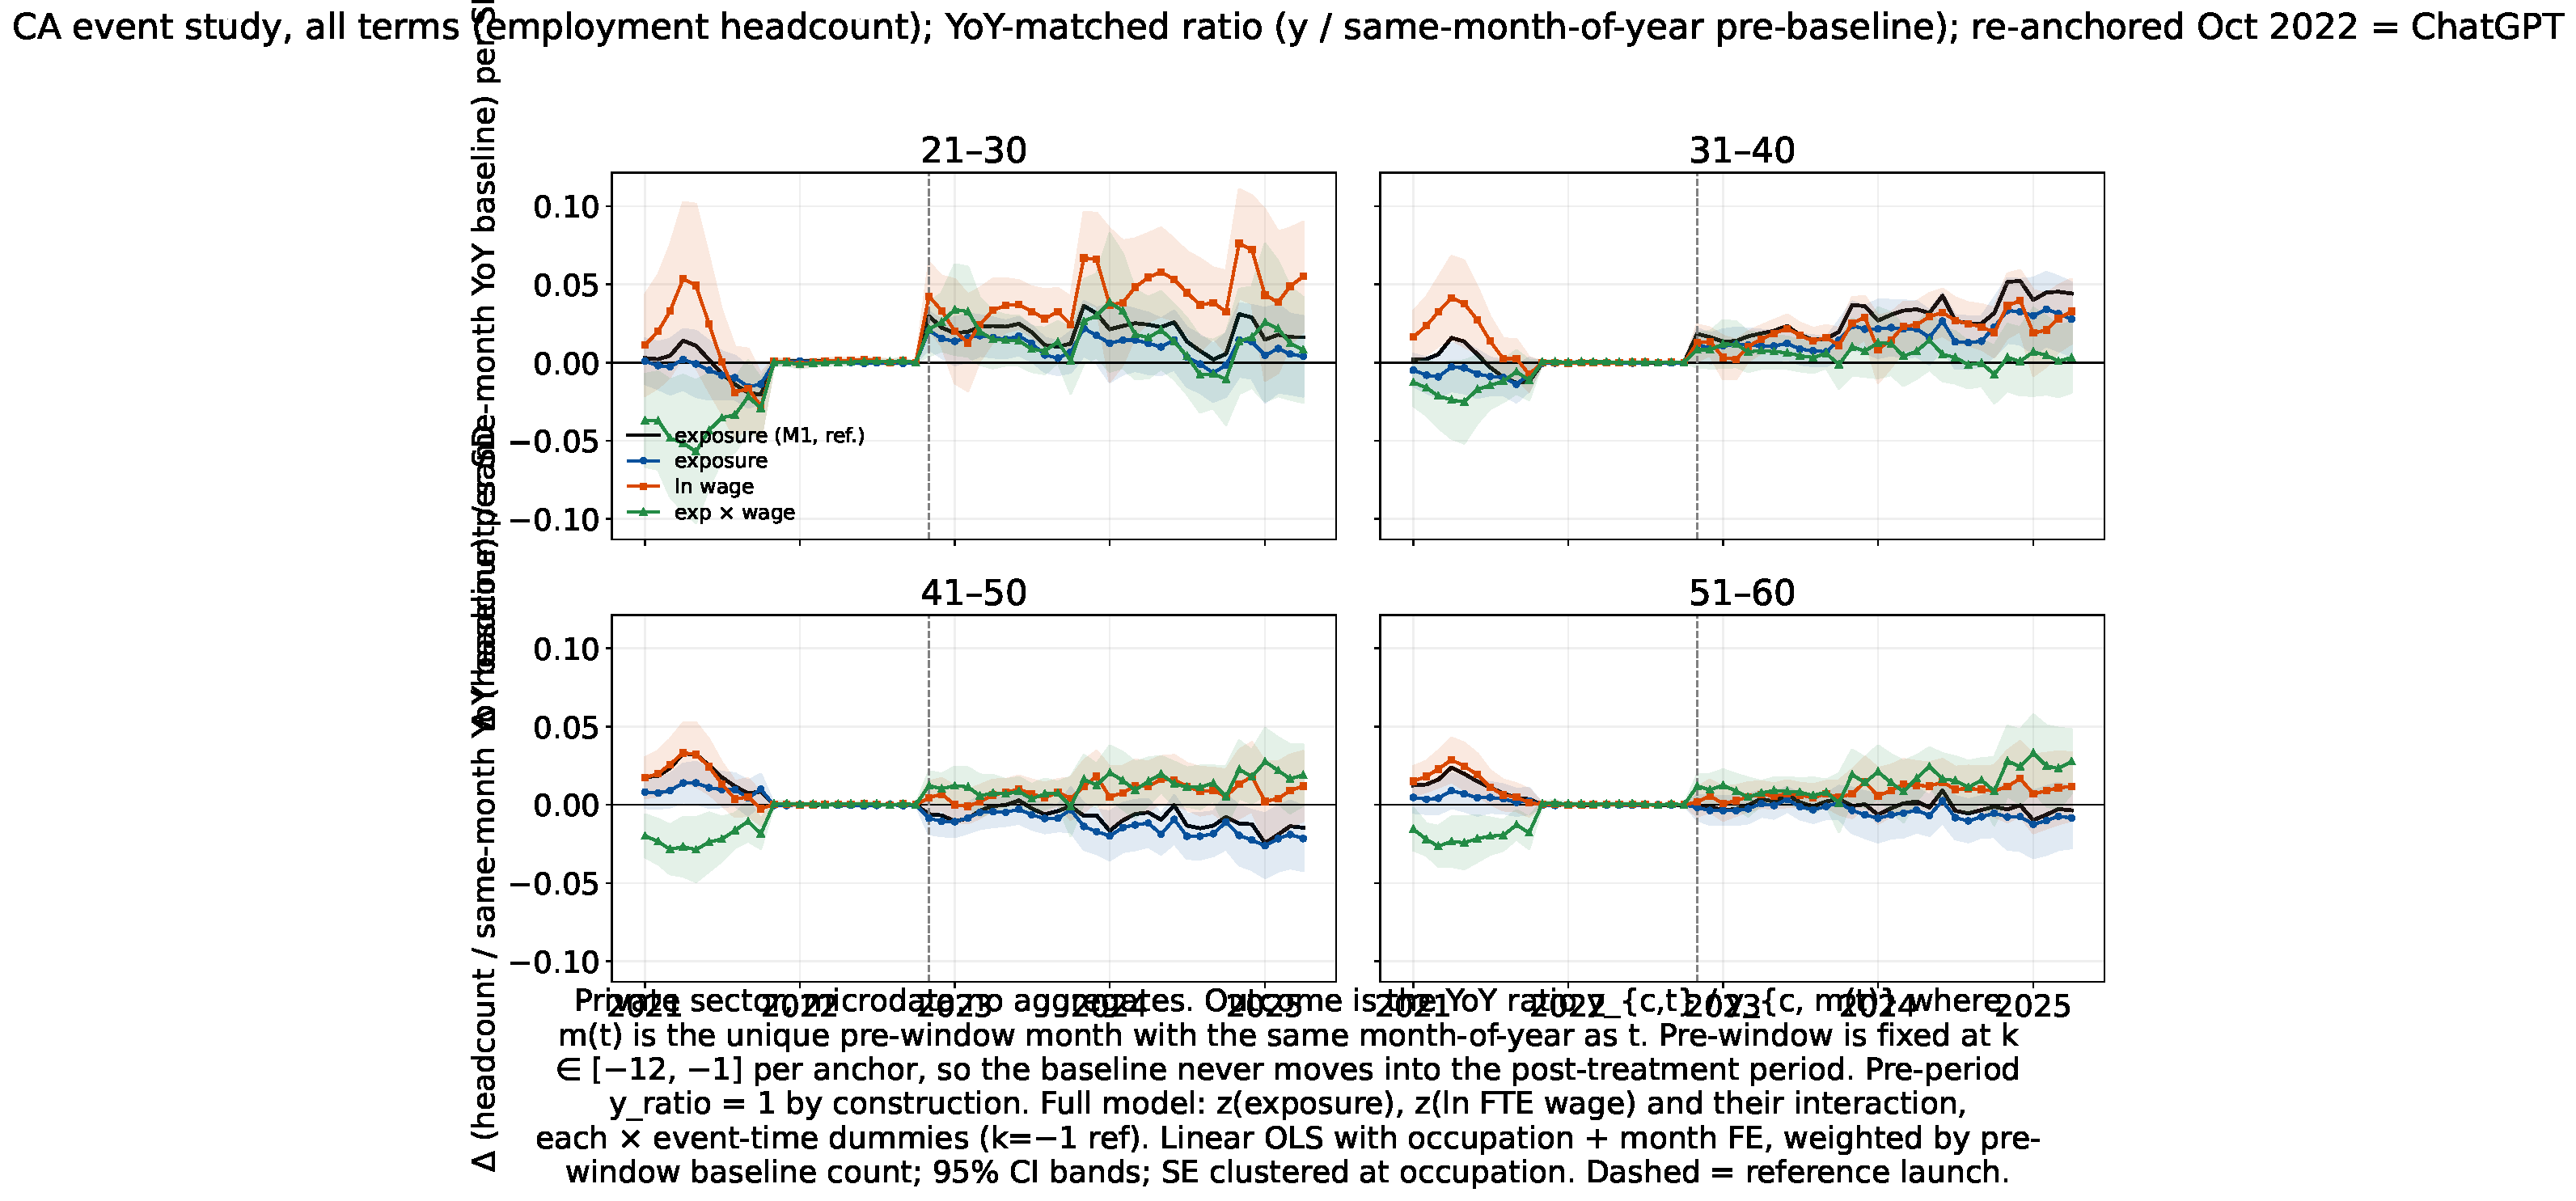
\includegraphics[width=\textwidth,height=0.42\textheight,keepaspectratio]{figure_ca_es_yoy_grid_count.pdf}\\[4pt]
  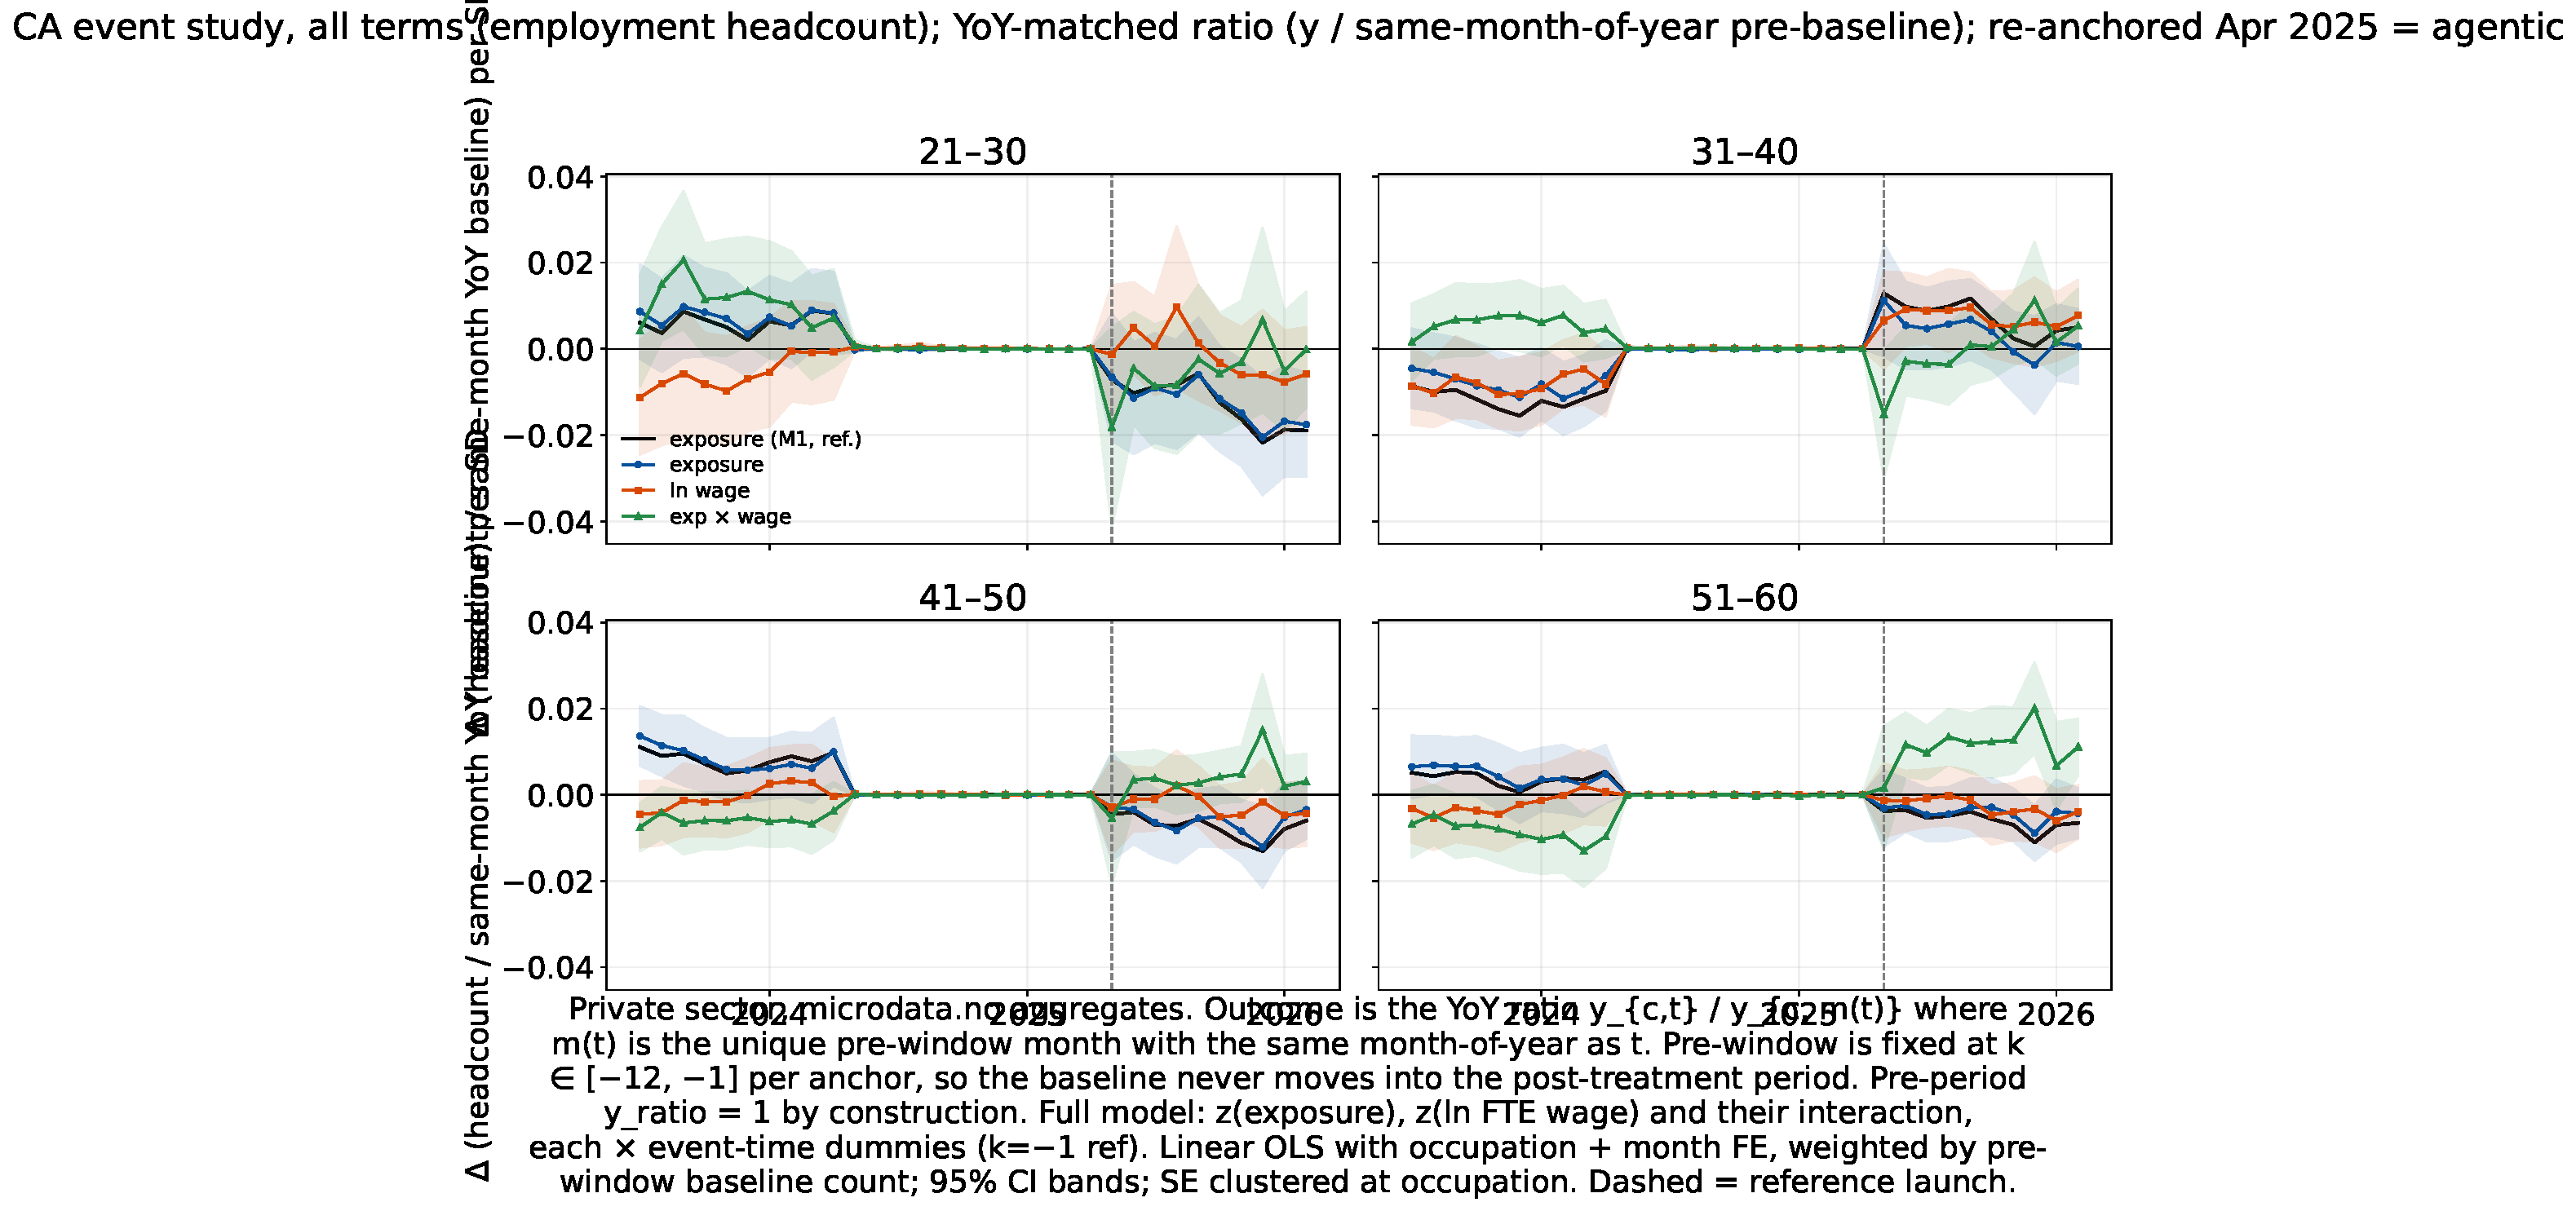
\includegraphics[width=\textwidth,height=0.42\textheight,keepaspectratio]{figure_ca_es_yoy_agentic_count.pdf}
  \caption{YoY-matched CA event study, employment headcount ---
           ChatGPT anchor (top), agentic anchor (bottom). Coefficients
           are $\Delta(y_{c,t}/y_{c, m(t)})$ per SD.}
\end{figure}

\clearpage
\subsection{New hires (nyjobb)}
\begin{figure}[H]\centering
  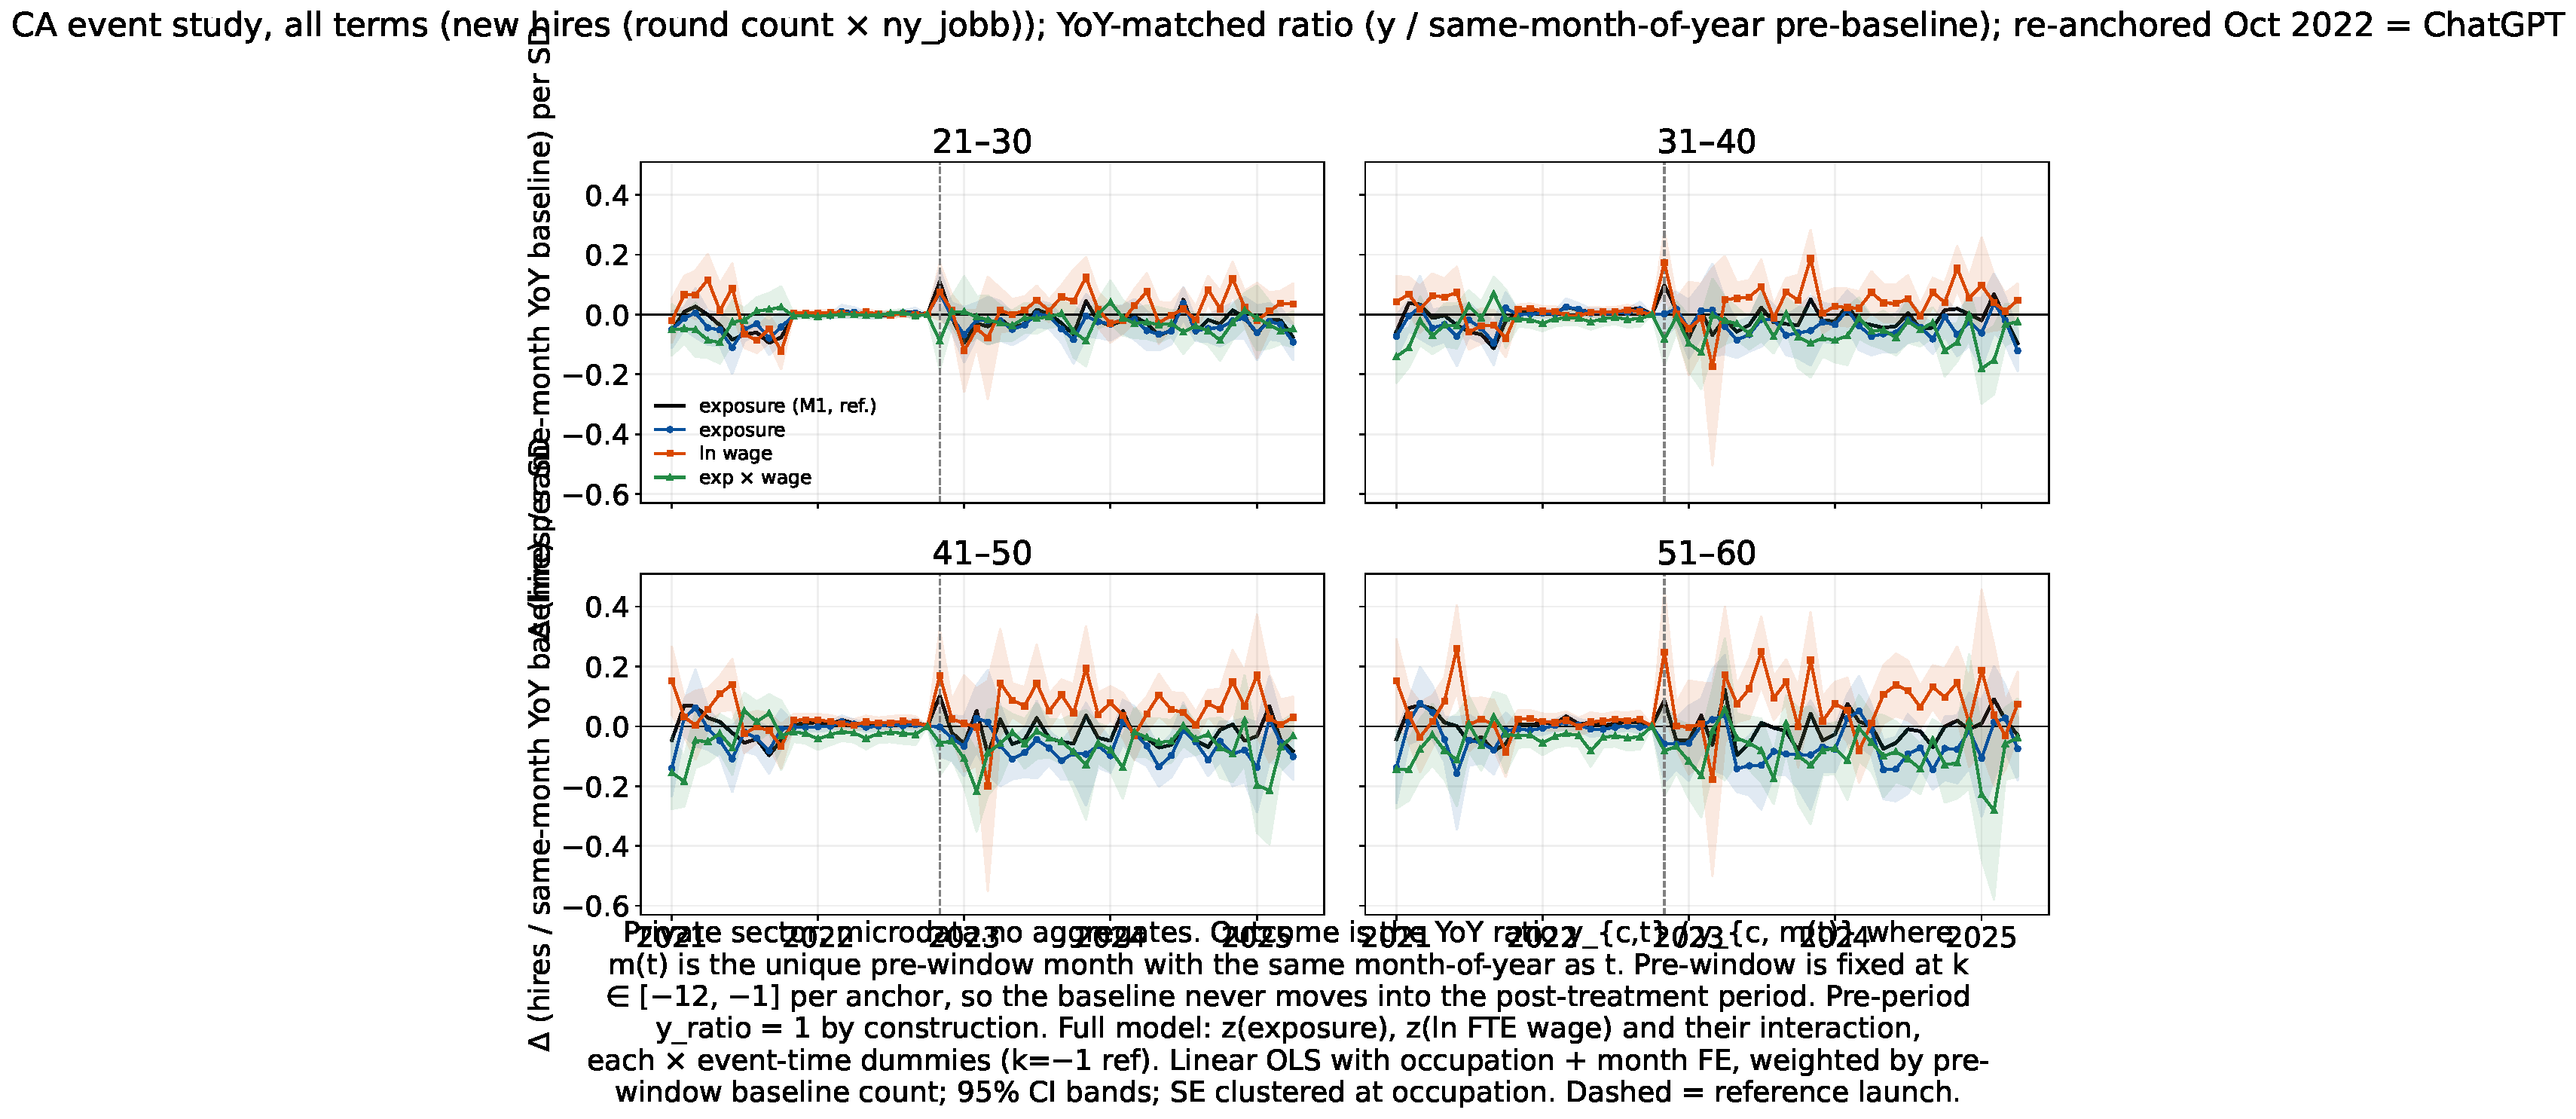
\includegraphics[width=\textwidth,height=0.42\textheight,keepaspectratio]{figure_ca_es_yoy_grid_nyjobb.pdf}\\[4pt]
  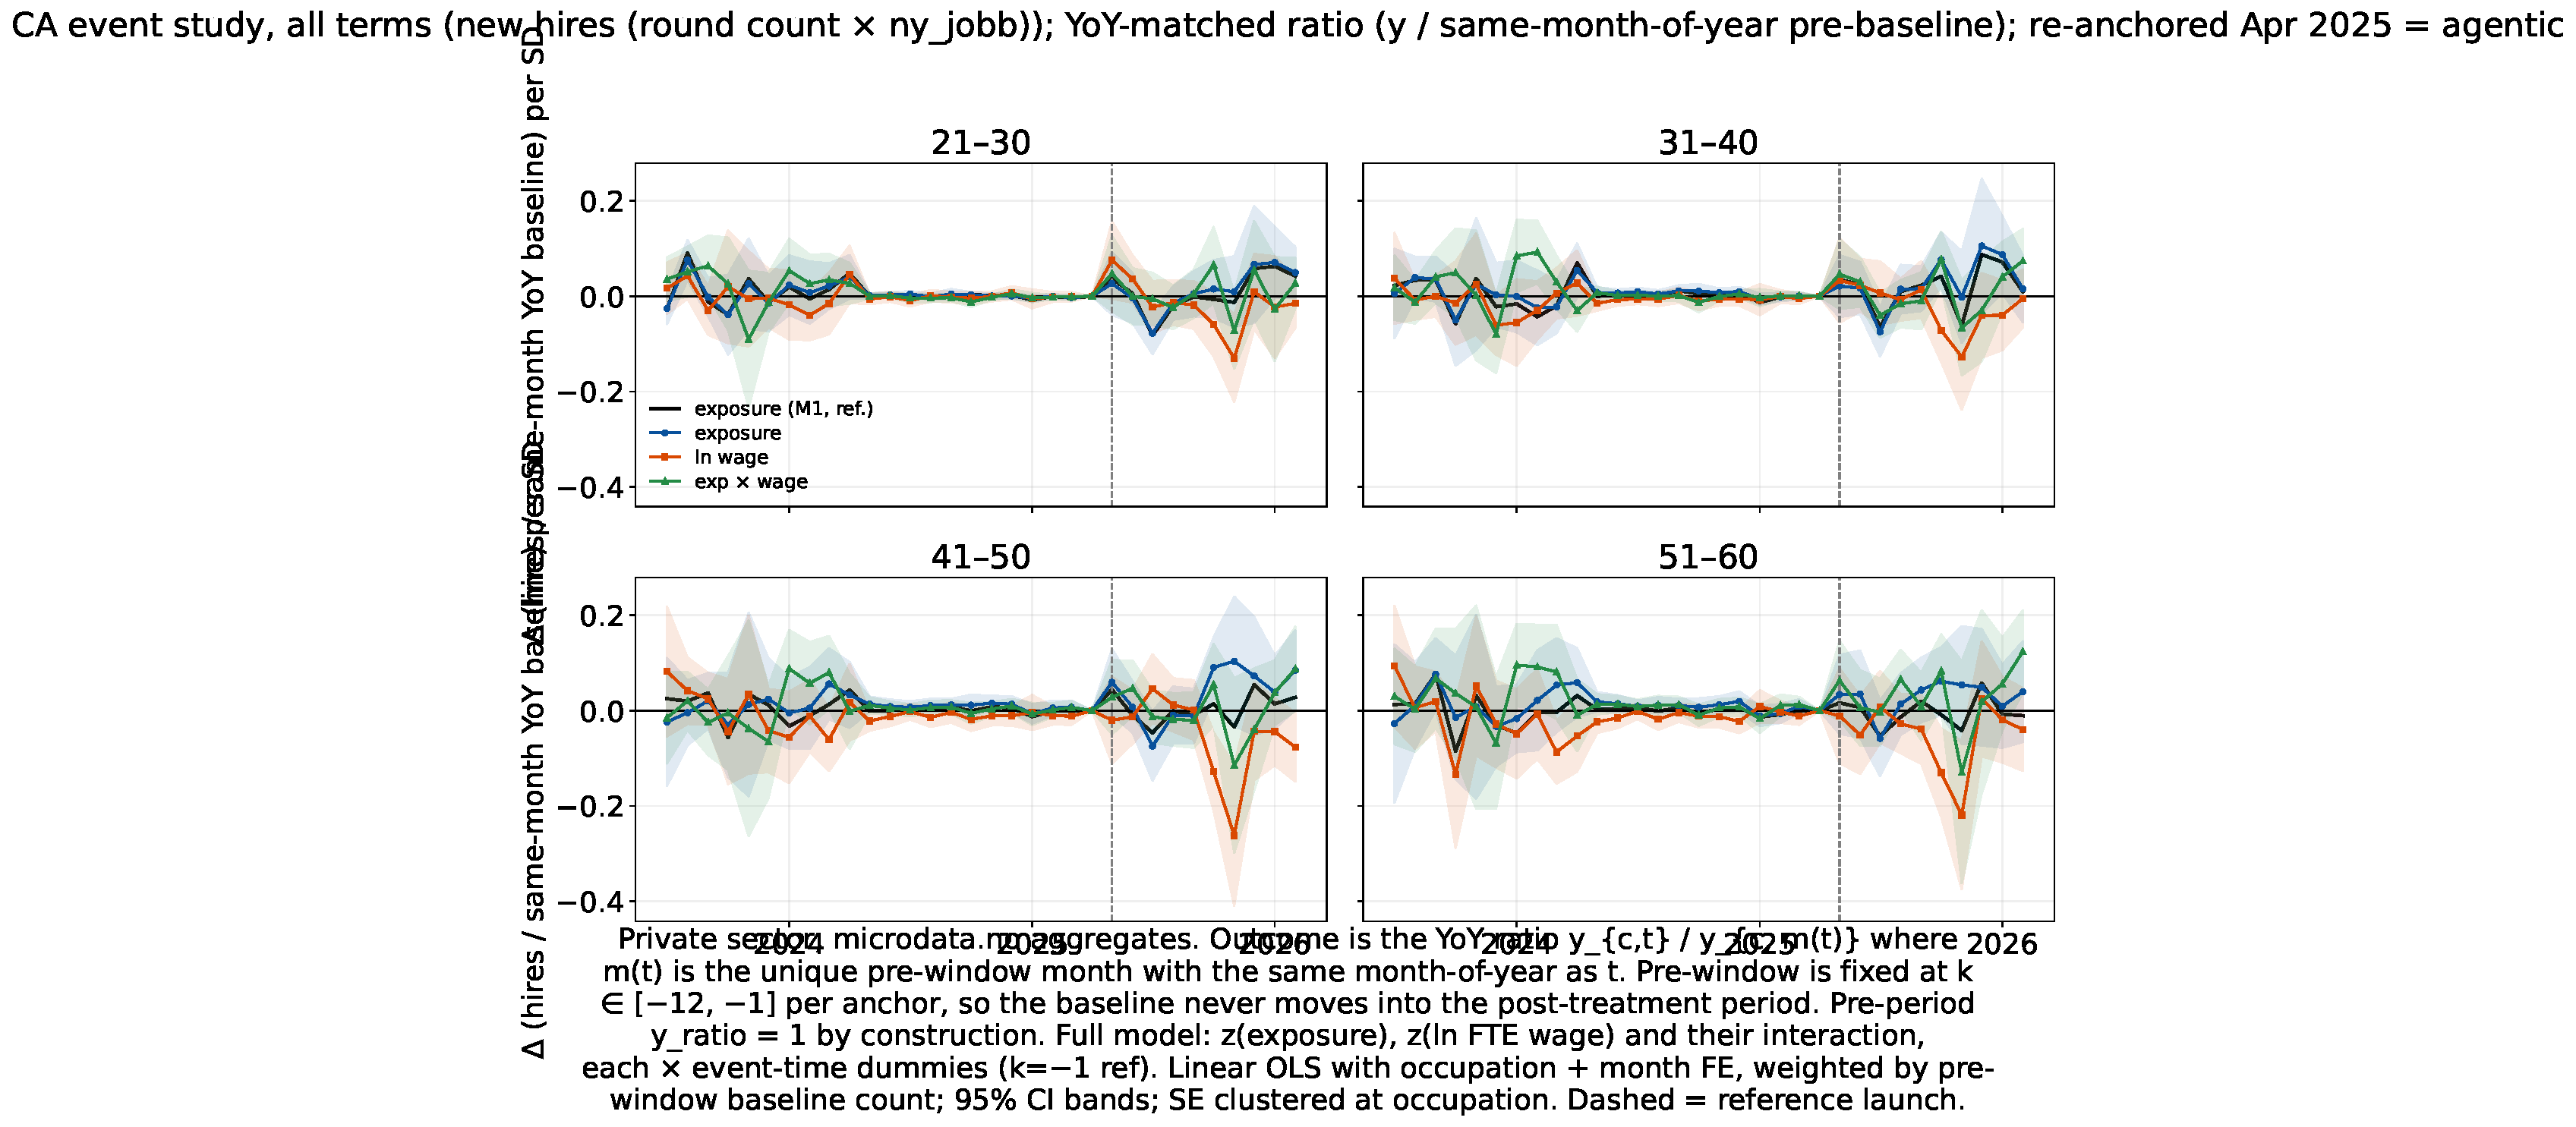
\includegraphics[width=\textwidth,height=0.42\textheight,keepaspectratio]{figure_ca_es_yoy_agentic_nyjobb.pdf}
  \caption{YoY-matched CA event study, new hires --- ChatGPT anchor
           (top), agentic anchor (bottom). Coefficients are
           $\Delta(y_{c,t}/y_{c, m(t)})$ per SD.}
\end{figure}

% =====================================================================
\clearpage
\section{Robustness: YoY-matched pooled DiD (microdata.no, linear OLS)}

\noindent
Pooled-DiD counterpart to Section~9, mirroring Section~8's table format.
Same kk encoding as Sections~2 and~8: each pre-period month is its own
control level, all post months collapse to ``POST'' with the reference
month ($k=-1$) omitted. The POST coefficient is the average post-period
effect on the YoY ratio.

\subsection{Employment (count)}
\begin{table}[H]\centering
\caption{YoY-matched CA pooled DiD on private-sector employment headcount (YoY ratio ($y_{c,t} / y_{c, m(t)}^{\,\mathrm{pre}}$)), by age group}
\label{tab:ca_did_yoy_combined_count}
\small
\begin{tabular}{lcccccc}
\toprule
 & \multicolumn{3}{c}{ChatGPT (ref.\ Oct 2022)} & \multicolumn{3}{c}{Agentic (ref.\ Apr 2025)} \\
\cmidrule(lr){2-4} \cmidrule(lr){5-7}
 & (1) & (2) & (3) & (4) & (5) & (6) \\
\midrule
\multicolumn{7}{@{}l}{\textit{Panel A: ages 21–30}} \\
Exposure $\times$ Post & +0.0199** &  & +0.0105 & -0.0128** &  & -0.0124** \\
 & (0.0079) &  & (0.0081) & (0.0062) &  & (0.0061) \\
ln wage $\times$ Post &  & +0.0429*** & +0.0422*** &  & -0.0041 & -0.0013 \\
 &  & (0.0117) & (0.0131) &  & (0.0059) & (0.0053) \\
Exp $\times$ wage $\times$ Post &  &  & +0.0154 &  &  & -0.0050 \\
 &  &  & (0.0119) &  &  & (0.0068) \\
\quad Observations & \multicolumn{3}{c}{19,288} & \multicolumn{3}{c}{11,954} \\
\quad Occupations & \multicolumn{3}{c}{387} & \multicolumn{3}{c}{385} \\
\midrule
\multicolumn{7}{@{}l}{\textit{Panel B: ages 31–40}} \\
Exposure $\times$ Post & +0.0288*** &  & +0.0183*** & +0.0072* &  & +0.0035 \\
 & (0.0070) &  & (0.0069) & (0.0040) &  & (0.0044) \\
ln wage $\times$ Post &  & +0.0304*** & +0.0204*** &  & +0.0092*** & +0.0073** \\
 &  & (0.0067) & (0.0064) &  & (0.0035) & (0.0037) \\
Exp $\times$ wage $\times$ Post &  &  & +0.0054 &  &  & -0.0001 \\
 &  &  & (0.0073) &  &  & (0.0038) \\
\quad Observations & \multicolumn{3}{c}{19,410} & \multicolumn{3}{c}{11,950} \\
\quad Occupations & \multicolumn{3}{c}{384} & \multicolumn{3}{c}{384} \\
\midrule
\multicolumn{7}{@{}l}{\textit{Panel C: ages 41–50}} \\
Exposure $\times$ Post & -0.0084 &  & -0.0133** & -0.0075** &  & -0.0061* \\
 & (0.0062) &  & (0.0064) & (0.0032) &  & (0.0034) \\
ln wage $\times$ Post &  & +0.0024 & +0.0085 &  & -0.0054* & -0.0024 \\
 &  & (0.0066) & (0.0070) &  & (0.0033) & (0.0034) \\
Exp $\times$ wage $\times$ Post &  &  & +0.0126** &  &  & +0.0036 \\
 &  &  & (0.0063) &  &  & (0.0029) \\
\quad Observations & \multicolumn{3}{c}{19,404} & \multicolumn{3}{c}{11,885} \\
\quad Occupations & \multicolumn{3}{c}{385} & \multicolumn{3}{c}{383} \\
\midrule
\multicolumn{7}{@{}l}{\textit{Panel D: ages 51–60}} \\
Exposure $\times$ Post & -0.0009 &  & -0.0046 & -0.0059** &  & -0.0042 \\
 & (0.0061) &  & (0.0064) & (0.0029) &  & (0.0030) \\
ln wage $\times$ Post &  & +0.0080 & +0.0085 &  & -0.0035 & -0.0027 \\
 &  & (0.0062) & (0.0068) &  & (0.0030) & (0.0031) \\
Exp $\times$ wage $\times$ Post &  &  & +0.0147** &  &  & +0.0112*** \\
 &  &  & (0.0070) &  &  & (0.0034) \\
\quad Observations & \multicolumn{3}{c}{19,289} & \multicolumn{3}{c}{11,875} \\
\quad Occupations & \multicolumn{3}{c}{388} & \multicolumn{3}{c}{384} \\
\midrule
Occupation FE & Yes & Yes & Yes & Yes & Yes & Yes \\
Month FE & Yes & Yes & Yes & Yes & Yes & Yes \\
\bottomrule
\end{tabular}
\begin{minipage}{\linewidth}\vspace{2pt}\footnotesize
\emph{Notes:} Linear OLS (\texttt{fixest::feols}) on the microdata.no cell aggregates (private sector, sektor = 2). Outcome is the YoY ratio $y_{c,t} / y_{c, m(t)}$ where $m(t)$ is the unique pre-window month (within $k \in [-12, -1]$ per anchor) with the same month-of-year as $t$. The pre-window is fixed at $k \in [-12, -1]$, so the baseline never enters the post-treatment region even for $k \geq 12$. Columns (1)--(3): ChatGPT window (Oct 2022 $=k{=}{-}1$, through 2025m4); (4)--(6): agentic (Apr 2025 $=k{=}{-}1$, from 2023m7). Each coefficient is the average post-period effect on the YoY ratio relative to the reference month ($k{=}{-}1$). M1 = exposure only, M2 = ln wage only, M3 = both $+$ interaction. Treatments standardized: $z(\text{exp})$ = Eloundou $\beta$ (pooled), $z(\text{lnw})$ = ln full-time-equivalent wage within age group. Cells weighted by the pre-window baseline count. SE clustered at occupation in parentheses. $^{*}p<0.10$, $^{**}p<0.05$, $^{***}p<0.01$.
\end{minipage}
\end{table}

\clearpage
\subsection{New hires (nyjobb)}
\begin{table}[H]\centering
\caption{YoY-matched CA pooled DiD on private-sector new hires = round(count $\times$ ny\_jobb) (YoY ratio ($y_{c,t} / y_{c, m(t)}^{\,\mathrm{pre}}$)), by age group}
\label{tab:ca_did_yoy_combined_nyjobb}
\small
\begin{tabular}{lcccccc}
\toprule
 & \multicolumn{3}{c}{ChatGPT (ref.\ Oct 2022)} & \multicolumn{3}{c}{Agentic (ref.\ Apr 2025)} \\
\cmidrule(lr){2-4} \cmidrule(lr){5-7}
 & (1) & (2) & (3) & (4) & (5) & (6) \\
\midrule
\multicolumn{7}{@{}l}{\textit{Panel A: ages 21–30}} \\
Exposure $\times$ Post & -0.0238* &  & -0.0314** & +0.0032 &  & +0.0083 \\
 & (0.0126) &  & (0.0125) & (0.0104) &  & (0.0112) \\
ln wage $\times$ Post &  & +0.0121 & +0.0177 &  & -0.0160 & -0.0163 \\
 &  & (0.0142) & (0.0140) &  & (0.0126) & (0.0137) \\
Exp $\times$ wage $\times$ Post &  &  & -0.0311** &  &  & +0.0050 \\
 &  &  & (0.0126) &  &  & (0.0128) \\
\quad Observations & \multicolumn{3}{c}{17,015} & \multicolumn{3}{c}{10,262} \\
\quad Occupations & \multicolumn{3}{c}{359} & \multicolumn{3}{c}{356} \\
\midrule
\multicolumn{7}{@{}l}{\textit{Panel B: ages 31–40}} \\
Exposure $\times$ Post & -0.0170 &  & -0.0397** & +0.0217* &  & +0.0331** \\
 & (0.0168) &  & (0.0161) & (0.0120) &  & (0.0131) \\
ln wage $\times$ Post &  & +0.0203 & +0.0422** &  & -0.0058 & -0.0210 \\
 &  & (0.0174) & (0.0167) &  & (0.0154) & (0.0160) \\
Exp $\times$ wage $\times$ Post &  &  & -0.0658*** &  &  & +0.0169 \\
 &  &  & (0.0182) &  &  & (0.0137) \\
\quad Observations & \multicolumn{3}{c}{16,785} & \multicolumn{3}{c}{10,119} \\
\quad Occupations & \multicolumn{3}{c}{365} & \multicolumn{3}{c}{356} \\
\midrule
\multicolumn{7}{@{}l}{\textit{Panel C: ages 41–50}} \\
Exposure $\times$ Post & -0.0265 &  & -0.0679*** & +0.0072 &  & +0.0397** \\
 & (0.0187) &  & (0.0161) & (0.0122) &  & (0.0154) \\
ln wage $\times$ Post &  & +0.0235 & +0.0604*** &  & -0.0328* & -0.0535*** \\
 &  & (0.0200) & (0.0182) &  & (0.0178) & (0.0200) \\
Exp $\times$ wage $\times$ Post &  &  & -0.0753*** &  &  & +0.0084 \\
 &  &  & (0.0216) &  &  & (0.0148) \\
\quad Observations & \multicolumn{3}{c}{16,000} & \multicolumn{3}{c}{9,707} \\
\quad Occupations & \multicolumn{3}{c}{361} & \multicolumn{3}{c}{359} \\
\midrule
\multicolumn{7}{@{}l}{\textit{Panel D: ages 51–60}} \\
Exposure $\times$ Post & -0.0105 &  & -0.0618*** & -0.0020 &  & +0.0286 \\
 & (0.0207) &  & (0.0177) & (0.0135) &  & (0.0177) \\
ln wage $\times$ Post &  & +0.0396 & +0.0714*** &  & -0.0334* & -0.0461** \\
 &  & (0.0243) & (0.0230) &  & (0.0193) & (0.0225) \\
Exp $\times$ wage $\times$ Post &  &  & -0.0895*** &  &  & +0.0349 \\
 &  &  & (0.0263) &  &  & (0.0235) \\
\quad Observations & \multicolumn{3}{c}{14,746} & \multicolumn{3}{c}{8,938} \\
\quad Occupations & \multicolumn{3}{c}{357} & \multicolumn{3}{c}{347} \\
\midrule
Occupation FE & Yes & Yes & Yes & Yes & Yes & Yes \\
Month FE & Yes & Yes & Yes & Yes & Yes & Yes \\
\bottomrule
\end{tabular}
\begin{minipage}{\linewidth}\vspace{2pt}\footnotesize
\emph{Notes:} Linear OLS (\texttt{fixest::feols}) on the microdata.no cell aggregates (private sector, sektor = 2). Outcome is the YoY ratio $y_{c,t} / y_{c, m(t)}$ where $m(t)$ is the unique pre-window month (within $k \in [-12, -1]$ per anchor) with the same month-of-year as $t$. The pre-window is fixed at $k \in [-12, -1]$, so the baseline never enters the post-treatment region even for $k \geq 12$. Columns (1)--(3): ChatGPT window (Oct 2022 $=k{=}{-}1$, through 2025m4); (4)--(6): agentic (Apr 2025 $=k{=}{-}1$, from 2023m7). Each coefficient is the average post-period effect on the YoY ratio relative to the reference month ($k{=}{-}1$). M1 = exposure only, M2 = ln wage only, M3 = both $+$ interaction. Treatments standardized: $z(\text{exp})$ = Eloundou $\beta$ (pooled), $z(\text{lnw})$ = ln full-time-equivalent wage within age group. Cells weighted by the pre-window baseline count. SE clustered at occupation in parentheses. $^{*}p<0.10$, $^{**}p<0.05$, $^{***}p<0.01$.
\end{minipage}
\end{table}

% =====================================================================
\clearpage
\section*{References}

\begin{description}
  \item[LORV (2026)] Lindenlaub, I., R. Oh, M.~A. Rodríguez \& L. Veldkamp.
  ``Beyond Exposure: Predicting AI Adoption Based on Comparative
  Advantage.'' Working paper, May 22, 2026. Documents the gap between AI
  exposure and observed adoption in German DiWaBe-IEB linked data, derives
  the task-level adoption condition in equation~\eqref{eq:lorv}, and shows
  that a comparative-advantage index accounts for 60\% of cross-occupation
  adoption variation versus 14\% for exposure alone.
  \item[Yagan (2020)] Yagan, D. ``Employment Hysteresis from the Great
  Recession.'' \emph{Journal of Political Economy}, 128(7), 2505--2558.
  The relative-outcome specification (eq.~(2): $e_{it} \equiv
  \mathrm{EMPLOYED}_{it} - \tfrac{1}{8}\sum_{s=1999}^{2006}
  \mathrm{EMPLOYED}_{is}$, see also Fig.~4C for earnings and Fig.~6B for
  the ratio variant) used in Sections~7--8 above as the cell-level
  Yagan-diff and Yagan-ratio outcomes.
\end{description}

\end{document}
